% Gelfand seminar notes, 1980-81: source pages P000916-P000980.
% Russian diplomatic transcription (AI-made, checked against the scans), cut page by page from the cumulative working reader A4-reader-chapters01-34-complete-first1527-separated-diplomatic-r50.
% \SourcePage{GELFAND-Pnnnnnn}{label} starts a scanned page; the second argument is the number written
% on the page, if any. Editorial notes give the page, a label and the transcriber's remark; \Unclear
% marks a doubtful reading.
\SourcePage{GELFAND-P000916}{unlabelled}

\begin{equation*}
 (1)\quad\left\{
 \begin{aligned}
 \frac{\partial w}{\partial z}+\operatorname{div}\vec u&=0\\
 \vec u_t+(u\nabla)u+w\frac{\partial\vec u}{\partial z}+\nabla h&=0
 \end{aligned}\right.
\end{equation*}

\begin{equation*}
 \frac{\partial p}{\partial z}+1=0
 \quad\Longrightarrow\quad p=-z+h(\vec r,t)
\end{equation*}
\Unclear{GELFAND-P000916}{pressure-coordinate}{Координата в аргументе $h$ читается как $\vec r$.}
\end{GelfandAdjacentEvidence}
\begin{GelfandAdjacentEvidence}{GELFAND-P000916}{2}


\begin{equation*}
 (1)_3\quad\left\{h_t+\operatorname{div}\int_0^h\vec u\,dz=0\right.
\end{equation*}
\Unclear{GELFAND-P000916}{equation-zeros}{Четыре знака после равенства читаются как 0. У нескольких разомкнут правый контур.}
\end{GelfandAdjacentEvidence}
\begin{GelfandAdjacentEvidence}{GELFAND-P000916}{3}


$(1)$ --- система ур-й Бенни

Манин [подписано снизу: и др.] --- 1-мерный случай.
\SourceFigure{GELFAND-P000916}{manin-insertion}{Приписка «и др.» под фамилией Манина.}
\end{GelfandAdjacentEvidence}
\begin{GelfandAdjacentEvidence}{GELFAND-P000916}{4}


\uwave{Захаров} а) в 1-мерном случае вывел счёт. з.с-ний, их намного больше
\Unclear{GELFAND-P000916}{zakharov-first-verb}{Глагол читается как «вывел».}
\end{GelfandAdjacentEvidence}
\begin{GelfandAdjacentEvidence}{GELFAND-P000916}{5}

\Unclear{GELFAND-P000916}{zakharov-second-verb}{После «счёт.» читается сокращение «з.с-ний».}
\end{GelfandAdjacentEvidence}
\begin{GelfandAdjacentEvidence}{GELFAND-P000916}{6}

\SourceFigure{GELFAND-P000916}{zakharov-first-line}{Конец пункта а). Последние слова читаются как «их намного больше».}
\end{GelfandAdjacentEvidence}
\begin{GelfandAdjacentEvidence}{GELFAND-P000916}{7}


б) другая гам. структура (более простая)

в) что-то для 2-мерной зав. (с гамильтоновостью)

Идея: переинтерпрет. задачи.
\Unclear{GELFAND-P000916}{idea-word}{Сокращение перед «задачи» читается как «переинтерпрет.».}
\end{GelfandAdjacentEvidence}
\begin{GelfandAdjacentEvidence}{GELFAND-P000916}{8}


\uline{И.М.Г.}\quad \uwave{Коллективные дифф. ур-я:}

когда частицы не взаимод. неп., но
[зачёркнуто: неразборчиво]
[вписано сверху: заряжены и] вместе созд. поле, к-рое
[между строками: (электрическ. поле)]
действ. на каждую в отдельности.

\Incomplete{GELFAND-P000916}{cancelled-word}{Короткая запись после «но» зачёркнута. Чтение не установлено.}
\end{GelfandAdjacentEvidence}
\begin{GelfandAdjacentEvidence}{GELFAND-P000916}{9}

\Unclear{GELFAND-P000916}{interaction-abbreviation}{Сокращение после «взаимод.» читается предположительно как «неп.».}
\end{GelfandAdjacentEvidence}
\begin{GelfandAdjacentEvidence}{GELFAND-P000916}{10}

\SourceFigure{GELFAND-P000916}{inserted-words}{Вставка «заряжены и» с длинной выноской.}
\end{GelfandAdjacentEvidence}
\begin{GelfandAdjacentEvidence}{GELFAND-P000916}{11}

\Unclear{GELFAND-P000916}{parenthetic-field}{Первое слово в скобках читается предположительно как «электрическ.».}
\end{GelfandAdjacentEvidence}
\begin{GelfandAdjacentEvidence}{GELFAND-P000916}{12}


След. раздел за обыкн. дифф. ур-ями.
\Unclear{GELFAND-P000916}{last-clause}{В конце строки чтение «След. раздел за обыкн.» предположительное. Над последним сокращением виден отдельный штрих.}
\end{GelfandAdjacentEvidence}



\Needspace{7\baselineskip}
\begin{GelfandAdjacentEvidence}{GELFAND-P000917}{1}
\SourcePage{GELFAND-P000917}{unlabelled}

\uuline{22.9.80 г.}\qquad \uuline{Сем. Гельфанда.}

\uline{Фукс.} Есть мн-ие с особ. (алгебр., компл.) и есть стратификация.
\begin{equation*}
 (1)\quad X=X_{2n}\supset X_{2n-2}\supset X_{n-3}\supset X_{n-4}\supset\ldots
\end{equation*}
\Unclear{GELFAND-P000917}{filtration-indices}{В двух последних явно записанных индексах перед $n$ нет цифры 2.}
\end{GelfandAdjacentEvidence}
\begin{GelfandAdjacentEvidence}{GELFAND-P000917}{2}


$X_i\setminus X_{i-1}$ --- $i$-мерное мн-ие.

Около данного страта всё устроено одинаково (вся окрестность).

Рассм. сингул. симплексы пр-ва $X$, облад. нек-рыми доп. св-вами.

\begin{equation*}
 \sigma_j\qquad \dim\sigma_j=j
\end{equation*}
\Unclear{GELFAND-P000917}{dimension-cancellation}{Между $\dim$ и $\sigma_j$ зачёркнут неразборчивый знак.}
\end{GelfandAdjacentEvidence}
\begin{GelfandAdjacentEvidence}{GELFAND-P000917}{3}


\begin{equation*}
 (2)\quad \dim(\sigma_j\cap X_{2n-i})=j-2i
\end{equation*}
\Unclear{GELFAND-P000917}{dimension-condition}{В (2) слева читается индекс $2n-i$, справа --- $j-2i$.}
\end{GelfandAdjacentEvidence}
\begin{GelfandAdjacentEvidence}{GELFAND-P000917}{4}


В этих когом. есть двойств. Пуанкаре. Это другие когомологии.

\uline{Пример:} Две 2-мерн. сферы, склеенные в 1-й точке
\Unclear{GELFAND-P000917}{example-gluing}{Цифра читается как 1. Конец слова «точке» обведён.}
\end{GelfandAdjacentEvidence}
\begin{GelfandAdjacentEvidence}{GELFAND-P000917}{5}

\SourceFigure{GELFAND-P000917}{two-spheres-contact}{Два контура со сближением в середине. В узкой области соприкосновения линии обведены повторно.%
\par\smallskip
\begingroup\color{black}\GelfandFitDiagram{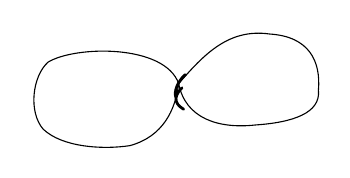
\begin{tikzpicture}[x=1.05cm,y=1.05cm,line cap=round]
\draw (-.02,.12).. controls (-.19,.60) and (-1.27,.58) .. (-1.60,.38)
.. controls (-1.79,.21) and (-1.84,-.22) .. (-1.66,-.43)
.. controls (-1.43,-.65) and (-.94,-.68) .. (-.61,-.63)
.. controls (-.21,-.52) and (-.06,-.20) .. (-.02,.12);
\draw (-.02,.12).. controls (.29,.48) and (.59,.79) .. (1.08,.72)
.. controls (1.56,.69) and (1.70,.39) .. (1.67,.04)
.. controls (1.70,-.24) and (1.35,-.35) .. (.91,-.38)
.. controls (.46,-.43) and (.06,-.30) .. (-.02,.12);
\draw[line width=1pt] (-.05,-.06).. controls (-.09,.03) and (-.02,.16) .. (.06,.23)
(.04,-.19).. controls (-.10,-.11) and (-.06,-.01) .. (.02,.07);
\end{tikzpicture}}\endgroup}
\end{GelfandAdjacentEvidence}
\begin{GelfandAdjacentEvidence}{GELFAND-P000917}{6}


Эти когомологии \uwave{не гомотопически инвариантны}.

\uline{Обычные гомологии:}
\begin{equation*}
 \left\{\begin{array}{ll}
 0 & \mathbb{Z}\\
 1 & 0\\
 2 & \mathbb{Z}\dotplus\mathbb{Z}
 \end{array}\right.
\end{equation*}
\Unclear{GELFAND-P000917}{ordinary-homology-cancellation}{Справа от первой строки зачёркнута короткая запись. Начало похоже на $\mathbb Z$, но запись целиком не читается.}
\end{GelfandAdjacentEvidence}
\begin{GelfandAdjacentEvidence}{GELFAND-P000917}{7}


Они не удовл. двойств. Пуанкаре (видно сразу).

\uline{Гом. Макферсона}
\begin{equation*}
 \left\{\begin{array}{ll}
 0 & \mathbb{Z}\dotplus\mathbb{Z}\\
 1 & 0\\
 2 & \mathbb{Z}\dotplus\mathbb{Z}.
 \end{array}\right.
\end{equation*}
\SourceFigure{GELFAND-P000917}{homology-sum-signs}{Во всех трёх записях суммы над плюсом поставлена точка.}
\end{GelfandAdjacentEvidence}
\begin{GelfandAdjacentEvidence}{GELFAND-P000917}{8}


\SourceFigure{GELFAND-P000917}{forbidden-simplex}{Ломаная соединяет две отмеченные точки и проходит через место соприкосновения контуров.%
\par\smallskip
\begingroup\color{black}\GelfandFitDiagram{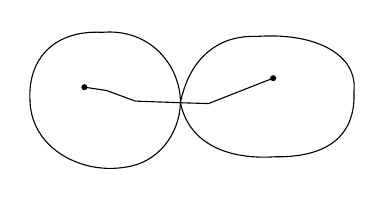
\begin{tikzpicture}[x=1.08cm,y=1.04cm,line cap=round]
\draw (1.80,0) .. controls (1.80,.45) and (1.45,.91) .. (.88,.86)
 .. controls (.31,.89) and (.01,.53) .. (.03,.05)
 .. controls (.03,-.54) and (.61,-.87) .. (1.13,-.79)
 .. controls (1.55,-.74) and (1.79,-.37) .. (1.80,0);
\draw (1.80,0) .. controls (1.89,.47) and (2.18,.83) .. (2.70,.81)
 .. controls (3.39,.86) and (3.89,.59) .. (3.84,.13)
 .. controls (3.86,-.36) and (3.58,-.67) .. (2.91,-.66)
 .. controls (2.30,-.70) and (1.89,-.46) .. (1.80,0);
\draw (.67,.19)--(.93,.15)--(1.27,.02)--(1.80,0)--(2.13,-.01)--(2.89,.30);
\fill (.67,.19) circle (1.1pt) (2.89,.30) circle (1.1pt);
\end{tikzpicture}}\endgroup}
\end{GelfandAdjacentEvidence}
\begin{GelfandAdjacentEvidence}{GELFAND-P000917}{9}

Такой симплекс \uwave{запрещается}.

\uline{Гипотеза:} совпадают с $L_2$-когомологиями.

(этим \uline{интересовался Борель})

Пусть есть ровно одна изолир. особенность. Тогда MF-когом.
\SourceFigure{GELFAND-P000917}{macpherson-gloss}{Под «MF-когом.» подписано «(Макферс.)».}
\end{GelfandAdjacentEvidence}
\begin{GelfandAdjacentEvidence}{GELFAND-P000917}{10}


\begin{equation*}
 \left.\begin{aligned}
 \text{в разм.}\ >\frac{\dim X}{2}\quad &\text{совп. с обычными,}\\
 \text{в разм.}\ <\frac{\dim X}{2}\quad &\text{из двойств. Пуанкаре.}
 \end{aligned}\right]\quad\text{это опр. Делиня}
\end{equation*}
\SourceFigure{GELFAND-P000917}{deligne-bracket}{Справа от скобки стоит приписка «это опр. Делиня».}
\end{GelfandAdjacentEvidence}



\Needspace{7\baselineskip}
\begin{GelfandAdjacentEvidence}{GELFAND-P000918}{1}
\SourcePage{GELFAND-P000918}{unlabelled}

Опр. Делиня в более общей ситуации (индуктивное)

\uline{М.И. Граев.}

Из работ Гельф.-Гинд.-Шап.
\begin{equation*}
\begin{array}{ll}
 \text{ФА} & 13:2\\
 \text{ФА} & 14:4
\end{array}
\end{equation*}
\Unclear{GELFAND-P000918}{reference-author-abbreviation}{Последняя фамилия сокращена как «Шап.». Справа указаны «ФА 13:2» и «ФА 14:4».}
\end{GelfandAdjacentEvidence}
\begin{GelfandAdjacentEvidence}{GELFAND-P000918}{2}


$\mathcal D\subset\mathbb R^n$,

$(n+k-1)$-пар. сем-во кривых
\Unclear{GELFAND-P000918}{family-parameter-cancellation}{$(n+k-1)$ вписано сверху и соединено с местом зачёркнутой записи. Предыдущий знак неразборчив.}
\end{GelfandAdjacentEvidence}
\begin{GelfandAdjacentEvidence}{GELFAND-P000918}{3}


\begin{equation*}
 x_i=\varphi_i(x_1,\xi),\qquad
 \xi=(\xi_1,\ldots,\xi_n),\qquad \xi\in\Gamma
\end{equation*}

Интегр. преобр.
\begin{equation*}
 \xi=(\xi_1,\ldots,\xi_{n+k-1}),
\end{equation*}
\Unclear{GELFAND-P000918}{parameter-vector-length}{Первый перечень заканчивается $\xi_n$, второй --- $\xi_{n+k-1}$.}
\end{GelfandAdjacentEvidence}
\begin{GelfandAdjacentEvidence}{GELFAND-P000918}{4}

$f(x),\qquad \operatorname{supp}f\subset\mathcal D$
\begin{equation*}
 F(\xi)=I_\chi f
 =\int f(x_1,\varphi_1(x_1,\xi),\ldots,\varphi_n(x_1,\xi))
         \chi(x_1,\xi)\,dx_1
\end{equation*}
\Unclear{GELFAND-P000918}{integral-first-index}{Первый индекс у $\varphi$ под интегралом читается как 1.}
\end{GelfandAdjacentEvidence}
\begin{GelfandAdjacentEvidence}{GELFAND-P000918}{5}

\SourceFigure{GELFAND-P000918}{positive-weight-callout}{Стрелка от приписки к множителю $\chi$.%
\par\smallskip
\begingroup\color{black}\GelfandFitDiagram{\begin{tikzpicture}
\node[anchor=west,align=left,inner sep=1pt] (W) at (1.22,.88) {фикс всюд.\\ф-я \({}>0\).};
\node at (0,0) {$\chi$};
\draw[->] (.97,.65)--(.23,.15);
\end{tikzpicture}}\endgroup}
\end{GelfandAdjacentEvidence}
\begin{GelfandAdjacentEvidence}{GELFAND-P000918}{6}


Интересно найти такие мн-зия кривых, для к-рых

\(\exists\) лок. формула обращ. (восст. по инт. по кривым, прох. через эту точку или беск. близкую)

Такие мн-зия кривых наз. \uwave{допустимыми}.

$\forall x^0\in\mathcal D$ опр. оператор \(F(\xi)\longrightarrow\mathcal H_{x^0}F\).
\Unclear{GELFAND-P000918}{differential-operator-glyph}{Фигурная буква оператора передана как $\mathcal H$.}
\end{GelfandAdjacentEvidence}
\begin{GelfandAdjacentEvidence}{GELFAND-P000918}{7}


\begin{equation*}
 \Gamma_{x^0}\qquad x_i^0=\varphi_i(x_i^0,\xi)
 \qquad\dim\Gamma_{x^0}=k
\end{equation*}
\Unclear{GELFAND-P000918}{fixed-point-coordinate-index}{В первом аргументе $\varphi_i$ отчётливо видна точка над нижним индексом $i$.}
\end{GelfandAdjacentEvidence}
\begin{GelfandAdjacentEvidence}{GELFAND-P000918}{8}

\Unclear{GELFAND-P000918}{gamma-subscript-cancellation}{Под $x$ в индексе левой $\Gamma$ зачёркнут неразборчивый знак.}
\end{GelfandAdjacentEvidence}
\begin{GelfandAdjacentEvidence}{GELFAND-P000918}{9}


\(\mathcal H_{x^0}\) --- дифф. форма на
\Incomplete{GELFAND-P000918}{trailing-form-on}{Строка оканчивается словом «на». Дополнение не записано.}
\end{GelfandAdjacentEvidence}
\begin{GelfandAdjacentEvidence}{GELFAND-P000918}{10}


\begin{equation*}
 \mathcal H_{x^0}F=
 \sum a_{ij}(x_1^0,\xi)\frac{\partial F}{\partial\xi_j}\,d\xi_i
 + F\sum b_i(x_1^0,\xi)\,d\xi_i
\end{equation*}

Оператор $\mathcal H_{x^0}$ наз. \uline{допустимыми}, если $\forall$ ф-и $f$ дифф. форма

\(\mathcal H_{x^0}I_\chi f\) явл. замкнутой.

\(k>1\ \Rightarrow\) это полное опред.

Если $k=1$, то автоматич. замкнута и треб., чтобы ф-л
\begin{equation*}
 f\mapsto\int\mathcal H_{x_0}I_\chi f
\end{equation*}
был сосредоточен в т. \(x_0\).
\Unclear{GELFAND-P000918}{base-point-zero-position}{В интеграле и в следующей строке 0 стоит снизу. В предыдущих формулах 0 у $x$ стоит сверху.}
\end{GelfandAdjacentEvidence}
\begin{GelfandAdjacentEvidence}{GELFAND-P000918}{11}


Тривиальный ф-л: \(\underline{\mathcal H_{x^0}F=d(\mu F)}\)
\SourceFigure{GELFAND-P000918}{trivial-functional-underline}{Формула тривиального функционала подчёркнута.}
\end{GelfandAdjacentEvidence}


Важен фактор по трив. ф-лам.


\clearpage
\pdfbookmark[0]{Глава 18}{gelfand-archive-chapter-18}
\section*{Глава 18}
\Needspace{7\baselineskip}
\begin{GelfandAdjacentEvidence}{GELFAND-P000919}{1}
\SourcePage{GELFAND-P000919}{unlabelled}

\uuline{13.10.80 г.}\qquad \uline{Сем. Гельфанда.}

\uline{И.М. Гельфанд.} Рассм. уравнение
\begin{equation*}
 f(z_1,\ldots,z_n;w_1,\ldots,w_n)=0
 \tag{1}
\end{equation*}

Пример: рассм. д.у. 2-го порядка
\begin{equation*}
 y''=f(x,y,y')
 \tag{2}
\end{equation*}
\Unclear{GELFAND-P000919}{formula-02-cancelled-superscript}{Над вторым аргументом $y$ зачёркнут надстрочный знак. Его чтение не установлено.}
\end{GelfandAdjacentEvidence}
\begin{GelfandAdjacentEvidence}{GELFAND-P000919}{2}


Тогда
\begin{equation*}
 y=\varphi(x,\xi,\eta)
 \tag{3}
\end{equation*}
\Unclear{GELFAND-P000919}{formula-03-overwritten-function}{Густо обведённая буква читается как $\varphi$.}
\end{GelfandAdjacentEvidence}
\begin{GelfandAdjacentEvidence}{GELFAND-P000919}{3}


Обратно, если есть сем-во (3), то по нему строится д.у. 2-го пор.

более обще:
\begin{equation*}
 F(x,y,\xi,\eta)=0
 \tag{4}
\end{equation*}
\Unclear{GELFAND-P000919}{formula-04-separator}{В (4) после $y$ стоит запятая.}
\end{GelfandAdjacentEvidence}
\begin{GelfandAdjacentEvidence}{GELFAND-P000919}{4}


Можно рассм. $\xi,\eta$ как точку и строить двойств. дифф. ур-е.

(1) задаёт $n$-парам. сем-во гиперповерхностей.

(5) \uwave{Задача:} найти геометрию, связ. с этим сем-вом.

Можно делать замены переменных. Напр., в ур-и прямых
\begin{equation*}
 \xi x+\eta y=1
 \tag{6}
\end{equation*}

(7) \uwave{Задача:} как можно узнать, свод. ли сем-во (4) к сем-ву прямых (6).

\uline{Замены:}
\begin{equation*}
 \left\{\begin{aligned}
 x_1&=u(x,y)\\
 y_1&=v(x,y
 \end{aligned}\right.
 \qquad
 \left\{\begin{aligned}
 \xi_1&=\varphi(\xi,\eta)\\
 \eta_1&=\psi(\xi,\eta)
 \end{aligned}\right.
\end{equation*}
\Unclear{GELFAND-P000919}{substitution-missing-parenthesis}{После $y$ во второй строке левой системы закрывающей скобки нет.}
\end{GelfandAdjacentEvidence}
\begin{GelfandAdjacentEvidence}{GELFAND-P000919}{5}


(8) \uwave{Общее определение:} \uline{двойное расслоение}

(9) элемент --- \uwave{точка и прох. через него кривая}

(кривые из 2-пар. сем-ва)

\SourceFigure{GELFAND-P000919}{double-fibration}{Две проекции с метками $\pi_1$ и $\pi_2$.%
\par\smallskip
\begingroup\color{black}\GelfandFitDiagram{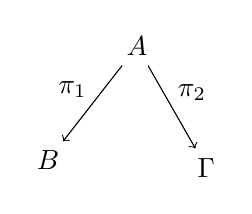
\begin{tikzpicture}
\node (A) at (0,0) {$A$};
\node (B) at (-1.13,-1.45) {$B$};
\node (G) at (.88,-1.54) {$\Gamma$};
\draw[->] (A)--node[above left,inner sep=2pt] {$\pi_1$}(B);
\draw[->] (A)--node[above right,inner sep=2pt] {$\pi_2$}(G);
\end{tikzpicture}}\endgroup
\par
(есть 2 проекции)}
\end{GelfandAdjacentEvidence}


(см. ст. \uwave{Гельфанд}, \uwave{Гиндикин}, \uwave{Шапиро} в ФА)


\Needspace{7\baselineskip}
\begin{GelfandAdjacentEvidence}{GELFAND-P000920}{1}
\SourcePage{GELFAND-P000920}{unlabelled}

(10) \uwave{Требование:} если
\begin{equation*}
 \left\{\begin{aligned}
 \pi_1x&=\pi_1x'\\
 \text{и}\quad\pi_2x&=\pi_2x'
 \end{aligned}\right.
 ,\quad\text{то }x=x'
\end{equation*}

более сильное требование:
\begin{equation*}
 (11)\qquad A\subset B\times\Gamma\quad\text{как \uwave{подмногообразие}}
\end{equation*}
\begin{equation*}
 x\mapsto(\pi_1x,\pi_2x)
\end{equation*}

\uline{Задача:} классифицировать с точн. до диффеоморфизма
\begin{equation*}
 f(z,w)=0,
 \tag{12}
\end{equation*}
с точн. до замен
\begin{equation*}
 \varphi(z)=z_1,\qquad\psi(w)=w_1
\end{equation*}
(всё аналитическое).

(13) Ещё пример: $A=G$ --- группа, $K,H$ --- 2 подгруппы,
\begin{equation*}
 B=H\backslash G,\qquad\Gamma=K\backslash G.
\end{equation*}

(14) \uline{Важный пример:}

$G$ --- группа $GL(n,\mathbb C)$,

$K$ --- подгр. унит. матриц

$H$ --- —\raisebox{-.15ex}{\(\scriptstyle\prime\prime\)}— треуг. матриц

(15) Полезный частн. случай: $n=2$.

Тогда возник. пл. Лобач., орисферы.
\Unclear{GELFAND-P000920}{lobachevsky-abbreviation}{Перед «Лобач.» сокращение читается как «пл.».}
\end{GelfandAdjacentEvidence}
\begin{GelfandAdjacentEvidence}{GELFAND-P000920}{2}


(быть может в $H$ брать 1 на гл. диагонали)
\Unclear{GELFAND-P000920}{subgroup-parenthesis-word}{Начало скобок читается «быть может».}
\end{GelfandAdjacentEvidence}
\begin{GelfandAdjacentEvidence}{GELFAND-P000920}{3}


Раб. из Inventiones о \uwave{сем-вах Сегре.}
\begin{equation*}
 \tau(z,\zeta)=0
 \tag{16}
\end{equation*}

\Unclear{GELFAND-P000920}{right-margin-strokes}{Отдельные неразборчивые штрихи на правом поле на высоте (16).}
\end{GelfandAdjacentEvidence}
\begin{GelfandAdjacentEvidence}{GELFAND-P000920}{4}


\begin{align*}
 z&=(z_1,\quad,z_n;w)\\
 \zeta&=(\zeta_1,\quad,\zeta_{n+1})
\end{align*}
\Unclear{GELFAND-P000920}{formula-16-tuple-gaps}{Между запятыми в обоих наборах оставлены промежутки без видимого многоточия.}
\end{GelfandAdjacentEvidence}
\begin{GelfandAdjacentEvidence}{GELFAND-P000920}{5}


\begin{align*}
 \theta&=d_z\tau=\tau_\alpha\,dz^\alpha+\tau_w\,dw\\
 \theta^\alpha&=dz^\alpha\\
 \theta_\alpha&=d\zeta_\alpha
\end{align*}

При отобр.
\begin{equation*}
 (z,\zeta)\to(f(z),\bar f(\zeta))
 \tag{17}
\end{equation*}
формы преобр. так:

\begin{equation*}
 \begin{aligned}
 \theta^*&=\theta,\\
 \theta^{\alpha*}&=\left(\frac{\partial f^\alpha}{\partial z^\beta}
       -\frac{\tau_\beta}{\tau_w}\frac{\partial f^\alpha}{\partial w}\right)\theta^\beta
       +\frac{1}{\tau_w}\frac{\partial f^\alpha}{\partial w}\theta,
 \end{aligned}
 \tag{18}
\end{equation*}
\Incomplete{GELFAND-P000920}{formula-18-upper-cancellation}{После минуса и перед дробью с $\tau_\beta$ зачёркнуто неразборчивое выражение.}
\end{GelfandAdjacentEvidence}
\begin{GelfandAdjacentEvidence}{GELFAND-P000920}{6}

\Unclear{GELFAND-P000920}{formula-18-upper-last-denominator}{В последнем слагаемом знак перед нижним $w$ похож на $\tau$ с угловатой верхней частью. Чтение $\tau_w$ предположительное.}
\end{GelfandAdjacentEvidence}
\begin{GelfandAdjacentEvidence}{GELFAND-P000920}{7}


\begin{equation*}
 \begin{aligned}
 \theta_\alpha^*&=\left(\frac{\partial\bar f}{\partial\zeta_\beta}
     -\frac{\tau^\beta}{\tau^\eta}\frac{\partial f^\alpha}{\partial\eta}
     \right)\theta_\beta+\frac{1}{\tau^\beta}\frac{\partial\bar f_\alpha}{\partial\eta}.
 \end{aligned}
\end{equation*}
\Unclear{GELFAND-P000920}{formula-18-first-numerator}{В первом числителе нижней строки над $f$ стоит черта. Индекса у $f$ не видно.}
\end{GelfandAdjacentEvidence}
\begin{GelfandAdjacentEvidence}{GELFAND-P000920}{8}

\Unclear{GELFAND-P000920}{formula-18-overwritten-denominator}{У знаменателя после минуса верхний индекс предположительно $\eta$. Нижний знак густо зачёркнут или переписан.}
\end{GelfandAdjacentEvidence}
\begin{GelfandAdjacentEvidence}{GELFAND-P000920}{9}

\Unclear{GELFAND-P000920}{formula-18-lower-cancellation}{Между дробью с $\tau^\beta$ и следующей производной длинное петлеобразное зачёркивание.}
\end{GelfandAdjacentEvidence}
\begin{GelfandAdjacentEvidence}{GELFAND-P000920}{10}

\Unclear{GELFAND-P000920}{formula-18-middle-numerator}{У среднего числителя нижней строки виден верхний индекс $\alpha$. Черты над $f$ не видно.}
\end{GelfandAdjacentEvidence}
\begin{GelfandAdjacentEvidence}{GELFAND-P000920}{11}

\Unclear{GELFAND-P000920}{formula-18-final-term}{Последний знаменатель читается $\tau^\beta$, а $\alpha$ у последнего $\bar f$ стоит снизу. После производной множителя не видно.}
\end{GelfandAdjacentEvidence}
\begin{GelfandAdjacentEvidence}{GELFAND-P000920}{12}


[Зачёркнуто: Отсюда.] Пусть
\SourceFigure{GELFAND-P000920}{cancelled-from-here}{Зачёркнутое слово читается как «Отсюда».}
\end{GelfandAdjacentEvidence}


\begin{equation*}
 \tau\mapsto s(z,\zeta)\tau(z,\zeta)
 \tag{19}
\end{equation*}
Тогда


\Needspace{7\baselineskip}
\begin{GelfandAdjacentEvidence}{GELFAND-P000921}{1}
\SourcePage{GELFAND-P000921}{3}

\begin{equation*}
 \left\{\begin{aligned}
 \theta^*&=s\theta\\
 \theta^{\alpha*}&=\theta^\alpha\\
 \theta_\alpha^*&=\theta_\alpha
 \end{aligned}\right.
 \tag{20}
\end{equation*}

и

\begin{equation*}
 \left\{\begin{aligned}
 \theta^*&=u\theta^*\\
 \theta^\alpha&=u^\alpha\theta^\alpha+u^\alpha_\beta\theta^{\beta*}\\
 \theta_\alpha&=v_\alpha\theta^*+v^\beta_\alpha\theta_\beta^*
 \end{aligned}\right.
 \tag{21}
\end{equation*}
\Unclear{GELFAND-P000921}{formula-21-first-left}{Слева в первой строке над $\theta$ густо обведён знак, предположительно звёздочка.}
\end{GelfandAdjacentEvidence}
\begin{GelfandAdjacentEvidence}{GELFAND-P000921}{2}

\Unclear{GELFAND-P000921}{formula-21-first-right-index}{В первом слагаемом справа во второй строке после $u^\alpha$ написано $\theta^\alpha$ без видимой звёздочки.}
\end{GelfandAdjacentEvidence}
\begin{GelfandAdjacentEvidence}{GELFAND-P000921}{3}


(22) Возникает $G$-структура, где $G$ --- группа
\begin{equation*}
 \begin{pmatrix}
 u&0&0\\
 u^\alpha&u_\beta^\alpha&0\\
 v_\alpha&0&v_\alpha^\beta
 \end{pmatrix}
\end{equation*}

(23) \uwave{Абстр. сем-во Сегре:}
[зачёркнуто сверху: набор?]
[вписано сверху: (мн-зие с $G$-структ. и)]
если есть набор форм.
\Unclear{GELFAND-P000921}{segre-cancelled-word}{Зачёркнутое над строкой слово предположительно читается «набор».}
\end{GelfandAdjacentEvidence}
\begin{GelfandAdjacentEvidence}{GELFAND-P000921}{4}

\SourceFigure{GELFAND-P000921}{segre-insertion-ending}{Длинная выноска ведёт к «если». После сокращения «структ.» видно «и».%
\par\smallskip
\begingroup\color{black}\GelfandFitDiagram{\begin{tikzpicture}
\node[anchor=west,text width=.94\linewidth,align=left,inner sep=1pt] at (.27,.33) {мн-зие с $G$-структ. и};
\draw (0,.50).. controls (.10,.23) and (.24,.11) .. (.31,-.15)
.. controls (.43,.03) and (.81,.08) .. (1.40,.08);
\end{tikzpicture}}\endgroup}
\end{GelfandAdjacentEvidence}
\begin{GelfandAdjacentEvidence}{GELFAND-P000921}{5}


и вып. условия
\begin{equation*}
 \left\{\begin{aligned}
 d\theta&\equiv d\theta^\alpha\equiv0\quad(\operatorname{mod}\ \theta,\theta^1,\ldots,\theta^n)\\
 d\theta&\equiv d\theta_\alpha\equiv0\quad(\operatorname{mod}\ \theta,\theta_1,\ldots,\theta_n)
 \end{aligned}\right.
 \tag{24}
\end{equation*}
\SourceFigure{GELFAND-P000921}{formula-24-relation}{У каждого из четырёх знаков сравнения в (24) три штриха.}
\end{GelfandAdjacentEvidence}


\uuline{Частн. случ. задачи:} какие инвар. сем-ва кривых на плоск., сем-ва пов. в 3-мерн. пр-ве и т.п.


\Needspace{7\baselineskip}
\begin{GelfandAdjacentEvidence}{GELFAND-P000922}{1}
\SourcePage{GELFAND-P000922}{6}

\uuline{20.10.80 г.}\qquad\underline{Сем. Гельфанда.}

\uuline{А. Гончаров.}\qquad\underline{$G$-структуры.}

$M$ --- гладкое многообразие
\SourceFigure{GELFAND-P000922}{frame-bundle}{Расслоение касат. реперов (главное $GL(n,R)$-расслоение).%
\par\smallskip
\(\begin{matrix}E\\[-2pt]\downarrow\\[-2pt]M\end{matrix}\)}
\end{GelfandAdjacentEvidence}
\begin{GelfandAdjacentEvidence}{GELFAND-P000922}{2}


\[G\subset GL(n,R)\]

\SourceFigure{GELFAND-P000922}{g-structure}{$G$-структура.%
\par\smallskip
\begingroup\color{black}\GelfandFitDiagram{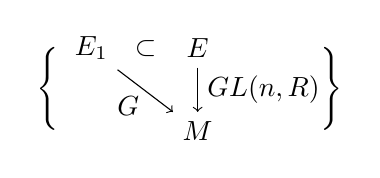
\begin{tikzpicture}[baseline=(E.base),x=1cm,y=1cm]
 \node (Eone) at (0,0) {$E_1$};
 \node at (.69,0) {$\subset$};
 \node (E) at (1.35,0) {$E$};
 \node (M) at (1.35,-1.05) {$M$};
 \draw[->] (Eone.south east) -- node[below left,inner sep=2pt] {$G$} (M.north west);
 \draw[->] (E) -- node[right] {$GL(n,R)$} (M);
 \node at (-.55,-.52) {$\Biggl\{$};
 \node at (3.05,-.52) {$\Biggr\}$};
\end{tikzpicture}}\endgroup}
\end{GelfandAdjacentEvidence}
\begin{GelfandAdjacentEvidence}{GELFAND-P000922}{3}


\underline{Задача:} [зачёркнуто] рассмотреть все геометрии на $S^2$, связанные с различными подгруппами $G\subset GL(n,R)$.
\Unclear{GELFAND-P000922}{cancelled-task-word}{Слово перед «рассмотреть» зачёркнуто и не читается.}
\end{GelfandAdjacentEvidence}
\begin{GelfandAdjacentEvidence}{GELFAND-P000922}{4}


\uuline{Д. Б. Фукс.}\quad\underline{О когомологиях по Делиню, Макферсону и т.д.}

\hspace{2em}\uuline{по Макферсону.}

$X$ --- мн-зие с особ., т.е. есть стратификация
\begin{equation*}
 X=X_n\supset X_{n-1}\supset\ldots\supset X_0.
 \tag{1}
\end{equation*}

$X_i-X_{i-1}$ --- гладкое $2i$-мерное мн-зие

и нек-рое естеств. условие лок. тривиальности

\SourceFigure{GELFAND-P000922}{stratum}{Рисунок к условию локальной тривиальности.%
\par\smallskip
\begingroup\color{black}\GelfandFitDiagram{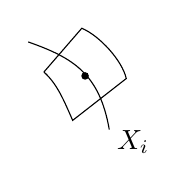
\begin{tikzpicture}[scale=.83]
 \draw (.31,1.01) -- (.89,1.68)
    .. controls (1.17,1.56) and (1.51,1.18) .. (1.57,.91)
    -- (.75,.27) .. controls (.61,.59) and (.51,.83) .. (.31,1.01);
 \draw (.07,1.47) .. controls (.75,1.23) and (1.16,.99) .. (1.31,.13);
 \fill (.94,.95) circle (.058);
 \node[anchor=north west,inner sep=0pt] at (1.42,.12) {$X_i$};
\end{tikzpicture}}\endgroup}
\end{GelfandAdjacentEvidence}
\begin{GelfandAdjacentEvidence}{GELFAND-P000922}{5}


Точка $x_0\in X_i$ имеет такую окр. $U$, что

в стратификации
\begin{equation*}
 U\supset U\cap X_{n-1}\supset U\cap X_{n-1}\supset\ldots\supset U\cap X_i
 \tag{2}
\end{equation*}
[зачёркнуто: «диффеоморфна» (?) […] «стратификации» (?)]

во всех точках $U\cap X_i$ устроена одинаково
\SourceFigure{GELFAND-P000922}{stratification-repeated-index}{В (2) два раза подряд написано $U\cap X_{n-1}$.}
\end{GelfandAdjacentEvidence}
\begin{GelfandAdjacentEvidence}{GELFAND-P000922}{6}

\Incomplete{GELFAND-P000922}{cancelled-local-triviality}{Середина зачёркнутой строки не читается. Начало и конец приведены предположительно.}
\end{GelfandAdjacentEvidence}
\begin{GelfandAdjacentEvidence}{GELFAND-P000922}{7}


Рассм. циклы из [обведено и вписано сверху: синг.] симплексов $\sigma^q$, для к-рых
\begin{equation*}
 \dim(\sigma^q\cap X_{n-i})\leq q-i
 \qquad (\operatorname{Codim}X_{n-i}=2i\,!)
 \tag{3}
\end{equation*}

(как то усл., к-рое было бы, если бы было общее полож. с выд. частью)

Если справа $q$ или $q-2i$ (!), то получ. обычные когомологии.

Фактор по [зачёркнуто сверху] гр. от цепей, на к-рые наложено аналог. условие.
\Unclear{GELFAND-P000922}{correction-above-boundaries}{Зачёркнутый знак перед «гр.» не читается.}
\end{GelfandAdjacentEvidence}


\uwave{Другое опр., гипотетически эквив. этому}

Делинь хотел, чтобы годилось над кон. полями.

более спец. причина: есть надежда док. связ. с $L^2$-когомологиями

($L^2$ [вписано снизу: -формы] при подх. к страту)

\underline{А. Бейлинсон.}\quad Опред. выше можно придать лок. вид (перейти к комплексу пучков, его когом. будут когом. Макферсона).


\Needspace{7\baselineskip}
\begin{GelfandAdjacentEvidence}{GELFAND-P000923}{1}
\SourcePage{GELFAND-P000923}{unlabelled}

Сейчас то же с исп. дифф. операторов

Вложим
\[
 X\hookrightarrow\underset{\text{мн-зие [без особенностей]}}{Y}
\]
\begin{equation*}
 X_{\mathrm{reg}}=X_n-X_{n-1}\hookrightarrow X\hookrightarrow Y.
 \tag{4}
\end{equation*}

На $X_n-X_{n-1}$ рассм. трив. сис. д. у., т.е.

пучок $\mathcal O_{X_{\mathrm{reg}}}$ --- пучок ф-й, он же пучок мод. над кольцом дифф. опер.

Хотим продолжить это на всё $Y$.

\underline{Пример:}

$X$ --- крест, \qquad $Y$ --- плоскость
\SourceFigure{GELFAND-P000923}{example-cross-left-point}{Четыре стрелки направлены внутрь. Слева от левой стрелки есть отдельная точка, принадлежность которой к рисунку неясна.%
\par\smallskip
\begingroup\color{black}\GelfandFitDiagram{\begin{tikzpicture}[scale=.8]
 \draw[->] (-1.53,.03) .. controls (-1.0,.10) and (-.62,.07) .. (-.14,.02);
 \draw[->] (1.09,-.02) -- (.13,-.02);
 \draw[->] (.08,1.02) -- (.01,.13);
 \draw[->] (-.18,-.97) -- (-.07,-.12);
 \fill (-1.67,.02) circle (.026);
\end{tikzpicture}}\endgroup}
\end{GelfandAdjacentEvidence}
\begin{GelfandAdjacentEvidence}{GELFAND-P000923}{2}


продолж. ф-и, тензорно умножая на $\delta$ по трансверсали

На них действуют дифф. операторы.

(и в общ. случае так)

Вдоль $X$ должны быть регул. (и сосред. на $X$).

Рассм. пучок
\begin{equation*}
 U\longrightarrow\text{все сеч. над}\;(Y-X_{\mathrm{sing}})\;\text{постр. пучка}.
\end{equation*}
\SourceFigure{GELFAND-P000923}{sheaf-sections-domain}{После «над» записано $(Y-X_{\mathrm{sing}})$ без пересечения с $U$.}
\end{GelfandAdjacentEvidence}
\begin{GelfandAdjacentEvidence}{GELFAND-P000923}{3}


(5)\quad (прямой образ в смысле теор. пучков при влож. $\underline{Y-X_{\mathrm{sing}}\overset{i}{\hookrightarrow}Y}.$)

(6)\quad \underline{Теор. 1.}

В этом пучке мод. есть \uwave{единств. неприв. подмодуль}!

(\underline{Мораль} (И.М.Г.) в теории особ. надо работать с дифф. операторами.)

Итак, строится модуль над кольцом дифф. опер. над $Y$.

(пучок модулей)

На $X_{\mathrm{reg}}$ рассм. пучок ф-и и прод. их $\delta$-ф-ями в трансверс. напр.

Получ. на $Y\setminus X_{\mathrm{sing}}$ модуль над дифф. опер. (с голом. или алгебр. коэфф.)
\Unclear{GELFAND-P000923}{overwritten-sing-index}{Индекс в этой строке переписан поверх другого начертания. Итоговое чтение «sing».}
\end{GelfandAdjacentEvidence}
\begin{GelfandAdjacentEvidence}{GELFAND-P000923}{4}


\uwave{Продолжаем в особенность} $X_{\mathrm{sing}}$.

Модуль стр. в 2 шага

\underline{1 шаг.} Максим. --- прямой образ пучка.

\underline{2 шаг.} Берём неприв. подмодуль (он единственен!!)

\underline{Здесь:} регулярные вдоль $X$, но без согласования!
\SourceFigure{GELFAND-P000923}{cross-four-limits}{(4 разных предела!)%
\par\smallskip
\begingroup\color{black}\GelfandFitDiagram{\begin{tikzpicture}[scale=.72]
 \draw (-.84,0) -- (.96,.03);
 \draw (-.15,-.8) .. controls (-.10,-.43) and (.12,.39) .. (.05,.73);
 \fill (0,.014) circle (.064);
\end{tikzpicture}}\endgroup}
\end{GelfandAdjacentEvidence}
\begin{GelfandAdjacentEvidence}{GELFAND-P000923}{5}


[зачёркнуто сверху] Рассм. резольвенту этого модуля $M$
\Incomplete{GELFAND-P000923}{cancelled-resolution-word}{Слово над «резольвенту» густо зачёркнуто и не читается.}
\end{GelfandAdjacentEvidence}
\begin{GelfandAdjacentEvidence}{GELFAND-P000923}{6}

\begin{equation*}
 \ldots\longrightarrow F_1\longrightarrow F_0\longrightarrow M\longrightarrow0
 \tag{7}
\end{equation*}

($F_j$ --- своб. мод. над дифф. опер. [зачёркнуто] $\mathcal D_Y$)
\Unclear{GELFAND-P000923}{cancelled-ring-symbol}{Зачёркнутый знак перед $\mathcal D_Y$ не читается.}
\end{GelfandAdjacentEvidence}


и отобр. в ф-и над $Y$ (в $\mathcal O_Y$)


\Needspace{7\baselineskip}
\begin{GelfandAdjacentEvidence}{GELFAND-P000924}{1}
\SourcePage{GELFAND-P000924}{7}

\[\bullet\longrightarrow F_1\longrightarrow F_0\longrightarrow M\longrightarrow0\]

Возн. комплекс:
\begin{equation*}
 \operatorname{Hom}_{\mathcal D}(F_0,\mathcal O_Y)
 \longrightarrow \operatorname{Hom}_{\mathcal D}(F_1,\mathcal O_Y)
 \longrightarrow\ldots
 \tag{8}
\end{equation*}
\SourceFigure{GELFAND-P000924}{complex-verb-letter}{Сокращение перед «комплекс» читается «Возн.».}
\end{GelfandAdjacentEvidence}
\begin{GelfandAdjacentEvidence}{GELFAND-P000924}{2}


до $\operatorname{Codim}_Y X$ это \uwave{ациклично}, а дальше Макферс. когомологии

(9)\quad \uwave{Простейшие переопр. сист. д. у.} --- те, у к-рых лок. сущ. $\max$ кол-во

(10)\quad решений (привод. к системе $\dfrac{\partial u}{\partial x_1}=0,\ldots,\dfrac{\partial u}{\partial x_n}=0$) --- они цел. (?) опр. сист.

своих реш. --- будет лок. пост. пучок на мн-зии.
\Unclear{GELFAND-P000924}{systems-abbreviation}{После «они» предположительно написано «цел.».}
\end{GelfandAdjacentEvidence}
\begin{GelfandAdjacentEvidence}{GELFAND-P000924}{3}


Реш. лок. --- $\mathrm{const}$.

Глобальных реш. может не быть

Аналог в общей сит.

Рассм. любую переопр. сист.

(11)\quad Если сист. имеет \uwave{рег. особенности} (есть опред.), то решения ---

--- Макферс. комплекс.
\SourceFigure{GELFAND-P000924}{fuchsian-annotation}{Приписка справа. Стрелка указывает на «рег. особенности» в (11).%
\par\smallskip
\(\uparrow\)\enspace обобщ. пон. фуксовой сист.}
\end{GelfandAdjacentEvidence}
\begin{GelfandAdjacentEvidence}{GELFAND-P000924}{4}


Это устанав. соотв. между этими компл. и сист. с рег. особ.

\underline{Определение} (\underline{Кашивара}) \uwave{сист. с рег. особ.}

Классич. опред. (для сист. обыкн. ур-й) --- рег. особ. (Фуксова сист.):
\begin{equation*}
 \frac{dx}{dt}=\frac1t A(t)x,\quad\text{где }A\text{ регул}.
 \tag{12}
\end{equation*}
(сист. 1-го порядка)

Пусть [зачёркнуто] дан $\mathcal D$-модуль $M$ (связ. с переопр. сист.)
\Unclear{GELFAND-P000924}{cancelled-before-module}{Зачёркнутое перед «дан» не читается.}
\end{GelfandAdjacentEvidence}
\begin{GelfandAdjacentEvidence}{GELFAND-P000924}{5}


(13)\quad а) Пусть $M$ не имеет кручения, т.е. если $x\in M$, $x\ne0$,

$f\in\mathcal D$, $f\ne0$, то $fx\ne0$.
\SourceFigure{GELFAND-P000924}{torsion-ring}{Буква в $f\in\mathcal D$ совпадает по начертанию с $\mathcal D$ в строке о модуле.}
\end{GelfandAdjacentEvidence}
\begin{GelfandAdjacentEvidence}{GELFAND-P000924}{6}

\SourceFigure{GELFAND-P000924}{torsion-margin}{Справа: (нет ничего, сидящего вдоль мн-зий)}
\end{GelfandAdjacentEvidence}
\begin{GelfandAdjacentEvidence}{GELFAND-P000924}{7}


[зачёркнуто: Тогда […] треб., чтобы суж. вдоль дост. рег. кривой име[…] вид (12)]
\Incomplete{GELFAND-P000924}{cancelled-restriction-word}{После «Тогда» густо зачёркнутое слово не читается.}
\end{GelfandAdjacentEvidence}
\begin{GelfandAdjacentEvidence}{GELFAND-P000924}{8}

\Incomplete{GELFAND-P000924}{cancelled-restriction-ending}{Перед «вид (12)» различимо начало «име-».}
\end{GelfandAdjacentEvidence}
\begin{GelfandAdjacentEvidence}{GELFAND-P000924}{9}


(14)\quad Тогда она прив. к сист. (10)

(15)\quad \underline{Утв.} У $M$ рег. особ. $\Longleftrightarrow$ суж. вдоль дост. рег. кривой имеет вид (12)
\SourceFigure{GELFAND-P000924}{assertion-restriction}{После знака эквивалентности читается «суж.», как и в зачёркнутой строке выше.}
\end{GelfandAdjacentEvidence}
\begin{GelfandAdjacentEvidence}{GELFAND-P000924}{10}


\underline{Общее опр.} В $\forall$ модуле есть фильтрация

(конечная длина!) и неприв. факторы имеет вид (10) ---

--- интегр. связность.
\SourceFigure{GELFAND-P000924}{filtration-verb}{В строке о факторах читается «имеет» в единственном числе.}
\end{GelfandAdjacentEvidence}


\underline{Опр.} Каждая неприв. компон. должна иметь регул. особ.


\Needspace{7\baselineskip}
\begin{GelfandAdjacentEvidence}{GELFAND-P000925}{1}
\SourcePage{GELFAND-P000925}{unlabelled}

\underline{27.10.80}\qquad\uuline{Сем. Гельфанда.}

\dotuline{Задачи (для первокурсников)}

1.\enspace Найти все подгруппы и норм. подгруппы группы (?) симметрии правильных многогранников и симметрической группы.
\Unclear{GELFAND-P000925}{task1-group-ending}{Окончание слова перед «симметрии» густо переписано. По управлению возможно «группы», но окончание не читается.}
\end{GelfandAdjacentEvidence}
\begin{GelfandAdjacentEvidence}{GELFAND-P000925}{2}


2.\enspace Односвязна ли группа $SL(2,R)$? Построить её универ. накрывающую.
\begin{gather*}
 \alpha\delta-\beta\gamma=1
 \;\Longleftrightarrow\;
 \alpha_1^2-\alpha_2^2-\alpha_3^2+\alpha_4^2=1\\
 \Longleftrightarrow\;
 \alpha_1^2+\alpha_4^2=1+\alpha_2^2+\alpha_3^2
 \;\Longleftrightarrow\\
 \Longleftrightarrow\;
 \left(\underbrace{\frac{\alpha_1}{\sqrt{1+\alpha_2^2+\alpha_3^2}}}_{x_1}\right)^2+
 \left(\underbrace{\frac{\alpha_4}{\sqrt{1+\alpha_2^2+\alpha_3^2}}}_{x_2}\right)^2=1.
\end{gather*}
\Unclear{GELFAND-P000925}{circle-index-corrections}{Индексы $3$ в первом знаменателе, $4$ во втором числителе и $2$ во втором знаменателе переписаны. Первоначальные знаки неразборчивы.}
\end{GelfandAdjacentEvidence}


\[
 \underset{\text{гомотопич. эквив.}}{(\alpha_1,\alpha_2,\alpha_3,\alpha_4)}
 \longmapsto (x_1,x_2)\in S^1
\]

Точнее, получается
\[
 SL(2,R)\underset{\text{диффеом.}}{\cong} S^1\times R^2.
\]

3.\enspace Как устроена универ. накр. $SL(2,R)$ как группа?


\Needspace{7\baselineskip}
\begin{GelfandAdjacentEvidence}{GELFAND-P000926}{1}
\SourcePage{GELFAND-P000926}{unlabelled}

Пусть есть 3 прямые
\SourceFigure{GELFAND-P000926}{three-lines}{Три прямые с метками $\ell_1,\ell_2,\ell_3$.%
\par\smallskip
\begingroup\color{black}\GelfandFitDiagram{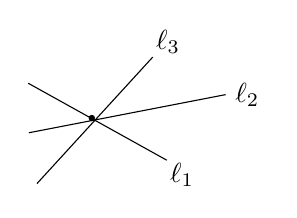
\begin{tikzpicture}[scale=.85]
 \draw (-.95,.52) -- (1.12,-.63) node[below right,inner sep=1pt] {$\ell_1$};
 \draw (-.94,-.22) -- (2.0,.35) node[right] {$\ell_2$};
 \draw (-.82,-.98) -- (.91,.91) node[above right,inner sep=1pt] {$\ell_3$};
 \fill (0,0) circle (.048);
\end{tikzpicture}}\endgroup}
\end{GelfandAdjacentEvidence}
\begin{GelfandAdjacentEvidence}{GELFAND-P000926}{2}

\[
 [?](\ell_1,\ell_2,\ell_3)=
 \begin{cases}
 +1 & \text{если $\ell_2$ внутри угла $\widehat{\ell_1\ell_3}$ (угол $<\pi$).}\\
 -1 & \text{в противн. случае}
 \end{cases}
\]
\Unclear{GELFAND-P000926}{triple-sign-name}{Знак перед аргументами сильно обведён. Возможны $\tau$ и $f$. В правой приписке трёхместная функция обозначена $f$.}
\end{GelfandAdjacentEvidence}
\begin{GelfandAdjacentEvidence}{GELFAND-P000926}{3}


$(g_j,n_j)$ --- элемент, $g_j\in SL(2,C)$
\SourceFigure{GELFAND-P000926}{group-field}{В этой строке написано $C$. На предыдущем листе в вопросе 3 стоит $R$.}
\end{GelfandAdjacentEvidence}
\begin{GelfandAdjacentEvidence}{GELFAND-P000926}{4}


\[
 (g_1,n_1)(g_2,n_2)=(g_1g_2,n_1+n_2+\tau(g_1,g_2))
\]
[зачёркнуто $\tau(\ell_1,g_1\ell_2,g_1g_2\ell_3)$; над формулой вписано $\tau(g_1,g_2)$.]
\Incomplete{GELFAND-P000926}{product-cancellation}{После $n_1+n_2+$ имеется также более густо зачёркнутая запись. Её чтение не установлено.}
\end{GelfandAdjacentEvidence}
\begin{GelfandAdjacentEvidence}{GELFAND-P000926}{5}


$(\ell_1,\ell_2,\ell_3)$ можно выб. произвольно, приводя к гомолог. коциклу
\begin{gather*}
 g=\begin{pmatrix}\alpha&\beta\\0&\alpha^{-1}\end{pmatrix}
 \qquad
 \varphi(g)=\begin{cases}1,&\alpha>0\\-1,&\alpha<0\end{cases}\\[4pt]
 g=\begin{pmatrix}a&b\\c&d\end{pmatrix}
 \qquad
 \varphi(g)=\begin{cases}i&c>0\\-i&c<0\end{cases}
\end{gather*}
(если не прив. к треуг.)
\[
 \varphi(g,n)=e^{i\frac{\pi}{2}n}\varphi(g)
\]
\SourceFigure{GELFAND-P000926}{scalar-function-name}{Буква $\varphi$ в формуле с экспонентой имеет ту же петлю, что и в двух формулах выше и в определении $\widetilde G$.}
\end{GelfandAdjacentEvidence}
\begin{GelfandAdjacentEvidence}{GELFAND-P000926}{6}


Теперь надо взять
\[
 \widetilde G=\{(g,n):\varphi(g,n)=1\}
\]
$\widetilde G$ --- это группа и она есть универ. накрывающая.

\medskip
[справа]
(Здесь $\ell_3=\ell$ --- ось $X$)
\[
 \tau(g_1,g_2)=f(\ell,g_1\ell\,g_1g_2\ell)=\pm1
\]
\Unclear{GELFAND-P000926}{triple-argument-divider}{Между вторым и третьим аргументами отдельная запятая не различается.}
\end{GelfandAdjacentEvidence}
\begin{GelfandAdjacentEvidence}{GELFAND-P000926}{7}


$\ell$ --- направл. прямая

(инвар. тройки [вписано снизу, обведено: направл.] прямых; индекс тройки прямых;
\SourceFigure{GELFAND-P000926}{directed-insertion}{Сокращение «направл.» обведено и подведено к первому «прямых».}
\end{GelfandAdjacentEvidence}
\begin{GelfandAdjacentEvidence}{GELFAND-P000926}{8}


$+1$ если $g_1\ell$ между $\ell$ и $g_1g_2\ell$

\uwave{Эта гр. несвязна} --- есть 4 куска; тогда надо взять связн. комп.

4.\enspace (Кириллов). Описать все локально проективные структуры на $R$

(покр. картами, переход --- дробно-лин. преобр.)

атласы эквив., если переход --- др.-лин. преобр.

\underline{Ответ}: есть счетное число лок. проект. структур

\uwave{1 пример}. $R$ и пар. $t$

\uwave{2 пример}:
\SourceFigure{GELFAND-P000926}{projective-charts}{Две верхние оси $t$, $s$ с нулями и нижняя ось $x$.%
\par\smallskip
\begingroup\color{black}\GelfandFitDiagram{\begin{tikzpicture}[scale=.64]
 \draw[<->] (0,0) -- (2.1,0);
 \draw (1.04,-.08) -- (1.04,.09);
 \node at (.96,.28) {$t$};
 \node at (1.18,-.28) {$0$};
 \draw[<->] (2.92,0) -- (4.49,0);
 \draw (3.65,-.08) -- (3.65,.09);
 \node at (3.69,.28) {$s$};
 \node at (3.82,-.28) {$0$};
 \node[anchor=west,inner sep=0pt] at (4.78,0) {--- настоящие};
 \draw[<->] (1.5,-.91) -- (3.5,-.91);
 \draw (2.48,-1.01) -- (2.48,-.82);
 \node at (2.65,-1.2) {$x$};
\end{tikzpicture}}\endgroup}
\end{GelfandAdjacentEvidence}
\begin{GelfandAdjacentEvidence}{GELFAND-P000926}{9}


\dotuline{Соотн.:} $tx=-1,\quad xs=-1$

Кончилась одна --- пер. к другой и т.д.

2-я не эквив. 1-й.

2-листное накр. на проект. прямую имеет лок. проект. структуру.

Накр. проект. прямой --- её проект. преобр. будут --- обр. универс. накрытия.

\uuline{Проф. Гаво} (\uwave{из Парижа})\qquad\underline{3 возм. темы.}
\SourceFigure{GELFAND-P000926}{paris-arrow}{Приписка над строкой с выноской к «из Парижа».%
\par\smallskip
\(\leftarrow\)\enspace\underline{Univ. Paris VI}}
\end{GelfandAdjacentEvidence}
\begin{GelfandAdjacentEvidence}{GELFAND-P000926}{10}


1.\enspace Констр. оболочек голоморфности

2.\enspace Констр. мер на нек-рых $\infty$-мерн. однор. мн-зиях

3.\enspace Теория рассеяния и функц. интегралы.
\SourceFigure{GELFAND-P000926}{gaveau-marginal}{Справа: Гаво --- ученик Маллевена, к-рый сейчас заним. случайной дифф. геометрией.}
\end{GelfandAdjacentEvidence}
\begin{GelfandAdjacentEvidence}{GELFAND-P000926}{11}


1.\enspace\dotuline{О конструкциях оболочек голоморфности.}

Рассм. $C^2$ и попробуем постр. обол. голом. комп. 2-мерной пов. (в $C^2$)

\uuline{Зад.} Найти такую [зачёркнуто] Леви-плоскую гиперпов. $M$, такую что
\[
 \partial M=S^2
\]
(форма Леви на ней должна быть $=0$)
\Incomplete{GELFAND-P000926}{levi-cancellation}{Слово перед «Леви-плоскую» густо зачёркнуто и не читается.}
\end{GelfandAdjacentEvidence}
\begin{GelfandAdjacentEvidence}{GELFAND-P000926}{12}


Леви плоская обл. рассл. на компл. слои

(На торе эту зад. решить нельзя)
\SourceFigure{GELFAND-P000926}{levi-foliation}{На верхнем краю овала короткий тёмный штрих, направление которого неясно.%
\par\smallskip
\begingroup\color{black}\GelfandFitDiagram{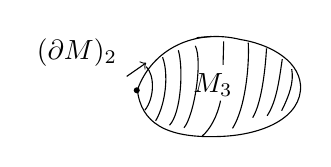
\begin{tikzpicture}[scale=.80]
 \draw (-1.22,-.03)
 .. controls (-.99,.62) and (-.31,.95) .. (.42,.77)
 .. controls (.81,.71) and (1.33,.48) .. (1.37,.05)
 .. controls (1.40,-.47) and (.76,-.76) .. (.03,-.77)
 .. controls (-.77,-.79) and (-1.16,-.55) .. cycle;
 \draw (-1.08,.34) .. controls (-.94,.20) and (-.95,-.16) .. (-1.10,-.35);
 \draw (-.82,.49) .. controls (-.72,.22) and (-.77,-.25) .. (-.93,-.52);
 \draw (-.57,.60) .. controls (-.49,.33) and (-.52,-.39) .. (-.71,-.59);
 \draw (-.30,.67) .. controls (-.18,.42) and (-.32,-.44) .. (-.48,-.63);
 \draw (.15,.74) -- (.14,.37);
 \draw (.10,-.20) .. controls (.05,-.45) and (-.07,-.66) .. (-.19,-.76);
 \draw (.54,.72) .. controls (.56,.39) and (.50,-.31) .. (.29,-.64);
 \draw (.83,.63) .. controls (.81,.28) and (.75,-.24) .. (.61,-.47);
 \draw (1.08,.46) .. controls (1.03,.12) and (.99,-.21) .. (.84,-.44);
 \draw (1.23,.30) .. controls (1.27,.09) and (1.18,-.14) .. (1.07,-.36);
 \draw (-.28,.80) -- (-.04,.82);
 \fill (-1.23,-.035) circle (.048);
 \node at (-.02,.05) {$M_3$};
 \node (boundary) at (-2.18,.56) {$(\partial M)_2$};
 \draw[->] (boundary.south east) -- (-1.08,.40);
\end{tikzpicture}}\endgroup%
\par\dotuline{покрытие дисками} (слоение)}
\end{GelfandAdjacentEvidence}



\Needspace{7\baselineskip}
\begin{GelfandAdjacentEvidence}{GELFAND-P000927}{1}
\SourcePage{GELFAND-P000927}{11}

Есть особ. точки слоения $\Rightarrow$ индекс вырожд. (?) зад. Римана $=0$ $\Rightarrow$ она решается
\Unclear{GELFAND-P000927}{top-index-abbreviation}{Сокращение перед «зад. Римана» предположительно «вырожд.» или «вырож.».}
\end{GelfandAdjacentEvidence}
\begin{GelfandAdjacentEvidence}{GELFAND-P000927}{2}


(Бишоп --- \underline{возник.} \underline{синг.} интегро-дифф. ур-е)

\underline{2-3}.

$M$ --- мн-зие, $G$ --- комп. гр. Ли; $g$ --- алг. Ли

$\Lambda^1(M,g)$ --- 1-формы на $M$ со знач. в $g$.
\Unclear{GELFAND-P000927}{forms-cancelled-index}{Нижний индекс у $\Lambda$ зачёркнут. Возможна цифра $2$.}
\end{GelfandAdjacentEvidence}
\begin{GelfandAdjacentEvidence}{GELFAND-P000927}{3}

\SourceFigure{GELFAND-P000927}{yang-mills-margin}{На правом поле: «хотим квантовать Янга-Миллса».}
\end{GelfandAdjacentEvidence}
\begin{GelfandAdjacentEvidence}{GELFAND-P000927}{4}


\begin{equation*}
 e^{-\int_M\operatorname{Tr}(\Omega\Omega)}D(\omega)
 \tag{1}
\end{equation*}
\SourceFigure{GELFAND-P000927}{curvature-annotations}{Под формулой (1) подписаны кривизна и связность.%
\par\smallskip
\begingroup\color{black}\GelfandFitDiagram{\begin{tikzpicture}[scale=.77]
 \node (Omega) at (0,0) {$\Omega$};
 \node (omega) at (2.03,0) {$\omega$};
 \node (curv) at (0,-.88) {кривизна \(\omega\)};
 \node (conn) at (2.67,-.88) {связность};
 \draw[->] (curv) -- (Omega);
 \draw (omega.south east) -- (conn.north west);
\end{tikzpicture}}\endgroup}
\end{GelfandAdjacentEvidence}
\begin{GelfandAdjacentEvidence}{GELFAND-P000927}{5}


(Формальный фейнман. интеграл)

\uwave{Группа:} $g\in C(M,G)$ (калибр.)
\begin{equation*}
 g\cdot\omega=g^{-1}dg+g^{-1}\omega g
 \tag{2}
\end{equation*}
\Incomplete{GELFAND-P000927}{gauge-cancellation}{Сразу после второго $g^{-1}$ зачёркнуто выражение, которое не удаётся прочесть.}
\end{GelfandAdjacentEvidence}
\begin{GelfandAdjacentEvidence}{GELFAND-P000927}{6}


Цель --- построить инвар. меру отн. \dotuline{калибр.} [зачёркнуто] \underline{группы}.
\Unclear{GELFAND-P000927}{group-word-cancellation}{Перед «группы» зачёркнута короткая запись. Возможно, «гр.».}
\end{GelfandAdjacentEvidence}
\begin{GelfandAdjacentEvidence}{GELFAND-P000927}{7}


(проще, чем на факторпр-ве)

Надо интегр. по мн-ву траекторий в $\Lambda^1$.
\begin{equation*}
 e^{-\int_0^t dt\int_M\operatorname{Tr}(\Omega_t\Omega_t)\,dx}D(\omega_t).
 \tag{3}
\end{equation*}

Будем построено семейство мер, «приближ.» к равнов. мере.
\SourceFigure{GELFAND-P000927}{measure-family-verb}{Читается «Будем построено». Первое слово имеет окончание «м», второе --- «ено».}
\end{GelfandAdjacentEvidence}
\begin{GelfandAdjacentEvidence}{GELFAND-P000927}{8}

\SourceFigure{GELFAND-P000927}{gauge-orbit-figure}{Орбиты, точка $\Pi$ и две линии, выходящие из неё.%
\par\smallskip
\begingroup\color{black}\GelfandFitDiagram{\begin{tikzpicture}[scale=.73]
 \draw[densely dotted] (.25,-.82) .. controls (-.01,-.45) and (-.03,.35) .. (.24,.90);
 \draw (.16,.12) -- (.10,-.10);
 \draw (.60,-.86) .. controls (.34,-.38) and (.35,.44) .. (.59,.92);
 \draw (1.01,-.88) .. controls (.78,-.35) and (.82,.47) .. (1.02,.89);
 \draw (1.45,-.87) .. controls (1.17,-.43) and (1.22,.39) .. (1.47,.83);
 \fill (.10,-.10) circle (.045);
 \node[anchor=east,inner sep=2pt] at (.05,.21) {$\Pi$};
 \draw[thick] (.10,-.10) -- (1.66,-.07);
 \draw (.10,-.10) .. controls (.31,.17) and (.40,.08) .. (.56,.17)
 .. controls (.68,.30) and (.79,.21) .. (.91,.27) -- (1.25,.44);
 \draw (1.71,.64) -- (2.02,.78);
 \node[anchor=west,align=left,inner sep=1pt] at (2.14,.79) {\scriptsize орбиты калибр. гр.};
 \draw (1.69,-.20) -- (2.03,-.39);
 \node[anchor=west,align=left,inner sep=1pt] at (2.14,-.41) {\scriptsize трансверс. сеч.};
\end{tikzpicture}}\endgroup}
\end{GelfandAdjacentEvidence}
\begin{GelfandAdjacentEvidence}{GELFAND-P000927}{9}


\uwave{Сначала} --- типа винер. меры на путях.

Нужно что-то вроде эллипт. оператора в пр-ве связностей, инвар. отн. калибр. группы.
\[
 \Pi\to d_\Pi\text{ --- ковар. диффер.},\qquad
 \Box_\Pi=d_\Pi^*d_\Pi+d_\Pi d_\Pi^*
\]
\begin{equation*}
 e^{-\tau\Box_\Pi}(x,y)=p_\tau^{(\Pi)}(x,y)
 \qquad\text{--- \uuline{символ} функц.}
 \tag{4}
\end{equation*}
\SourceFigure{GELFAND-P000927}{heat-word}{После (4) дважды подчёркнуто слово «символ».}
\end{GelfandAdjacentEvidence}
\begin{GelfandAdjacentEvidence}{GELFAND-P000927}{10}

\begin{equation*}
 L\varphi(\Pi)=\iint_{M\times M} e^{-\tau\Box_\Pi}(x,y)
 \frac{\delta^2\varphi}{\delta\Pi(x)\delta\Pi(y)}\,dx\,dy
 \tag{5}
\end{equation*}

[зачёркнуто] \uwave{\(\tau\) фиксирован}.
\Incomplete{GELFAND-P000927}{fixed-tau-cancellation}{Перед $\tau$ знак или короткое слово зачёркнуто. Чтение не установлено.}
\end{GelfandAdjacentEvidence}


Нельзя раб. в соб. пр-вах.
\begin{equation*}
 \Lambda^1_{k,\alpha}(M,g),\quad 0<\alpha<1,
 \tag{6}
\end{equation*}
--- какое-то пр-во (гёльдеровское)

$k$-я пр. им. гёльд. на $\alpha$.

Нужно:
\begin{equation*}
 \left\|e^{-\tau\Box_\Pi}-e^{-\tau\Box_{\Pi'}}\right\|_{HS}
 \le C\|\Pi-\Pi'\|
 \tag{7}
\end{equation*}
[под \(HS\): Гильб.-Шмидта.]


\Needspace{7\baselineskip}
\begin{GelfandAdjacentEvidence}{GELFAND-P000928}{1}
\SourcePage{GELFAND-P000928}{unlabelled}

Получается
\begin{equation*}
 \left\|e^{-\tau\Box_\Pi}-e^{-\tau\Box_{\Pi'}}\right\|_{HS(L^2,L^2)}
 \le C\|\Pi-\Pi'\|_{k,\alpha}
 \tag{8}
\end{equation*}
\SourceFigure{GELFAND-P000928}{eq8-bound}{В (8) под знаком $<$ есть косой штрих. Читается $\le$.}
\end{GelfandAdjacentEvidence}
\begin{GelfandAdjacentEvidence}{GELFAND-P000928}{2}


Технич. мом.: броуновское движ. выводит из пр-ва, $e^{-\tau\Box_\Pi}$ возвращает обратно.
\SourceFigure{GELFAND-P000928}{space-phrase}{Перед экспонентой читается «выводит из пр-ва».}
\end{GelfandAdjacentEvidence}
\begin{GelfandAdjacentEvidence}{GELFAND-P000928}{3}

\begin{equation*}
 d\Pi_t=e^{-\tau\Box_\tau}\underbrace{d\beta_t}_{\text{белый шум}}.
 \tag{9}
\end{equation*}
\SourceFigure{GELFAND-P000928}{equation09-index}{В (9) индекс у $\Box$ той же формы, что и стоящее перед $\Box$ $\tau$.}
\end{GelfandAdjacentEvidence}
\begin{GelfandAdjacentEvidence}{GELFAND-P000928}{4}


[зачёркнуто: \sout{Интересно}]
\SourceFigure{GELFAND-P000928}{cancelled-interesting}{Над (10) зачёркнуто слово «Интересно».}
\end{GelfandAdjacentEvidence}
\begin{GelfandAdjacentEvidence}{GELFAND-P000928}{5}

\begin{equation*}
 \left(\tfrac12\Delta-V\right)\Psi=\frac{\partial}{\partial t}\Psi
 \tag{10}
\end{equation*}
\begin{equation*}
 \Psi_t(x)=E_x\left(\exp\left(-\int_0^t V(b_\omega(s))\,ds\right)
 \Psi_0(b_\omega(t))\right)
 \tag{11}
\end{equation*}

В частности,
\begin{equation*}
 \pm\lambda_1=\lim_{t\to\infty}
 \frac{\log E_x\bigl(\exp\bigl(-\int_0^t V(b_\omega(s))\,ds\bigr)}{t}
 \tag{12}
\end{equation*}
\SourceFigure{GELFAND-P000928}{equation12-parentheses}{В числителе (12) после $ds$ только одна закрывающая скобка.}
\end{GelfandAdjacentEvidence}
\begin{GelfandAdjacentEvidence}{GELFAND-P000928}{6}


(Интересно, напр., когда есть отриц. уровни)

Пусть
\begin{equation*}
 \left|\Delta^{-1}V\right|\le C<1
 \tag{13}
\end{equation*}
\Unclear{GELFAND-P000928}{equation13-operator}{Знак перед $^{-1}$ переписан. Внешний контур читается как $\Delta$, а прежний знак не установлен.}
\end{GelfandAdjacentEvidence}
\begin{GelfandAdjacentEvidence}{GELFAND-P000928}{7}


Тогда
\begin{equation*}
 E_x\left(\exp\left(-\int_0^\infty V(b_\omega(s))\,ds\right)\right)
 \le\frac{1}{1-C}
 \tag{14}
\end{equation*}
\Unclear{GELFAND-P000928}{equation14-path}{Буква в (14) переписана. Принято чтение $b_\omega$ по (11)–(12), но возможно $B_\omega$.}
\end{GelfandAdjacentEvidence}
\begin{GelfandAdjacentEvidence}{GELFAND-P000928}{8}


$\Rightarrow$ оценив. соб. значение.
\SourceFigure{GELFAND-P000928}{eigenvalue-word}{После «соб.» читается «значение».}
\end{GelfandAdjacentEvidence}
\begin{GelfandAdjacentEvidence}{GELFAND-P000928}{9}


$V\longmapsto\varepsilon V$\quad пот. (?) взяли $\varepsilon$ мало $\Rightarrow$ что-то оценивается.
\Unclear{GELFAND-P000928}{last-line-abbreviation}{Сокращение после $\varepsilon V$ неясно. Возможно «пот.» (потенциал).}
\end{GelfandAdjacentEvidence}



\Needspace{7\baselineskip}
\begin{GelfandAdjacentEvidence}{GELFAND-P000929}{1}
\SourcePage{GELFAND-P000929}{unlabelled}

\uuline{3/$\overline{\underline{\mathrm{XI}}}$-80 г.}
\qquad \underline{Сем.} \underline{Гельфанда.}

\underline{И.М.Г.}\qquad \underline{История теории представлений}

1.\enspace Дедекинд --- характеры конечн. коммут. групп (для $L$-ф-ий)

2.\enspace Фробениус --- матрицы и следы для некоммут. групп

3.\enspace Хаар (рано умер)

(*)4.\enspace фон Нейман --- теория $C^*$-алгебр для предст. некоммут. групп

(**)5.\enspace Гельфанд и Наймарк --- о предст. гр. Лоренца

\uwave{Идеология} (*): всё устроено теоретико-множественно

\hspace{2em}(**). ---\(//\)--- гладко и просто

Совр. анализ: некоммут. дифф. геометрия и интегр. геометрия.

{\small Надо учит. гладкую структуру.}
\SourceFigure{GELFAND-P000929}{inserted-structure}{В тесной строке после «учит.» читается «гладкую». Начало слова подчёркнуто коротким штрихом.}
\end{GelfandAdjacentEvidence}
\begin{GelfandAdjacentEvidence}{GELFAND-P000929}{2}


Групп. алгебра для алг. Ли --- \uwave{оберт. алгебра.}

но: их всё равно много (нет теор. Веддербарна)
\SourceFigure{GELFAND-P000929}{wedderburn-name}{Фамилия в рукописи написана «Веддербарна».}
\end{GelfandAdjacentEvidence}
\begin{GelfandAdjacentEvidence}{GELFAND-P000929}{3}


\uwave{Гельфанд, Кириллов.}\enspace тело отнош. оберт. алг. \(\cong\) тело отнош. кольца дифф. операторов

Это не доделано. (Недостаточно опер. с полин. коэффициентами; частично это понято в раб. [зачёркнуто] Новикова, Кричевера, Шабата и т.п.)
\Unclear{GELFAND-P000929}{cancelled-before-novikov}{Помета перед «Новикова» густо зачёркнута и не читается.}
\end{GelfandAdjacentEvidence}
\begin{GelfandAdjacentEvidence}{GELFAND-P000929}{4}


\uwave{Бернштейн, С. Гельфанд, И.М. Гельфанд}\qquad в проект. пр-ве.

Надо раб. с пучками.

Сейчас уже надо прислушивать (?) не теорию предст., а то, для чего она делается.
\Unclear{GELFAND-P000929}{last-line-verb}{Начальные штрихи глагола допускают чтения «прислушивать» и «прослушивать».}
\end{GelfandAdjacentEvidence}



\Needspace{7\baselineskip}
\begin{GelfandAdjacentEvidence}{GELFAND-P000930}{1}
\SourcePage{GELFAND-P000930}{16}

\underline{А. Бейлинсон}

$X$ --- алгебр. мн-зие над $\mathbb C$

Самые простые --- аффинные.

Они однозн. опред. кольцом ф-й на них.

\uwave{Коммут. кольцо} $=$ [зачёркнуто: алгеб. (?)] \uwave{аффинное алг. мн-зие.}
\Unclear{GELFAND-P000930}{cancelled-affine-word}{Зачёркнутое после знака равенства предположительно читается «алгеб.».}
\end{GelfandAdjacentEvidence}
\begin{GelfandAdjacentEvidence}{GELFAND-P000930}{2}


\uwave{Модули над ним} $=$ \uwave{квазикогер. пучки}

$X=\operatorname{Spec} A$, $M$ --- $A$-модуль (всегда топ. Зарисского)

базис откр. мн-в: \(X_f=\{x:f(x)\ne0\}\).

$O(X_f)=A_f$ --- локализация $A$ по $f$

\[
 \mathcal M(X_f)=M_f=M\otimes_A A_f
\]

Получ. пучок на $\operatorname{Spec} A$. Так получ. класс квазикогер. пучков на $X$.

\uwave{Будет некоммут. аналог локализации}. (переход от мод. к пучку).

(1)\quad \underline{Кольца:} \uwave{универс. оберт. алг. полупр. алг. Ли и их факторы.}

$X$ --- алг. мн. --- наз. $\mathcal D$-\uwave{аффинным}, если оно облад. св-вом

($\mathcal D_X$ --- пучок колец дифф. опер. на $X$)

$X$ --- гладкое;
\SourceFigure{GELFAND-P000930}{smooth-assumption}{Слева у строки о гладкости: «Счит., что».}
\end{GelfandAdjacentEvidence}
\begin{GelfandAdjacentEvidence}{GELFAND-P000930}{3}


$\mathcal M$ --- пучок модулей над $\mathcal D_X$, $O_X\subset\mathcal D_X$ (подпучок; дифф. опер. 0-го пор.)

$\mathcal M$ наз. \uwave{квазикогерентным}, если он квазиког. как пучок $O_X$-модулей.

(\underline{Пример}: сам $\mathcal D_X$ квазикогерентен).

$X$ --- алгебр. мн-зие, $O_X$ --- пучок ф-й на нём; пучок $\mathcal M$ $O_X$-модулей на $X$

наз. \uwave{квазикогерентным}, если он облад. след. св-вом:

\(\forall\) аффинного мн-ва $U$ и его афф. подмн-ва \(U'\subset U\) должно быть:
\begin{equation*}
 \mathcal M(U')=\mathcal M(U)\otimes_{O(U)}O(U')
 \tag{2}
\end{equation*}

(ясно, что правая часть (2) отобр. в левую, треб., чтобы это было изоморфизмом)

(3)\quad \underline{Утверждение}. $X$ аффинно \(\Longleftrightarrow\) \(\forall\) квазикогер. $\mathcal M$

(4)\quad \(\underset{i>0}{H^i(X,\mathcal M)=0}\) и $\mathcal M$ порожд. над $O(X)$ глоб. сечениями, т.е.
\SourceFigure{GELFAND-P000930}{generation-ring}{В (4) написано $O(X)$. В следующей строке под знаком тензорного произведения кольцо не указано.}
\end{GelfandAdjacentEvidence}


\begin{equation*}
 H^0(X,\mathcal M)\otimes O_X
 \underset{\text{\uwave{эпиморфизм}}}{\longrightarrow}\mathcal M
 \tag{5}
\end{equation*}

(Не совсем трив. теорема --- Серр, Гротендик --- см. раб. Серра о когер. пучках)


\Needspace{7\baselineskip}
\begin{GelfandAdjacentEvidence}{GELFAND-P000931}{1}
\SourcePage{GELFAND-P000931}{unlabelled}

(6).\quad \underline{Определение}. $X$ наз. $\mathcal D$-\uwave{аффинным}, если $\forall$ квазикогер. пучка $\mathcal D$-модулей $\mathcal M$ вып. условия (4), (5), т.е.
\Incomplete{GELFAND-P000931}{cancelled-before-7}{Слева от (7) зачёркнута прежняя метка. Похожа на (8), но чтение не установлено.}
\end{GelfandAdjacentEvidence}
\begin{GelfandAdjacentEvidence}{GELFAND-P000931}{2}

\begin{equation*}
 H^i(X,\mathcal M)=0,\quad i>0
 \tag{7}
\end{equation*}
\begin{equation*}
 H^0(X,\mathcal M)\otimes\mathcal D_X\longrightarrow\mathcal M\longrightarrow0
 \tag{8}
\end{equation*}

(9)\quad \underline{Примеры}.

1.\enspace $\forall$ афф. мн-зие --- $\mathcal D$-аффинно.

2.\enspace $\forall$ проект. пр-во $\mathbb P^N$ --- $\mathcal D$-аффинно.

(частн. случай теор., о к-рой будет идти речь)

3.\enspace Эллипт. кривая --- не $\mathcal D$-аффинно.

(10)\quad \uwave{Следствие} $\mathcal D$-\uwave{аффинности}

Пусть $X$ --- мн-зие, $\mathcal L$ --- пучок $O$-модулей, рассмотрим

(11)\quad $\mathcal D_X\otimes_{O_X}\mathcal L$ --- квазикогер. пучок $\mathcal D_X$-модулей

[зачёркнуто сверху]
(12)\quad $X$ --- $\mathcal D$-афф. \(\Rightarrow\) когомологии пучка (11) равны $0$ и он порожд. глоб. сеч. (т.е. вып. (7) и (8)), даже если сам $\mathcal L$ был плохой
\Incomplete{GELFAND-P000931}{cancelled-above-12}{Над началом (12) зачёркнуто короткое слово, которое не удаётся прочесть.}
\end{GelfandAdjacentEvidence}
\begin{GelfandAdjacentEvidence}{GELFAND-P000931}{3}


(13)\quad (например, $O(-i)$ на $\mathbb P^N$, он не имеет сечений и имеет высшие когомологии)
\SourceFigure{GELFAND-P000931}{twist-index-13}{У густо обведённой буквы видна точка. Читается $i$.}
\end{GelfandAdjacentEvidence}
\begin{GelfandAdjacentEvidence}{GELFAND-P000931}{4}


\hspace{2em}{\small например,}

(14)\quad $\mathcal D_X\otimes_{O_X}O(-i)$ на $P^N$ порожд. глоб. сечениями
\SourceFigure{GELFAND-P000931}{twist-index-14}{В (14) снова $O(-i)$, с обведённой буквой $i$.}
\end{GelfandAdjacentEvidence}
\begin{GelfandAdjacentEvidence}{GELFAND-P000931}{5}


(докладчик не знает прямого док-ва)

К сожалению, нет хорошей записи $\mathcal D_X$, т.к. дифф. опер. глобально не записывается в виде суммы однородных.

(14) --- некий лок. свободный $\mathcal D_X$-модуль.

$\mathcal D_X$ в (11) рассматривается как правый пучок $O_X$-модулей
\Unclear{GELFAND-P000931}{overwritten-reference}{Последняя цифра ссылки на (11) сильно обведена.}
\end{GelfandAdjacentEvidence}
\begin{GelfandAdjacentEvidence}{GELFAND-P000931}{6}


Если рассмотреть
\begin{equation*}
 O(-i)\otimes_{O_X}\mathcal D_X,
 \tag{15}
\end{equation*}
то это будет уже не так; он не порожд. глоб. сеч. и высш. когом. $\ne0$ ($O(-i)$ --- его прямое слагаемое)

[зачёркнуто: \sout{Эллипт. кривая}]\qquad\underline{Об эллипт. кривой}.
\SourceFigure{GELFAND-P000931}{cancelled-elliptic-title}{Перед новым заголовком прежний зачёркнут.}
\end{GelfandAdjacentEvidence}
\begin{GelfandAdjacentEvidence}{GELFAND-P000931}{7}


(16)\quad Пусть на $\mathcal D_X$ есть инволюция, тожд. на $O_X$, и \(ab\overset{*}{\mapsto}ba\);
\SourceFigure{GELFAND-P000931}{involution-product}{Над стрелкой между $ab$ и $ba$ стоит звёздочка.}
\end{GelfandAdjacentEvidence}
\begin{GelfandAdjacentEvidence}{GELFAND-P000931}{8}


тогда (14) и (15) были бы изоморфны и мн-зие не было бы $\mathcal D$-афф.

Но на элл. кривой есть \uwave{инволюция} --- взятие формально сопр. оператора
\[
 f\cdot\frac{\partial}{\partial x}\mapsto\frac{\partial}{\partial x}f
\]
\SourceFigure{GELFAND-P000931}{formal-adjoint-sign}{Перед дробью справа в рукописи не видно знака минуса.}
\end{GelfandAdjacentEvidence}
\begin{GelfandAdjacentEvidence}{GELFAND-P000931}{9}


(есть коорд. --- все опер. «с пост. коэфф.»)
\SourceFigure{GELFAND-P000931}{last-parenthesis}{В начале скобок читается «есть коорд.».}
\end{GelfandAdjacentEvidence}



\Needspace{7\baselineskip}
\begin{GelfandAdjacentEvidence}{GELFAND-P000932}{1}
\SourcePage{GELFAND-P000932}{17}

От $\mathcal D_X$ отщепляется кольцо ф-й $\Rightarrow$ (15) не ациклично
\Unclear{GELFAND-P000932}{opening-reference}{Первая цифра в ссылке обведена. По связи с предыдущим кадром читается (15).}
\end{GelfandAdjacentEvidence}
\begin{GelfandAdjacentEvidence}{GELFAND-P000932}{2}


(17)\quad \underline{Утверждение}. $X$ --- \underline{$\mathcal D$-аффинно}, \underline{тогда}
[зачёркнутая запись не разобрана] \underline{функтор сечений} $\Gamma$
\begin{equation*}
 \mathcal D_X\text{-mod}\overset{\Gamma}{\longrightarrow}\Gamma(\mathcal D_X)\text{-mod},
 \tag{18}
\end{equation*}
\underline{является эквивалентностью категорий}.
\Incomplete{GELFAND-P000932}{line17-cancel}{Одно зачёркнутое слово между «тогда» и «функтор» не разобрано.}
\end{GelfandAdjacentEvidence}
\begin{GelfandAdjacentEvidence}{GELFAND-P000932}{3}


(Докладчик не знает, вытекает ли отсюда $\mathcal D$-аффинность; в коммут. случае это так)
\Unclear{GELFAND-P000932}{note-after-speaker}{После «Докладчик» стоит маленький густо обведённый знак. Его роль не установлена.}
\end{GelfandAdjacentEvidence}
\begin{GelfandAdjacentEvidence}{GELFAND-P000932}{4}


\begin{equation*}
 D_X\underset{\mathrm{def}}{=}\Gamma(\mathcal D_X)
 \tag{19}
\end{equation*}

[зачёркнуто: \sout{Теорема} (?)]
\Unclear{GELFAND-P000932}{before20-cancel}{Перед (20) зачёркнута запись, похожая на «Теорема».}
\end{GelfandAdjacentEvidence}
\begin{GelfandAdjacentEvidence}{GELFAND-P000932}{5}


(20)\quad Достат. условие не $\mathcal D$-аффинности --- [зачёркнутая запись не разобрана] $ch_1$ (пучка форм. макс. степени) $=0$
\SourceFigure{GELFAND-P000932}{condition20-scope}{В заголовке между «не» и $\mathcal D$ дефиса не видно.}
\end{GelfandAdjacentEvidence}
\begin{GelfandAdjacentEvidence}{GELFAND-P000932}{6}

\Incomplete{GELFAND-P000932}{line20-cancel}{Зачёркнутая запись перед $ch_1$ не разобрана.}
\end{GelfandAdjacentEvidence}
\begin{GelfandAdjacentEvidence}{GELFAND-P000932}{7}

\begin{equation*}
 \bigl(\Leftrightarrow ch_1(\text{касат. рассл.})=0\bigr)
 \tag{21}
\end{equation*}
\begin{equation*}
 (20)\Leftrightarrow(21)\Leftrightarrow\text{сущ. инволюции.}
 \tag{22}
\end{equation*}

(Дифф. опер. с перест. $x$ и $\frac{\partial}{\partial x}$ --- дифф. опер. на формах max степ.)

\textit{[межстрочная вставка:]} Изом. обр. пучков $\Leftrightarrow ch_1$ совпадают

(23)\quad \underline{Теорема}. $G$ --- \underline{полупр. группа} [вписано сверху и обведено: алг. (?)] Ли,
$B$ --- \underline{борелевская подгр.},
\underline{рассм.} $X=G/B$ --- («пр-во флагов»). \underline{тогда}
[зачёркнуто: \sout{\mbox{$X$ --- $\mathcal D$-аффинно и}}]
\Unclear{GELFAND-P000932}{insert-circled-word}{Обведённая вставка похожа на «алг.». Указатель идёт вниз к «группа Ли». Точное чтение не установлено.}
\end{GelfandAdjacentEvidence}
\begin{GelfandAdjacentEvidence}{GELFAND-P000932}{8}

\SourceFigure{GELFAND-P000932}{theorem-cancel}{После «Тогда» зачёркнуто «$X$ --- $\mathcal D$-аффинно и».}
\end{GelfandAdjacentEvidence}
\begin{GelfandAdjacentEvidence}{GELFAND-P000932}{9}


1.\enspace $X$ --- $\mathcal D$-аффинно

2.\enspace $D_X=U(\mathfrak g)/U(\mathfrak g)I_0$;

\begin{quote}
\textit{[на правом поле, слева квадратная скобка]}

(*) ([зачёркнутая запись не разобрана])

\underline{Пример:} $G=SL(2,\mathbb C)$,

$B$ --- треуг.

$G/B=\mathbb P^1$

какие дифф. опер. на $\mathbb P^1$?
\end{quote}
\Incomplete{GELFAND-P000932}{example-cancel}{Запись в скобках перед «Пример» зачёркнута. Точное чтение не установлено.}
\end{GelfandAdjacentEvidence}
\begin{GelfandAdjacentEvidence}{GELFAND-P000932}{10}


где
\SourceFigure{GELFAND-P000932}{central-character}{Диаграмма (24). Между $Z(\mathfrak g)$ и $U(\mathfrak g)$ стоит знак, похожий на $\cap$.%
\par\smallskip
\begingroup\color{black}\GelfandFitDiagram{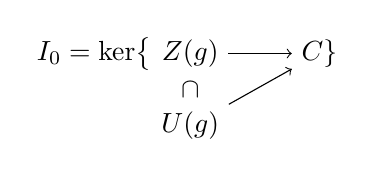
\begin{tikzpicture}[baseline=(z.base)]
\node (i) at (-1.22,0) {$I_0=\ker\bigl\{$};
\node (z) at (0,0) {$Z(\mathfrak g)$};
\node (c) at (1.64,0) {$\mathbb C\}$};
\node (u) at (0,-0.92) {$U(\mathfrak g)$};
\node at (0,-0.46) {$\cap$};
\draw[->] (z) -- (c);
\draw[->] (u) -- (c);
\end{tikzpicture}}\endgroup
\par (24)\quad --- станд. единств. одном. характер}
\end{GelfandAdjacentEvidence}
\begin{GelfandAdjacentEvidence}{GELFAND-P000932}{11}


$I_0$ --- операторы Лапласа без своб. члена

[зачёркнуто: \sout{Утверждение} (?)] \underline{Предложение}.
\Unclear{GELFAND-P000932}{before25-cancel}{Зачёркнутое слово перед «Предложение» похоже на «Утверждение».}
\end{GelfandAdjacentEvidence}
\begin{GelfandAdjacentEvidence}{GELFAND-P000932}{12}


(25)\quad \underline{$D_X$-модули} $\Leftrightarrow$ \underline{представления} $\mathfrak g$,
\underline{на к-рых трив. действует} $I_0$.

($Z(\mathfrak g)$ должно действ. как на трив. 1-мерном представлении)

\underline{Пример (*).}

(26)\quad На $\mathbb P^1$ есть [вписано сверху: дифф.] опер.
\SourceFigure{GELFAND-P000932}{projective-operators}{Три оператора в (26) объединены нижней скобкой. К «опер.» ведёт дуга от вписанного «дифф.».%
\par\smallskip
\begingroup\color{black}\GelfandFitDiagram{\begin{tikzpicture}
\node (operators) {$\dfrac{d}{dx},\quad x\dfrac{d}{dx}\quad\text{и}\quad x^2\dfrac{d}{dx}$};
\draw (operators.south west) -- ++(0,-0.12) -| (operators.south east);
\end{tikzpicture}}\endgroup}
\end{GelfandAdjacentEvidence}
\begin{GelfandAdjacentEvidence}{GELFAND-P000932}{13}

Берутся полиномы от них --- это обёрт. алгебра.

Есть единств. опер., перест. со всеми. (Шварцман?)
\Unclear{GELFAND-P000932}{last-name}{Предположительное чтение фамилии «Шварцман». Знак вопроса есть в рукописи.}
\end{GelfandAdjacentEvidence}


\underline{Мораль:} теория представлений сводится к теории $\mathcal D_X$-модулей.

\underline{Улучшение по ср. с известным:} можно локализовать!!

\Needspace{7\baselineskip}
\begin{GelfandAdjacentEvidence}{GELFAND-P000933}{1}
\SourcePage{GELFAND-P000933}{unlabelled}

\underline{\underline{10.11.80 г.}}\qquad\underline{Сем. Гельфанда.}
\Unclear{GELFAND-P000933}{above-date-marks}{Над датой несколько отдельных штрихов. Буквы или цифры не различимы.}
\end{GelfandAdjacentEvidence}
\begin{GelfandAdjacentEvidence}{GELFAND-P000933}{2}


\underline{И. М. Г.}\qquad\underline{\underline{Числа Кэли.}}
\begin{equation*}
 \left|\sum_{j=1}^{8}x_j e_j\right|=\sqrt{\sum_{1}^{8}x_j^2}
 \tag{1}
\end{equation*}
\Unclear{GELFAND-P000933}{formula1-overwritten-number}{Слева от цифры в (1) густой переписанный или зачёркнутый штрих. Прежний знак не установлен.}
\end{GelfandAdjacentEvidence}
\begin{GelfandAdjacentEvidence}{GELFAND-P000933}{3}

\Unclear{GELFAND-P000933}{right-sum-upper-limit}{Под чертой корня верхний предел соприкасается с чертой. Читается предположительно $8$, по сопоставлению с левой частью.}
\end{GelfandAdjacentEvidence}
\begin{GelfandAdjacentEvidence}{GELFAND-P000933}{4}


В числах Кэли:
\begin{equation*}
 |ab|=|a||b|
 \tag{2}
\end{equation*}

Как док., что нет $>8$ измер.?

Получ. задача из теории предст. благодаря (2) и явная конструкция.

\underline{Вопрос:} \uwave{может быть, бывает в $\infty$-мерном пр-ве?} (с усл. (2))

Гиндикин утв., что бывает. Надо повторить док-во того, что в конечномерном случае ничего не бывает, кроме $\mathbb R,\mathbb C,\mathbb H$ и Кэли.

Проективные геометрии (плоскости).

Ввод. координаты, ассоциативность $\Leftrightarrow$ дезарговость

Проект. плоскость Кэли --- простейшая \uwave{недезаргова}

Интересно изучить диффер. и лок. однородные проект. плоскости.

--- Зад. классиф. алгебр Ли --- слишком частная (надо, чтобы не было обрывков

\hfill $G_2,E_6,E_7,E_8$ и т.п.
\SourceFigure{GELFAND-P000933}{exceptional-types}{Ряд типов записан под «надо, чтобы не было обрывков». Закрывающей скобки не видно.}
\end{GelfandAdjacentEvidence}
\begin{GelfandAdjacentEvidence}{GELFAND-P000933}{5}


\underline{\underline{Бейлинсон.}}\qquad\underline{О локализации представлений.}

$X$ --- алг. мн-зие (над $\mathbb C$),

$\mathcal A$ --- квазикогерентный $O_X$-модуль

\hspace{2em}\(\vert\) пучок колец, содержащий $O_X$.
\SourceFigure{GELFAND-P000933}{sheaf-vertical-mark}{От $\mathcal A$ вниз к следующей строке идёт короткий вертикальный штрих.}
\end{GelfandAdjacentEvidence}
\begin{GelfandAdjacentEvidence}{GELFAND-P000933}{6}


(включение $O_X\subset\mathcal A$ [вписано снизу: задано])
\SourceFigure{GELFAND-P000933}{inclusion-insertion}{«Задано» вписано под знаком включения.}
\end{GelfandAdjacentEvidence}


(Напр., $\mathcal A$ --- пучок дифф. операторов)

\uwave{$\mathcal A$-mod} --- \uwave{категория пучков левых} $\mathcal A$-\uwave{мод.},
\uwave{явл. квазикогер.} $O_X$-\uwave{модулями}

\Needspace{7\baselineskip}
\begin{GelfandAdjacentEvidence}{GELFAND-P000934}{1}
\SourcePage{GELFAND-P000934}{20}

(В прошлый раз было $\mathcal A$ --- дифф. опер.)

$A=\Gamma(\mathcal A)$,\qquad $A$-mod --- катег. $A$-модулей (левых).

Есть 2 сопр. функтора.
\SourceFigure{GELFAND-P000934}{adjunction-arrows}{В (1) стрелка $\Gamma$ идёт вправо, дуга $\Delta$ под ней --- влево.%
\par\smallskip
\begingroup\color{black}\GelfandFitDiagram{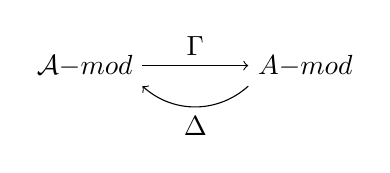
\begin{tikzpicture}[baseline=(sheaves.base)]
\node (sheaves) at (0,0) {$\mathcal A\text{-mod}$};
\node (modules) at (2.8,0) {$A\text{-mod}$};
\draw[->] (sheaves.east) -- node[above] {$\Gamma$} (modules.west);
\draw[->] (modules.south west) to[bend left=42] node[below] {$\Delta$} (sheaves.south east);
\end{tikzpicture}}\endgroup
\par (1)}
\end{GelfandAdjacentEvidence}
\begin{GelfandAdjacentEvidence}{GELFAND-P000934}{2}


\begin{equation*}
 \Delta(M)=\mathcal A\mathbin{\underset{A}{\otimes}}M,
 \tag{2}
\end{equation*}
$M$ рассм. как пост. пучок $\mathcal A$-мод. над $X$
(слой $=M$ над каждой точкой) и отобр. тривиальны.
\SourceFigure{GELFAND-P000934}{tensor-over-A}{В (2) $A$ записано прямо под знаком тензорного произведения.}
\end{GelfandAdjacentEvidence}
\begin{GelfandAdjacentEvidence}{GELFAND-P000934}{3}

\SourceFigure{GELFAND-P000934}{constant-module-notation}{Перед «мод. над $X$» стоит каллиграфическая $\mathcal A$, как слева в (1).}
\end{GelfandAdjacentEvidence}
\begin{GelfandAdjacentEvidence}{GELFAND-P000934}{4}


Легко видеть, что они сопряжены.

(3)\quad \underline{Опред.-лемма.} [зачёркнуто: \sout{а)} (?)]
\Unclear{GELFAND-P000934}{definition-cancel}{Знак после заголовка зачёркнут. Возможно, «а)».}
\end{GelfandAdjacentEvidence}
\begin{GelfandAdjacentEvidence}{GELFAND-P000934}{5}


\uwave{Мн-зие} $X$ \uwave{наз.} $\mathcal A$-\uwave{аффинным}, \uwave{если вып. одно из 2-х эквив. условий}

а)\enspace $\forall\,\mathcal M\in\mathcal A\text{-mod},\quad H^i(X,\mathcal M)=0,\quad i>0$ и
\[
 \begin{gathered}
 H^0(X,\mathcal M)\ne0\\[-2pt]
 \text{при }\mathcal M\ne0
 \end{gathered}
\]

б)\enspace \uwave{Функторы} $\Gamma$ и $\Delta$ \uwave{являются взаимно-обратными эквивалентностями категорий}.

(На самом деле а) эквив. тому, что было в прошлый раз, меняем модули)

а) нужно проверять, б) нужно использовать.
\SourceFigure{GELFAND-P000934}{need-check}{Перед «проверять» и «использовать» написано одно и то же слово «нужно».}
\end{GelfandAdjacentEvidence}
\begin{GelfandAdjacentEvidence}{GELFAND-P000934}{6}


\underline{Док-во эквивалентности а) и б).}

\underline{а) $\Rightarrow$ б).}
\begin{equation*}
 \Gamma(\mathcal M)=\operatorname{Hom}_{\mathcal A\text{-mod}}(\mathcal A,\mathcal M)
 \tag{4}
\end{equation*}
(образ $1$ --- сечение $\mathcal M$).

(5)\quad а) $\Rightarrow$ $\mathcal A$ --- проективная образующая в катег. $\mathcal A$-mod.

(6)\quad (такой объект, что i) $\operatorname{Hom}(\mathcal A,\mathcal M)$ --- \underline{точный} функтор

(7)\quad ii) $\forall$ ненулев. объекта $\mathcal M$;\enspace
$\operatorname{Hom}(\mathcal A,\mathcal M)\ne0$)

(из ацикличности вытекает i), а из 2-го условия ii))

(точный функтор --- перев. точные посл. в точные)
\Unclear{GELFAND-P000934}{above-exact}{Над концом «точный» стоит отдельный вертикальный штрих. Возможно, это восклицательный знак.}
\end{GelfandAdjacentEvidence}
\begin{GelfandAdjacentEvidence}{GELFAND-P000934}{7}


i)\enspace --- св-во проективности

ii)\enspace --- образующая

(кстати, ii) $\Rightarrow$ можем отобразить $\mathcal A$ в фактор $\mathcal M/\operatorname{Im}t$ и т.д.)
\SourceFigure{GELFAND-P000934}{quotient-symbol}{После $\operatorname{Im}$ в знаменателе читается $t$.}
\end{GelfandAdjacentEvidence}
\begin{GelfandAdjacentEvidence}{GELFAND-P000934}{8}


(8)\quad iii) $\Gamma$ перев. прямые суммы в прямые суммы.
\[
 \Gamma(\oplus_i\mathcal M_i)=\oplus\Gamma(\mathcal M_i)
\]
\Unclear{GELFAND-P000934}{direct-sum-index}{У левого знака прямой суммы есть маленький штрих, предположительно индекс $i$. У правого такого штриха не видно.}
\end{GelfandAdjacentEvidence}


\Needspace{7\baselineskip}
\begin{GelfandAdjacentEvidence}{GELFAND-P000935}{1}
\SourcePage{GELFAND-P000935}{unlabelled}

(св-во любых квазиког. пучков)

\underline{Общекатег. факт}

(9)\quad \underline{Лемма.} Пусть зад. $\forall$ категория $C$ (абелева)
[вписано сверху: с прямыми суммами в $\forall$ кол-ве.], $X\in C$,
\SourceFigure{GELFAND-P000935}{direct-sums-insert}{Выноска от «(абелева)» ведёт к вставке о прямых суммах.}
\end{GelfandAdjacentEvidence}
\begin{GelfandAdjacentEvidence}{GELFAND-P000935}{2}


$X$ --- Проект. образующая со св-вом (8):
\Unclear{GELFAND-P000935}{overwritten-X}{$X$ в начале строки сильно обведён. Что было под ним, не установлено.}
\end{GelfandAdjacentEvidence}
\begin{GelfandAdjacentEvidence}{GELFAND-P000935}{3}


(10)\quad $\operatorname{Hom}_C(X,\cdot)$ коммут. с прямыми суммами.

(11)\quad [зачёркнуто: \sout{Тогда}]
\[
 \operatorname{Hom}_C(X,\cdot):C\longrightarrow\operatorname{End}_C X\text{-mod}
\]
\SourceFigure{GELFAND-P000935}{crossed-then}{Перед формулой (11) зачёркнуто «Тогда».}
\end{GelfandAdjacentEvidence}
\begin{GelfandAdjacentEvidence}{GELFAND-P000935}{4}


Тогда этот функтор --- \uwave{эквивал. категорий}.

Из леммы все вытекает, если применить её к случаю, когда
\begin{equation*}
 C=\mathcal A\text{-mod},\quad X=\mathcal A,\quad\operatorname{End}_C X=A
 \tag{12}
\end{equation*}
\SourceFigure{GELFAND-P000935}{endomorphism-ring}{Справа в (12) стоит $\operatorname{End}_C X=A$.}
\end{GelfandAdjacentEvidence}
\begin{GelfandAdjacentEvidence}{GELFAND-P000935}{5}


Обр. импликация \underline{б) $\Rightarrow$ а)} \underline{из} резольвенты Чеха.

$\mathcal D$-аффинное мн-зие, --- мн-зие, $\mathcal A$-афф. при $\mathcal A=\mathcal D_X$.

(13)\quad \underline{Теор.} $\mathbb P^N$ --- $\mathcal D$-\uwave{аффинно}.

Следующая теорема:
\SourceFigure{GELFAND-P000935}{theorem-heading}{Первое слово заголовка читается «Следующая».}
\end{GelfandAdjacentEvidence}
\begin{GelfandAdjacentEvidence}{GELFAND-P000935}{6}


$G$ --- редуктивная группа.

$X=G/B$ --- пр-во флагов

($B$ --- борелевская подгруппа)

(14)\quad $x\in X\Rightarrow\underset{\text{(стац.)}}{B_x}$ --- соотв. борелевская подгруппа
\SourceFigure{GELFAND-P000935}{stabilizer-note}{«(стац.)» вписано под $B_x$.}
\end{GelfandAdjacentEvidence}
\begin{GelfandAdjacentEvidence}{GELFAND-P000935}{7}


$G$ --- действ. на $X\Rightarrow\mathfrak g$ действ. на $X$.
\begin{equation*}
 \mathfrak g\longrightarrow\operatorname{Vect}X
 \tag{15}
\end{equation*}
\Unclear{GELFAND-P000935}{overwritten-15}{Вторая цифра в (15) сильно обведена, читается $5$.}
\end{GelfandAdjacentEvidence}
\begin{GelfandAdjacentEvidence}{GELFAND-P000935}{8}


отсюда.
\begin{equation*}
 U(\mathfrak g)\longrightarrow D_X=\Gamma(\mathcal D_X).
 \tag{16}
\end{equation*}

\SourceFigure{GELFAND-P000935}{center-leader}{Короткий загнутый штрих под $Z(\mathfrak g)$ рядом с пометой «центр».%
\par\smallskip
\begingroup\color{black}\GelfandFitDiagram{\begin{tikzpicture}[baseline=(z.base)]
\node (z) at (0,0) {$Z(\mathfrak g)\subset U(\mathfrak g)$};
\draw (-0.9,-0.27) .. controls (-0.99,-0.98) and (-0.65,-0.67) .. (-0.59,-0.25);
\draw (-0.40,-0.32) -- (-0.37,-0.47);
\node[anchor=west] at (-0.36,-0.58) {центр};
\end{tikzpicture}}\endgroup
\par (17)}
\end{GelfandAdjacentEvidence}
\begin{GelfandAdjacentEvidence}{GELFAND-P000935}{9}


$I$ --- аннулятор единичного предст. [?]
\Unclear{GELFAND-P000935}{annihilator-final-symbol}{Последний знак после «предст.» переписан. Точное чтение не установлено.}
\end{GelfandAdjacentEvidence}
\begin{GelfandAdjacentEvidence}{GELFAND-P000935}{10}


(max идеал в центре)
\begin{equation*}
 J=I\cdot U(\mathfrak g).
 \tag{18}
\end{equation*}

(19)\quad \underline{Теорема.} а) $X$ --- $\mathcal D$-\uwave{аффинно}.

б)\enspace \uwave{при морфизме} (16) \uwave{получается изоморфизм}
\begin{equation*}
 U(\mathfrak g)/J\overset{\sim}{\longrightarrow}D_X
 \tag{20}
\end{equation*}
\SourceFigure{GELFAND-P000935}{isomorphism-arrow}{В (20) одинарная стрелка с тильдой сверху.}
\end{GelfandAdjacentEvidence}


(21)\quad отсюда, эквив. категорий 1) $\mathcal D$-пучков на $X$ и 2) представлений алг. Ли $\mathfrak g$ с един. инфинитезим. характером.

\Needspace{7\baselineskip}
\begin{GelfandAdjacentEvidence}{GELFAND-P000936}{1}
\SourcePage{GELFAND-P000936}{21}

[зачёркнуто: \sout{Определение} (?)]\qquad\underline{Отступление.}
\Unclear{GELFAND-P000936}{cancelled-heading}{Зачёркнутый заголовок похож на «Определение». Точное чтение не установлено.}
\end{GelfandAdjacentEvidence}
\begin{GelfandAdjacentEvidence}{GELFAND-P000936}{2}

\SourceFigure{GELFAND-P000936}{section-heading}{Новый заголовок читается «Отступление».}
\end{GelfandAdjacentEvidence}
\begin{GelfandAdjacentEvidence}{GELFAND-P000936}{3}


$X,Y$ --- оба гладких алгебр. мн-зия.
\SourceFigure{GELFAND-P000936}{opening-word}{После $X,Y$ читается «оба».}
\end{GelfandAdjacentEvidence}
\begin{GelfandAdjacentEvidence}{GELFAND-P000936}{4}


$X\overset f\longrightarrow Y$ отображение.

Тогда имеются категории $\mathcal D_X\text{-mod}$ и $\mathcal D_Y\text{-mod}$

Есть 2 функтора в пучках $f^*$ и $f_*$.

Но в дифф. опер. нет никакого соответ. морфизма.

Но функторы (естеств.) есть, они опр. на уровне производной категории

(на самом деле есть \uwave{4 функтора})

(22)\quad $f^\circ$ --- обр. образ в кат. \underline{\underline{пучков}}.
\begin{equation*}
 O_X\mathbin{\underset{f^\circ O_Y}{\otimes}} f^\circ(\mathcal D_Y)
 \tag{23}
\end{equation*}
\SourceFigure{GELFAND-P000936}{inverse-image-23}{В (23) над $f$ видны маленькие незакрашенные кружки, как в (22).}
\end{GelfandAdjacentEvidence}
\begin{GelfandAdjacentEvidence}{GELFAND-P000936}{5}


\begin{equation*}
 \mathcal D_{X\to Y}\underset{\mathrm{def}}{=}
 O_X\mathbin{\underset{f^\bullet O_Y}{\otimes}} f^\bullet\mathcal D_Y
 \tag{24}
\end{equation*}
\SourceFigure{GELFAND-P000936}{inverse-image-24}{В (24) над обоими $f$ видны закрашенные точки.}
\end{GelfandAdjacentEvidence}
\begin{GelfandAdjacentEvidence}{GELFAND-P000936}{6}


\begin{equation*}
 \mathcal D_{X\to Y}\text{ --- }
 \left\{\begin{array}{l}
 \text{лев. } \mathcal D_X\text{-модуль}\\
 \text{прав. } f^\circ\mathcal D_Y\text{-модуль}
 \end{array}\right.
 \tag{25}
\end{equation*}
\SourceFigure{GELFAND-P000936}{transfer-bimodule}{В (25) знак над $f$ в нижней строке имеет незакрашенную середину.}
\end{GelfandAdjacentEvidence}
\begin{GelfandAdjacentEvidence}{GELFAND-P000936}{7}


лев. $\mathcal D_X$ по правилу Лейбница; ост. для вект. полей на $X$:
\SourceFigure{GELFAND-P000936}{leibniz-abbreviation}{После точки с запятой читается сокращение «ост.».}
\end{GelfandAdjacentEvidence}
\begin{GelfandAdjacentEvidence}{GELFAND-P000936}{8}


$v\in\operatorname{Vect}X$;
\[
 (df)(v)\in\Gamma(f^*T\,Y)
\]
\SourceFigure{GELFAND-P000936}{tangent-notation}{После $f^*$ написано $T$ и затем $Y$ на той же строке.}
\end{GelfandAdjacentEvidence}
\begin{GelfandAdjacentEvidence}{GELFAND-P000936}{9}


$(df)(v)$ действует на \underline{\underline{$f^\bullet\mathcal D_Y$}}.
\Unclear{GELFAND-P000936}{final-left-mark}{Слева от последней строки густой наклонный штрих. Отдельной точки под ним не видно.}
\end{GelfandAdjacentEvidence}
\begin{GelfandAdjacentEvidence}{GELFAND-P000936}{10}

\SourceFigure{GELFAND-P000936}{last-inverse-image}{Над $f$ стоит закрашенная точка. Запись дважды подчёркнута.}
\end{GelfandAdjacentEvidence}


\Needspace{7\baselineskip}
\begin{GelfandAdjacentEvidence}{GELFAND-P000937}{1}
\SourcePage{GELFAND-P000937}{unlabelled}

\underline{\underline{17.11.80 г.}}\qquad\underline{Сем. Гельфанда}

\underline{И. М. Г.}\qquad\underline{задачи.}

1.\quad
\[
 f(x)=\left\{\begin{array}{ll}
 1/q,&x=p/q\text{ --- несокр.}\\
 0,&x\text{ --- иррац.}
 \end{array}\right.
\]

Где она непрерывна?

где она дифференц.?
\[
 f(x)=\left\{\begin{array}{ll}
 1/q^\alpha,&x=p/q\text{ --- несокр.}\\
 0,&x\text{ --- иррац.}
 \end{array}\right.
\]

Что можно сказать о дифф.?

2.\quad $f(x)=\lim\limits_{n\to\infty}\lim\limits_{m\to\infty}(\cos^{2m}2\pi n!x)$ --- ф-я Дирихле.
\SourceFigure{GELFAND-P000937}{dirichlet-limits}{В аргументе косинуса после $n$ стоит факториал. Внутренний предел берётся по $m$.}
\end{GelfandAdjacentEvidence}
\begin{GelfandAdjacentEvidence}{GELFAND-P000937}{2}


3.\quad Можно ли построить ф-ю Дирихле с одним знаком предела?

(из непр. ф-й)

[справа вверху]

4.\quad Вычислить приближенно
\[
 \int_{-\infty}^{\infty}e^{-x^2}\cos1000x\,dx
\]

То же с $e^{-x^4}$ или $e^{-x^6}$
\SourceFigure{GELFAND-P000937}{upper-right-exercise}{Задача 4 записана в правом верхнем углу. В интеграле стоит $1000x$.}
\end{GelfandAdjacentEvidence}
\begin{GelfandAdjacentEvidence}{GELFAND-P000937}{3}


\underline{А. Бейлинсон.}

$X\overset f\longrightarrow Y$,\qquad $X,Y$ --- мн-зия.

$\mathcal D_X\text{-mod},\ \mathcal D_Y\text{-mod}$ --- категории квазикогер. пучков
$\mathcal D_X\text{-mod}$ и $\mathcal D_Y\text{-mod}$ на $X$ и $Y$
\SourceFigure{GELFAND-P000937}{functor-arrows}{Верхняя стрелка направлена вправо, нижняя влево. Меток над стрелками нет.%
\par\smallskip
\(\mathcal D_X\text{-mod}\ \substack{\longrightarrow\\\longleftarrow}\
\mathcal D_Y\text{-mod}\)\par функторы}
\end{GelfandAdjacentEvidence}
\begin{GelfandAdjacentEvidence}{GELFAND-P000937}{4}


Определим:
\[
 f^*:\mathcal D_Y\text{-mod}\longrightarrow\mathcal D_X\text{-mod}
\]
\begin{equation*}
 f^*(\mathcal M)=O_X\mathbin{\underset{f^\bullet(O_Y)}{\otimes}}
 f^\bullet(\mathcal M),\qquad \mathcal M\in\mathcal D_Y\text{-mod}
 \tag{1}
\end{equation*}

(как пучок --- \uwave{обр. образ в катег.} $O$-\uwave{модулей},
$f^\bullet$ --- абстрактный обратный образ)
\SourceFigure{GELFAND-P000937}{pullback-dots}{У обоих $f$ в правой части (1) стоят закрашенные точки. Звёздочка стоит слева.}
\end{GelfandAdjacentEvidence}
\begin{GelfandAdjacentEvidence}{GELFAND-P000937}{5}


Действие дифф. операторов: дост. вект. полей $v\in\operatorname{Vect}X$,
\begin{equation*}
 \ell\otimes m\in f^*(\mathcal M)
 \tag{2}
\end{equation*}
\SourceFigure{GELFAND-P000937}{tensor-factor-leaders}{Две выноски под множителями в (2).%
\par\smallskip
\begingroup\color{black}\GelfandFitDiagram{\begin{tikzpicture}[baseline=(l.base)]
\node (l) at (0,0) {$\ell$};
\node at (0.55,0) {$\otimes$};
\node (m) at (1.12,0) {$m$};
\node[anchor=west] at (1.5,0) {$\in f^*(\mathcal M)$};
\node (fn) at (-0.46,-0.82) {\scriptsize (ф-я на $X$)};
\node (sect) at (1.54,-0.82) {\scriptsize (сеч. $\mathcal M$)};
\draw (l.south) -- (fn.north east);
\draw (m.south) -- (sect.north west);
\end{tikzpicture}}\endgroup}
\end{GelfandAdjacentEvidence}
\begin{GelfandAdjacentEvidence}{GELFAND-P000937}{6}


\begin{equation*}
 df(v)=\sum
 \underset{\substack{\vert\\\text{ф-я на }X}}{\tau_i}
 \otimes\frac{\partial}{\partial y_i}\in f^*(T_Y),
 \qquad df:T_X\longrightarrow f^*T_Y
 \tag{3}
\end{equation*}
\SourceFigure{GELFAND-P000937}{tau-leader}{Под $\tau_i$ помета в единственном числе «ф-я на $X$».}
\end{GelfandAdjacentEvidence}
\begin{GelfandAdjacentEvidence}{GELFAND-P000937}{7}


Вместо (1) можно написать проще
\begin{equation*}
 f^*(\mathcal M)=O_X\mathbin{\underset{O_Y}{\otimes}}\mathcal M
 \tag{4}
\end{equation*}
В этом же смысле:
\begin{equation*}
 f^*(T_Y)=O_X\mathbin{\underset{O_Y}{\otimes}}T_Y
 \tag{5}
\end{equation*}
\begin{equation*}
 v\cdot(\ell\otimes m)\underset{\mathrm{def}}{=}
 v(\ell)\otimes m+\sum\ell\tau_i\otimes\frac{\partial}{\partial y_i}m
 \tag{6}
\end{equation*}
(по ф-ле Лейбница).
\SourceFigure{GELFAND-P000937}{leibniz-action}{Под равенством в (6) написано $\mathrm{def}$. Коэффициент в сумме читается $\ell\tau_i$.}
\end{GelfandAdjacentEvidence}


\Needspace{7\baselineskip}
\begin{GelfandAdjacentEvidence}{GELFAND-P000938}{1}
\SourcePage{GELFAND-P000938}{24}

Если $\mathcal M$ происх. из вект. рассл. с интегр. [вписано снизу: (плоской)] связностью, то это обычный обр. образ связности.
\SourceFigure{GELFAND-P000938}{flat-insert}{«(плоской)» вписано под «интегр.».}
\end{GelfandAdjacentEvidence}
\begin{GelfandAdjacentEvidence}{GELFAND-P000938}{2}


(7)\quad \underline{Примеры.}

1.\enspace $f^*O_Y=O_X$

2.\enspace Из пучка [зачёркнуто: знак не разобран] кон. типа может получ. [вписано сверху: пучок] бесконечного типа
\Incomplete{GELFAND-P000938}{example-two-cancel}{Густо зачёркнутый знак после «пучка». Возможно, $\mathcal D$.}
\end{GelfandAdjacentEvidence}
\begin{GelfandAdjacentEvidence}{GELFAND-P000938}{3}

\SourceFigure{GELFAND-P000938}{sheaf-insert}{«Пучок» вписано над строкой с выноской.}
\end{GelfandAdjacentEvidence}
\begin{GelfandAdjacentEvidence}{GELFAND-P000938}{4}


$X$ --- точка, $Y$ --- мн-зие.
\SourceFigure{GELFAND-P000938}{example-two-manifold}{После $Y$ читается сокращение «мн-зие».}
\end{GelfandAdjacentEvidence}
\begin{GelfandAdjacentEvidence}{GELFAND-P000938}{5}


$f^*(\mathcal D_Y)$ бесконечномерно (как вект. пр-во)
\[
 \mathcal D_X=\mathbb C
\]
$f^*(\mathcal D_Y)$ --- дифф. опер. с пост. коэффициентами

3.\enspace $X,Y$ как и выше, $\mathcal M$ --- $\delta$-ф-и в точке $X\in Y$
$\underset{\mathrm{def}}{=}\delta_x$

(обобщ. ф-и, соср. в точке).

Тогда
\[
 f^*(\delta_x)=0,
\]
т.к. $\forall$ обобщ. ф-ю [вписано сверху: в т.] можно предст. в виде
\[
 \sum \alpha_i s_i,\qquad \alpha_i(X)=0.
\]
\SourceFigure{GELFAND-P000938}{point-insert}{«в т.» вписано над строкой с выноской.}
\end{GelfandAdjacentEvidence}
\begin{GelfandAdjacentEvidence}{GELFAND-P000938}{6}


\SourceFigure{GELFAND-P000938}{delta-arrows}{От $y$ стрелка к $0$, от $\delta'(y)$ стрелка к «?».%
\par\smallskip
\begingroup\color{black}\GelfandFitDiagram{\begin{tikzpicture}[baseline=(ly.base)]
\node (ly) at (0,0) {$\delta(y)={}$};
\node (y) at (0.92,0) {$y$};
\node at (1.17,0) {$\cdot$};
\node (deriv) at (1.75,0) {$\delta'(y)$};
\node (zero) at (0.46,-0.90) {$0$};
\node (q) at (1.88,-0.90) {?};
\node[anchor=west] (reason) at (0.38,-1.57) {\scriptsize из-за замор… коэфф.};
\draw[->] (y.south) -- (zero.north east);
\draw[->] (deriv.south) -- (q.north);
\draw[->] (reason.north west) -- (zero.south);
\end{tikzpicture}}\endgroup}
\end{GelfandAdjacentEvidence}
\begin{GelfandAdjacentEvidence}{GELFAND-P000938}{7}

\SourceFigure{GELFAND-P000938}{delta-sign}{Перед $y$ написано равенство без видимого минуса.}
\end{GelfandAdjacentEvidence}
\begin{GelfandAdjacentEvidence}{GELFAND-P000938}{8}


\underline{Прямой образ} опр. для правых мод. (интегр. только формы!, а они --- правый мод.)

\[
 f_*\quad\text{mod-}\mathcal D_X\longrightarrow\text{mod-}\mathcal D_Y
\]
(интегрир. формы объёма на $X$ [вписано снизу и обведено: вдоль слоёв] даёт форму объёма на $Y$)
\SourceFigure{GELFAND-P000938}{fiber-insert}{Вставка «вдоль слоёв» обведена под строкой.}
\end{GelfandAdjacentEvidence}
\begin{GelfandAdjacentEvidence}{GELFAND-P000938}{9}


\begin{equation*}
 \underset{\substack{\vert\\\text{пучок на }X}}{\mathcal D_{X\to Y}}
 = f^*(\mathcal D_Y)\in\mathcal D_X\text{-mod-}\mathcal D_Y
 \tag{8}
\end{equation*}
\SourceFigure{GELFAND-P000938}{sheaf-on-x}{От обозначения пучка в (8) идёт вертикальная выноска вниз.}
\end{GelfandAdjacentEvidence}
\begin{GelfandAdjacentEvidence}{GELFAND-P000938}{10}


(левый $\mathcal D_X$-модуль и правый $\mathcal D_Y$-модуль)
\begin{equation*}
 f_*(\mathcal M)=f_{\cdot}\left(\mathcal M\mathbin{\underset{\mathcal D_X}{\otimes}}\mathcal D_{X\to Y}\right)
 \tag{9}
\end{equation*}
$f_{\cdot}$ --- прямой образ в пучках

[зачёркнуто: прежний номер не разобран] (10)\quad \underline{Примеры.}
\Unclear{GELFAND-P000938}{example-ten-cancel}{Перед (10) зачёркнут прежний номер. Его цифра не установлена.}
\end{GelfandAdjacentEvidence}
\begin{GelfandAdjacentEvidence}{GELFAND-P000938}{11}


1.\enspace $X=x\in Y$. Рассм. станд. 1-мерн. $\mathcal D_X$-модуль $(=\mathbb C)$
\SourceFigure{GELFAND-P000938}{standard-abbreviation}{Перед «1-мерн.» читается «станд.».}
\end{GelfandAdjacentEvidence}
\begin{GelfandAdjacentEvidence}{GELFAND-P000938}{12}

\[
 f_*(\mathcal M)\text{ --- (обобщ. ф-и, соср. в точке на }Y\text{)}=\delta_x
\]
\[
 f^*(\mathcal D_Y)=\mathcal D_Y/\sum y_iD_Y
\]
\SourceFigure{GELFAND-P000938}{quotient-D}{В знаменателе буква $D$ выглядит прямой, без каллиграфического завитка числителя.}
\end{GelfandAdjacentEvidence}
\begin{GelfandAdjacentEvidence}{GELFAND-P000938}{13}


[справа] Замерз… (?) коэфф. $=$ примен. опер. к $\delta$-ф-и.
\Unclear{GELFAND-P000938}{freeze-coefficients}{Начало слова «Замерз…» читается предположительно. Точное окончание не установлено.}
\end{GelfandAdjacentEvidence}


($\Rightarrow\mathcal D_Y$-модуль)

\Needspace{7\baselineskip}
\begin{GelfandAdjacentEvidence}{GELFAND-P000939}{1}
\SourcePage{GELFAND-P000939}{unlabelled}

2.\enspace \underline{Обобщим:}
\[
 X\overset f\longrightarrow Y\qquad\text{вложение}
\]
$f_*(\mathcal M)$ по опред. --- продолжение с пом. $\delta$-ф-й в трансверс. направлении.
\SourceFigure{GELFAND-P000939}{volume-forms-leader}{Под $\omega_X$ короткая черта ведёт к подписи.%
\par\smallskip
\begingroup\color{black}\GelfandFitDiagram{\begin{tikzpicture}[baseline=(w.base)]
\node (w) at (0,0) {$\omega_X$};
\node[anchor=west] at (0.39,0) {$\in\text{mod-}\mathcal D_X$};
\draw (0,-0.28) -- (0,-0.51);
\node[anchor=west] at (-0.15,-0.75) {\scriptsize формы объёма на $X$};
\end{tikzpicture}}\endgroup}
\end{GelfandAdjacentEvidence}
\begin{GelfandAdjacentEvidence}{GELFAND-P000939}{2}


$f_*(\omega_X)$ --- обобщ. ф-и, соср. на $X$ и гладкие по напр. $X$.

3.\enspace более общо:

[зачёркнуто: прежний номер не разобран] Векторное рассл. с правой связностью (вместо форм объёма)
\Unclear{GELFAND-P000939}{upper-cancelled-number}{Зачёркнутая цифра похожа на $4$. Точное чтение не установлено.}
\end{GelfandAdjacentEvidence}
\begin{GelfandAdjacentEvidence}{GELFAND-P000939}{3}


[приписано снизу: подкруч. на формы объёма]
\SourceFigure{GELFAND-P000939}{volume-twist}{Строка «подкруч. на формы объёма» приписана под строкой о связности.}
\end{GelfandAdjacentEvidence}
\begin{GelfandAdjacentEvidence}{GELFAND-P000939}{4}


\uwave{Связь с когомологиями.}

[зачёркнуто: прежний номер не разобран] \uwave{$Y$ --- точка}, $X$ --- мн-зие
\Unclear{GELFAND-P000939}{middle-cancelled-number}{Прежний номер перед «$Y$ --- точка» зачёркнут. Возможно, $4$.}
\end{GelfandAdjacentEvidence}
\begin{GelfandAdjacentEvidence}{GELFAND-P000939}{5}


$f^*(\mathcal M)$ --- пучок ф-й, повт. в нужном числе экз.

$f_*$ здесь вычисляет когомологии пр-ва $X$.

\uwave{Высшие прямые образы.}
\begin{equation*}
 \underset{\vert}{L} f^*:D\,D_Y\text{-mod}\longrightarrow D\,D_X\text{-mod}
 \tag{11}
\end{equation*}
левый произв. функтор от $f^*$.
\SourceFigure{GELFAND-P000939}{left-derived-leader}{Под $L$ стоит вертикальная черта к подписи.}
\end{GelfandAdjacentEvidence}
\begin{GelfandAdjacentEvidence}{GELFAND-P000939}{6}


$D$ --- произв. категория

\SourceFigure{GELFAND-P000939}{right-derived-annotation}{Два наклонных штриха от знака интеграла ведут к «$R f_*$ (?)».%
\par\smallskip
\begingroup\color{black}\GelfandFitDiagram{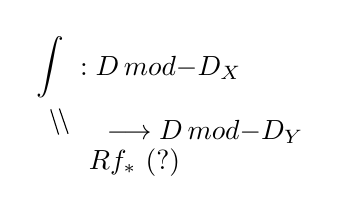
\begin{tikzpicture}[baseline=(int.base)]
\node (int) at (0,0) {$\displaystyle\int$};
\node[anchor=west] at (0.25,0) {$:D\,\text{mod-}D_X$};
\node[anchor=west] at (0.59,-0.82) {$\longrightarrow D\,\text{mod-}D_Y$};
\draw (0,-0.53) -- (0.10,-0.85);
\draw (0.11,-0.52) -- (0.22,-0.84);
\node[anchor=west] at (0.36,-1.20) {$R f_*\ (?)$};
\end{tikzpicture}}\endgroup
\par (12)}
\end{GelfandAdjacentEvidence}
\begin{GelfandAdjacentEvidence}{GELFAND-P000939}{7}


\begin{equation*}
 \int\mathcal M=R f_\bullet
 \left(\mathcal M\mathbin{\underset{D_X}{\overset L\otimes}}\mathcal D_{X\to Y}\right)
 \qquad\text{--- комплекс}
 \tag{13}
\end{equation*}
\Unclear{GELFAND-P000939}{equation-thirteen-cancelled-subscript}{Под $D$ стоит $X$. Рядом зачёркнут прежний знак, который не удаётся прочесть.}
\end{GelfandAdjacentEvidence}
\begin{GelfandAdjacentEvidence}{GELFAND-P000939}{8}

\begin{equation*}
 \int^i\mathcal M=H^i\left(\int\mathcal M\right)
 \tag{14}
\end{equation*}
(Sato, Kashiwara)

(15)\quad \underline{Теорема.} $Y$ --- точка $\Rightarrow$
\begin{equation*}
 \int^i\omega_X=H^{\dim X+i}(X)
 \tag{16}
\end{equation*}
\SourceFigure{GELFAND-P000939}{last-formula-number}{Номер формулы читается (16). Нижняя петля последней цифры замкнута.}
\end{GelfandAdjacentEvidence}
\begin{GelfandAdjacentEvidence}{GELFAND-P000939}{9}

\Incomplete{GELFAND-P000939}{last-exponent-cancellation}{Перед $\dim X+i$ в показателе зачёркнут знак. Точное чтение не установлено.}
\end{GelfandAdjacentEvidence}


($X$ --- неособое над $\mathbb C$)

\Needspace{7\baselineskip}
\begin{GelfandAdjacentEvidence}{GELFAND-P000940}{1}
\SourcePage{GELFAND-P000940}{25}

\underline{С. Гельфанд}

\uwave{Производная категория.}
\SourceFigure{GELFAND-P000940}{derived-title}{В заголовке единственное число «категория».}
\end{GelfandAdjacentEvidence}
\begin{GelfandAdjacentEvidence}{GELFAND-P000940}{2}


\underline{Зад. 1.} Если есть 2 компл. с изом. когомологиями, то не всегда можно изом. когом. прод. до отобр. компл., индуц. изоморфизм.

\underline{Зад. 2.} Рассм. сферу $S^n$ и на ней кат. пучков аб. групп $C$. На ней действ. $O(n)$.
Рассм. кат. с действ. гр. и произв. кат. $D(C)$. Рассм. двойств. $S^{*n}$. $C_1$ [зачёркнуто: не разобрано]
\SourceFigure{GELFAND-P000940}{top-action-abbreviation}{После «действ.» читается сокращение «гр.».}
\end{GelfandAdjacentEvidence}
\begin{GelfandAdjacentEvidence}{GELFAND-P000940}{3}

\Incomplete{GELFAND-P000940}{top-cancelled-symbol}{Знак справа от первого $C_1$ густо зачёркнут.}
\end{GelfandAdjacentEvidence}
\begin{GelfandAdjacentEvidence}{GELFAND-P000940}{4}


$C_1$ не изом. $C$ (действие другое)
\[
 \underline{\underline{D(S)\sim D(S^*)}}\quad!!
\]

\underline{24.11.80 г}\qquad\underline{сем. Гельфанда.}

\uwave{Секционные.}

\underline{25}\quad к. \(\underrightarrow{451}\)\quad [зачёркнуто: не разобрано]
\Unclear{GELFAND-P000940}{section-room-prefix}{Перед 451 стоит сокращение, предположительно «к.».}
\end{GelfandAdjacentEvidence}
\begin{GelfandAdjacentEvidence}{GELFAND-P000940}{5}

\Incomplete{GELFAND-P000940}{section-cancelled-entry}{Зачёркнутая запись перед $15^{00}$ не разобрана.}
\end{GelfandAdjacentEvidence}
\begin{GelfandAdjacentEvidence}{GELFAND-P000940}{6}


\begin{tabular}{@{}ll@{}}
$15^{\underline{00}}$ & Сергеев\\
$15^{\underline{20}}$ & \underline{Mebkhout} (France)\\
& зад. Рим.-Гильб. в высш. размер.\\
$15^{\underline{40}}$ & Хенкин\\
$16^{\underline{00}}$ & \underline{Kantor} J.-M.
\end{tabular}

[рамка справа]

\underline{Конфер.}\qquad\underline{\underline{Пленарные.}}

\begin{tabular}{@{}lll@{}}
\underline{24.} & $16^{\underline{20}}$ & Sato\\
\underline{25} & $10^{\underline{00}}$ & Morimoto\\
 & $10^{\underline{40}}$ & Маслов\\
 & $11^{\underline{40}}$ & Gesztelyi\\
 & & (обобщ. ф-и в ур. частн. (?)\\
 & $12^{\underline{20}}$ & Березанский и др.
\end{tabular}
\Unclear{GELFAND-P000940}{gesztelyi-note-ending}{Окончание строки после «в ур.» читается предположительно как «частн.». Закрывающей скобки не видно.}
\end{GelfandAdjacentEvidence}
\begin{GelfandAdjacentEvidence}{GELFAND-P000940}{7}


\begin{tabular}{@{}lll@{}}
\underline{26.} & [зачёркнуто: не разобрано]\quad\underline{10.00} & \underline{Laugwitz}\\
 & & (с нестанд. т. зрения)\\
 & $10^{\underline{40}}$ & \underline{Иванов}\\
 & $11^{\underline{40}}$ & \underline{Хромов}, \underline{Данилов}\\
 & $12^{\underline{20}}$ & \underline{Berg}\quad умнож. распр.
\end{tabular}
\Incomplete{GELFAND-P000940}{conference-cancelled-time}{Прежнее время перед 10.00 густо зачёркнуто.}
\end{GelfandAdjacentEvidence}
\begin{GelfandAdjacentEvidence}{GELFAND-P000940}{8}


\begin{tabular}{@{}lll@{}}
\underline{28.} & $10^{\underline{00}}$ & \underline{Lions}\\
 & $10^{\underline{40}}$ & \underline{Гельфанд}\\
 & $11^{\underline{40}}$ & \underline{Komatsu} --- ядра в ультрараспред.\\
 & $12^{\underline{20}}$ & \underline{Lassner}\\
 & $13^{\underline{00}}$ & \underline{Жаринов}
\end{tabular}

\underline{Д. Б. Фукс.}\qquad\underline{Умн. Уайтхеда}
\[
 \pi_n(X)\times\pi_m(X)\longrightarrow\pi_{n+m}(X)
\]
$\sim$ коммутатор в алг. Ли
\[
 \partial(I_n\times I_m)=(\partial I_n\times I_m)\cup(I_n\times\partial I_m)
\]
Тождество Якоби есть --- суперсим. Ли!!
\SourceFigure{GELFAND-P000940}{fuchs-final-abbreviation}{Перед «Ли» читается сокращение «суперсим.».}
\end{GelfandAdjacentEvidence}
\begin{GelfandAdjacentEvidence}{GELFAND-P000940}{9}


\underline{\underline{В. Ломоносов.}}

$(A-A')$ --- ядерный

$B$ комм. с $A$, $B$ комм. с $A'$, $(B-B')$ --- вп. непр
\SourceFigure{GELFAND-P000940}{lomonosov-second-B}{Перед $A'$ написано $B$ без видимого штриха.}
\end{GelfandAdjacentEvidence}
\begin{GelfandAdjacentEvidence}{GELFAND-P000940}{10}

\[
 \Rightarrow\quad B|_{\mathcal H_{ac}(B)}\underset{\text{унит.}}{\sim}
 B'|_{\mathcal H_{ac}(B')}
\]
$\Rightarrow$ теор. расс. сразу для коммут. сем-в операторов.

\underline{\underline{А. Бейлинсон.}}

\(X\overset f\longrightarrow Y\)
\begin{equation*}
 f^*:\mathcal D_Y\text{-mod}\longrightarrow\mathcal D_X\text{-mod}
 \tag{1}
\end{equation*}
Введём
\[
 f_*:\text{mod-}\mathcal D_X\longrightarrow\text{mod-}\mathcal D_Y
\]
[справа]
\[
 \left[\begin{aligned}
 &\text{если }\overset{\text{на $Y$}}{u}\text{ уд. сист. }M,\\
 &\text{то }f^*u\text{ уд. сист. }f^*M
 \end{aligned}\right.
\]
\SourceFigure{GELFAND-P000940}{upper-bracketed-note}{«на $Y$» вписано над $u$ в верхней записи справа.}
\end{GelfandAdjacentEvidence}
\begin{GelfandAdjacentEvidence}{GELFAND-P000940}{11}


\begin{equation*}
 \mathcal D_{X\to Y}=f^*(\mathcal D_Y)\in\mathcal D_X\text{-mod-}\mathcal D_Y
 \qquad\text{(бимодуль)}
 \tag{2}
\end{equation*}
\begin{equation*}
 f_*M=f_\bullet\left(M\mathbin{\underset{\mathcal D_X}{\otimes}}\mathcal D_{X\to Y}\right)
 \tag{3}
\end{equation*}
(\(\underset{\text{если}}{f_*}\) на формах объёма с комп. носителем)

[справа]
\[
 \left[\begin{aligned}
 &\text{если }u\ \overset{\in\Omega_1(X)}{\text{на $X$}}\text{ уд. сист. }M,\\
 &\text{то }f_*u\text{ уд. сист. }f_*M
 \end{aligned}\right.
\]
\Unclear{GELFAND-P000940}{lower-right-omega-insertion}{Малый индекс у $\Omega$ похож на $1$. Точное чтение не установлено.}
\end{GelfandAdjacentEvidence}
\begin{GelfandAdjacentEvidence}{GELFAND-P000940}{12}

\SourceFigure{GELFAND-P000940}{lower-bracketed-note}{Нижняя запись справа начинается с открытой квадратной скобки.}
\end{GelfandAdjacentEvidence}


\Needspace{7\baselineskip}
\begin{GelfandAdjacentEvidence}{GELFAND-P000941}{1}
\SourcePage{GELFAND-P000941}{unlabelled}

(Сист. ур-й, к-рой удовл. несобственные интегралы)

(4)\quad $f_*$ не функториально: \qquad $(fg)_*\ne f_*g_*$
\SourceFigure{GELFAND-P000941}{ordinary-composition}{В (4) $fg$ и $f_*g_*$ записаны в таком порядке.}
\end{GelfandAdjacentEvidence}
\begin{GelfandAdjacentEvidence}{GELFAND-P000941}{2}


Строим.
\begin{equation*}
 Rf_*:D(\text{mod-}D_X)\longrightarrow D(\text{mod-}D_Y)
 \tag{5}
\end{equation*}

\underline{Пример:} $X$ --- плоскость, $Y$ --- прямая, $f$ --- проекция,

$\mathcal M$ --- пучок форм на $X$ (старшей степени)
\[
 Rf_*(\mathcal M)\text{ --- комплекс,}\qquad
 \begin{aligned}
 &0\text{-комп. --- }0\\
 &(-1)\text{-комп. --- }\text{\uwave{формы на прямой.}}
 \end{aligned}
\]
\SourceFigure{GELFAND-P000941}{example-components}{В примере записаны $0$-комп. и $(-1)$-комп.}
\end{GelfandAdjacentEvidence}
\begin{GelfandAdjacentEvidence}{GELFAND-P000941}{3}


\begin{equation*}
 Rf_*(\mathcal M)=Rf_\bullet
 \left(\mathcal M\mathbin{\underset{\mathcal D_X}{\overset L\otimes}}\mathcal D_{X\to Y}\right)
 \tag{6}
\end{equation*}
$\overset L\otimes$ --- левый произв. функтор от тенз. произвед.

$Rf_\bullet$ --- правый произв. функтор от функтора (!) $f_\bullet$

(7)\quad \underline{Предл.}
\SourceFigure{GELFAND-P000941}{derived-composition}{Под цепочкой $X\to Y\to Z$ двойная стрелка вниз к формуле.%
\par\smallskip
\begingroup\color{black}\GelfandFitDiagram{\begin{tikzpicture}[baseline=(maps.base)]
\node (maps) at (0,0) {$X\overset f\longrightarrow Y\overset g\longrightarrow Z$};
\node at (0,-0.63) {$\Downarrow$};
\node at (0,-1.23) {$Rg_*Rf_*=R(g\circ f)_*$};
\end{tikzpicture}}\endgroup}
\end{GelfandAdjacentEvidence}
\begin{GelfandAdjacentEvidence}{GELFAND-P000941}{4}


[зачёркнуто: \sout{(так}] ($f_*$ не облад. этим св-вом)
\Unclear{GELFAND-P000941}{cancelled-word-before-parenthesis}{Перед открывающей скобкой зачёркнуто начало «(так».}
\end{GelfandAdjacentEvidence}
\begin{GelfandAdjacentEvidence}{GELFAND-P000941}{5}


Пусть
\[
 \mathcal M\in\text{mod-}\mathcal D_X
\]
\begin{equation*}
 \ldots\longrightarrow\mathcal M\otimes\Lambda^2T_X
 \longrightarrow\mathcal M\otimes T_X\underset{\nearrow}{\longrightarrow}\mathcal M
 \tag{8}
\end{equation*}
($T_X$ --- касат. пучок к $X$)\qquad (т.к. $\mathcal M$ --- правый
 $\mathcal D_X\text{-mod},\ T_X\subset\mathcal D_X$)
\SourceFigure{GELFAND-P000941}{last-differential-leader}{От правого примечания стрелка идёт к последнему дифференциалу (8).}
\end{GelfandAdjacentEvidence}
\begin{GelfandAdjacentEvidence}{GELFAND-P000941}{6}


(9)\quad \underline{Предл.}

\uwave{Рассм. когомологии} (8). \uwave{Они совпад. с когом. компл.} (6), т.е.

\hspace{2em}(де Рама!)
\begin{equation*}
 R\Gamma(\underbrace{DR}_{\text{De Rham}}\mathcal M)=Rf_*(\mathcal M)
 \tag{10}
\end{equation*}
(\uwave{здесь} $f:X\longrightarrow\text{\uwave{точка}}$).
\SourceFigure{GELFAND-P000941}{de-rham-underlabel}{Под $DR$ имеется скобка с подписью «De Rham».}
\end{GelfandAdjacentEvidence}
\begin{GelfandAdjacentEvidence}{GELFAND-P000941}{7}


$\mathcal M$ --- пучок форм объёма $\Rightarrow$ (8) --- обычный компл. де Рама, но сдвинутый на $\mathcal M$ влево
\Unclear{GELFAND-P000941}{de-rham-shift-amount}{После «на» стоит знак, похожий на $\mathcal M$ в начале фразы.}
\end{GelfandAdjacentEvidence}
\begin{GelfandAdjacentEvidence}{GELFAND-P000941}{8}


\SourceFigure{GELFAND-P000941}{volume-omega-leader}{От пометы к $\omega$ идёт наклонная черта.%
\par\smallskip
\begingroup\color{black}\GelfandFitDiagram{\begin{tikzpicture}[baseline=(omega.base)]
\node (omega) at (0,0) {$\omega$};
\node[anchor=east] at (-0.16,0) {$R^if_*$};
\node[anchor=west] at (0.15,0) {$=H^{\dim X+i}(X)$};
\node[anchor=west] at (0.26,0.66) {\scriptsize пучок всех форм объёма};
\draw (0.05,0.21) -- (0.33,0.51);
\end{tikzpicture}}\endgroup
\par (11)}
\end{GelfandAdjacentEvidence}
\begin{GelfandAdjacentEvidence}{GELFAND-P000941}{9}


Более общ.: \uwave{Для гладкого морфизма --- пучки когом. вдоль слоёв!}
\begin{equation*}
 \ldots\longrightarrow\mathcal M\otimes\Lambda^2T_{X/Y}
 \longrightarrow\mathcal M\otimes T_{X/Y}\longrightarrow\mathcal M
 \quad\leftarrow\quad(\text{это }DR_{X/Y}\mathcal M)
 \tag{12}
\end{equation*}
\SourceFigure{GELFAND-P000941}{relative-de-rham}{Короткая стрелка направлена влево от пометы в скобках к комплексу.}
\end{GelfandAdjacentEvidence}


\Needspace{7\baselineskip}
\begin{GelfandAdjacentEvidence}{GELFAND-P000942}{1}
\SourcePage{GELFAND-P000942}{26}

Тогда
\begin{equation*}
 Rf_\bullet(DR_{X/Y}\mathcal M)=Rf_*(\mathcal M)
 \tag{13}
\end{equation*}

Итак, в прямом образе [вписано сверху: относит.] DeRhama ввод. \underline{действие дифф. операторов} (!)
\SourceFigure{GELFAND-P000942}{relative-dr-complex-word}{В строке читается «DeRhama». Над началом этой записи вставлено «относит.».}
\end{GelfandAdjacentEvidence}
\begin{GelfandAdjacentEvidence}{GELFAND-P000942}{2}


(не очевидно, т.к. в исх. пучке [зачёркнуто: \sout{его} (?)] [вписано сверху: не разобрано] нет). Это действие назыв.
\Unclear{GELFAND-P000942}{overwritten-word-before-net}{Перед «нет» нижнее слово сильно обведено, предположительно «его». Над ним короткая неразобранная вставка.}
\end{GelfandAdjacentEvidence}
\begin{GelfandAdjacentEvidence}{GELFAND-P000942}{3}


\uwave{связностью Гаусса-Манина.}

\underline{2-й случай}

$X\overset f\longrightarrow Y$\qquad\uwave{вложение.}
\begin{equation*}
 \begin{aligned}
 Rf_*(\mathcal M)&=Rf_\bullet
 \left(\mathcal M\mathbin{\underset{\mathcal D_X}{\overset L\otimes}}\mathcal D_{X\to Y}\right)\\
 &=f_\bullet
 \left(\mathcal M\mathbin{\underset{\mathcal D_X}{\overset L\otimes}}\mathcal D_{X\to Y}\right)=
 \end{aligned}
 \tag{14}
\end{equation*}
\SourceFigure{GELFAND-P000942}{embedding-equality}{На конце первой строки (14) после второго выражения стоит ещё один знак равенства.}
\end{GelfandAdjacentEvidence}
\begin{GelfandAdjacentEvidence}{GELFAND-P000942}{4}


(Функтор $f_\bullet$ в этом случае точен ---)

--- не возник. когом. вдоль слоёв
\[
 =f_\bullet\left(\mathcal M\mathbin{\underset{\mathcal D_X}{\otimes}}\mathcal D_{X\to Y}\right)
\]
(т.к. $\otimes$ в этом случае точен)

$\omega\rightsquigarrow$ формы, прод. $\delta$-ф-ями в трансверс. направл.

\underline{Голономные модули.}

$X$ --- мн-зие, $\mathcal M$ --- конечно порожд.
\(\overset{\mathcal D_X\text{-}}{\text{модуль}}\) [зачёркнуто: не разобрано]
\SourceFigure{GELFAND-P000942}{module-insertion}{Перед словом «модуль» сверху вписано $\mathcal D_X$-.}
\end{GelfandAdjacentEvidence}
\begin{GelfandAdjacentEvidence}{GELFAND-P000942}{5}

\Incomplete{GELFAND-P000942}{cancelled-module-end}{Конец строки после «модуль» зачёркнут. Похож на $\mathcal M$, но чтение не установлено.}
\end{GelfandAdjacentEvidence}
\begin{GelfandAdjacentEvidence}{GELFAND-P000942}{6}


Он наз. \uwave{голономным}, если $\forall\,x\in X$,
\[
 \text{\uwave{когомологии}}\quad Li_x^*\mathcal M\quad
 \text{\uwave{конечномерны}}
\]
(слой модуля над точкой)
\SourceFigure{GELFAND-P000942}{point-inclusion-diagram}{Стрелка $i_x$ ведёт от $x$ к $X$. Перед $x$ есть неразобранный густой штрих.%
\par\smallskip
\begingroup\color{black}\GelfandFitDiagram{\begin{tikzpicture}[baseline=(x.base)]
\node (x) at (0,0) {$( [\text{?}]\,x$};
\node (X) at (2.35,0) {$X )$};
\draw[->] (x.east) to[out=15,in=173] node[above] {$i_x$} (X.west);
\node at (1.28,-0.55) {\scriptsize вложение};
\end{tikzpicture}}\endgroup}
\end{GelfandAdjacentEvidence}
\begin{GelfandAdjacentEvidence}{GELFAND-P000942}{7}


($i_x^*\mathcal M$ --- «замораживание коэфф.» --- см. выше)

$\sim$ комплекс $Li_x^*\mathcal M$ конечномерен (т.к. в произв. категории).

\uwave{Своб. модуль}\quad\uwave{не явл. голономным} (см. прошл. раз)

Голономность $\sim$ переопределённость.

\underline{Примеры}

а)\enspace [вписано сверху: $X=\mathbb R^1$ (?)] рассл. с интегр. связностью
\SourceFigure{GELFAND-P000942}{example-a-field}{Буква поля обведена и имеет нижний косой штрих. Предположительное чтение $\mathbb R^1$.}
\end{GelfandAdjacentEvidence}
\begin{GelfandAdjacentEvidence}{GELFAND-P000942}{8}


Модуль так устроен, кроме конечн. числа точек, где могут быть особ.

б)\enspace $X=\mathbb C^2$ опять на доп. к конечн. числу [зачёркнуто: \sout{точек} (?)]
[вписано сверху: кривых] --- рассл. с интегр. связн.
\SourceFigure{GELFAND-P000942}{example-b-cancelled-word}{Под вписанным «кривых» зачёркнуто прежнее слово. Возможно, «точек».}
\end{GelfandAdjacentEvidence}
\begin{GelfandAdjacentEvidence}{GELFAND-P000942}{9}


На этих кривых --- особенности.

\tikz[baseline=(q.base)]{\node[draw,circle,inner sep=2pt] (q) {?};}
\uwave{Все получ. склейкой} из модулей, получ. из $\delta$-ф-й по нормали.
\SourceFigure{GELFAND-P000942}{circled-question}{Слева от строки о склейке обведён вопросительный знак.}
\end{GelfandAdjacentEvidence}
\begin{GelfandAdjacentEvidence}{GELFAND-P000942}{10}


[зачёркнуто: \sout{(кроме точек […] кривых} не разобрано]
\Unclear{GELFAND-P000942}{last-cancelled-middle}{В середине зачёркнутой строки читается предположительно «точек». Следующее слово не установлено.}
\end{GelfandAdjacentEvidence}
\begin{GelfandAdjacentEvidence}{GELFAND-P000942}{11}

\Incomplete{GELFAND-P000942}{last-cancelled-tail}{После «кривых» видна ещё зачёркнутая запись. Окончание не установлено.}
\end{GelfandAdjacentEvidence}


\Needspace{7\baselineskip}
\begin{GelfandAdjacentEvidence}{GELFAND-P000943}{1}
\SourcePage{GELFAND-P000943}{unlabelled}

(15)\quad\underline{Теор.}\enspace 1) $\forall$ \uwave{голон. модуль имеет конечную длину}

(фильтрации с непр. факторами им. од. длину)
\Unclear{GELFAND-P000943}{filtration-length}{Окончание первого слова в скобках слабо различимо. Последняя строка читается «им. од. длину».}
\end{GelfandAdjacentEvidence}
\begin{GelfandAdjacentEvidence}{GELFAND-P000943}{2}


2)\enspace \uwave{есть опис. всех неприводимых}
\[
 Y\subset X,\qquad Y\text{ непривод.}
\]

Непривод. [вписано сверху и обведено: плоское] рассл. $\mathcal L_Y$ со связностью на $Y$

(векторное рассл. с интегр. св.)
\SourceFigure{GELFAND-P000943}{flat-insertion}{К слову «рассл.» идёт выноска от обведённого «плоское».%
\par\smallskip
\begingroup\color{black}\GelfandFitDiagram{\begin{tikzpicture}[baseline=(b.base)]
\node (b) at (0,0) {\small Непривод.\quad рассл.};
\node (f) at (0.12,0.58) {\scriptsize плоское};
\draw (f) ellipse (0.63 and 0.24);
\draw (-0.20,0.39) to[out=-24,in=104] (0.02,0.05);
\draw (0.02,0.05) to[out=76,in=-153] (0.44,0.39);
\end{tikzpicture}}\endgroup}
\end{GelfandAdjacentEvidence}
\begin{GelfandAdjacentEvidence}{GELFAND-P000943}{3}


2 пары $Y_1,Y_2$ наз. эквив., если $Y_1$ открыто в $Y_2$

и
\[
 \mathcal L_{Y_1}=\left.\left(\mathcal L_{Y_2}\right)\right|_{Y_1}
\]
\SourceFigure{GELFAND-P000943}{generic-point}{Условие в строке дано в порядке «$Y_1$ открыто в $Y_2$».}
\end{GelfandAdjacentEvidence}
\begin{GelfandAdjacentEvidence}{GELFAND-P000943}{4}


(можно выброс. замкн. подмн-ва, зад. над общей точкой)

(16)\quad\underline{\underline{Утв.}}\quad $i:Y\hookrightarrow X$

\uwave{В \(i_*\mathcal L_Y\) есть единств. неприв. подмодуль} ---
\SourceFigure{GELFAND-P000943}{unique-submodule}{В рукописи под строкой две волнистые линии разной длины.}
\end{GelfandAdjacentEvidence}
\begin{GelfandAdjacentEvidence}{GELFAND-P000943}{5}


это и есть искомый объект --- непривод. модуль

$Y$ --- гладкое $\Rightarrow$ уже неприводимо

В особ. появл. $\delta$-ф-и.
\SourceFigure{GELFAND-P000943}{terminal-vignette}{Под последней строкой две клиновидные черты с точкой между ними.%
\par\smallskip
\begingroup\color{black}\GelfandFitDiagram{
\begin{tikzpicture}
\fill (-1.48,-0.05) -- (-0.31,0.14) -- (-0.31,-0.08) -- cycle;
\fill (0.02,-0.02) circle (0.11);
\fill (0.36,0.13) -- (1.54,0.05) -- (0.36,-0.08) -- cycle;
\end{tikzpicture}}\endgroup}
\end{GelfandAdjacentEvidence}


\Needspace{7\baselineskip}
\begin{GelfandAdjacentEvidence}{GELFAND-P000944}{1}
\SourcePage{GELFAND-P000944}{27}

$1/\underline{\overline{\mathrm{XII}}}$-80 г.\qquad \underline{Сем. Гельфанда.}
\SourceFigure{GELFAND-P000944}{hatched-date}{Дата подчёркнута узкой полосой с поперечными штрихами. Над и под XII отдельные черты.%
\par\smallskip
\begingroup\color{black}\GelfandFitDiagram{\begin{tikzpicture}[baseline=(date.base)]
\node[anchor=west,inner sep=0pt] (date) at (0,0) {$1/\underline{\overline{\mathrm{XII}}}$-80 г.};
\draw (0,-0.23) -- (2.45,-0.26) -- (2.39,-0.38) -- (0.02,-0.35) -- cycle;
\foreach \x in {0.31,0.59,0.88,1.17,1.46,1.75,2.04,2.30}
 {\draw (\x,-0.25) -- ++(-0.04,-0.11);}
\end{tikzpicture}}\endgroup}
\end{GelfandAdjacentEvidence}
\begin{GelfandAdjacentEvidence}{GELFAND-P000944}{2}


\underline{С. П. Новиков.}

\begin{equation*}
 \hat H=\frac12\sum_{\alpha=1}^n
 \left(i\frac{\partial}{\partial x^\alpha}-eA_\alpha\right)^2
 +cV(\vec x)
 \tag{1}
\end{equation*}
\Incomplete{GELFAND-P000944}{equation-one-cancellation}{После знака равенства в (1), перед дробью, есть густо зачёркнутая запись. Она не разобрана.}
\end{GelfandAdjacentEvidence}
\begin{GelfandAdjacentEvidence}{GELFAND-P000944}{3}


\begin{equation*}
 H_{\alpha\beta}=\partial_\beta A_\alpha-\partial_\alpha A_\beta
 \tag{2}
\end{equation*}
$V$ --- эл. поле, $H_{\alpha\beta}$ --- магн. поле

\begin{equation*}
 \hat H\psi=\varepsilon\psi\qquad\text{спектр. задача.}
 \tag{3}
\end{equation*}

Интересен случай, когда

(4)\quad $H_{\alpha\beta}(x)$ и $V(x)$ период. с решёткой периодов.
\SourceFigure{GELFAND-P000944}{lattice-cell}{Ячейка $K_{12}$ между стрелками $T_1,T_2$. Верхняя и правая стороны прерывистые.%
\par\smallskip
\begingroup\color{black}\GelfandFitDiagram{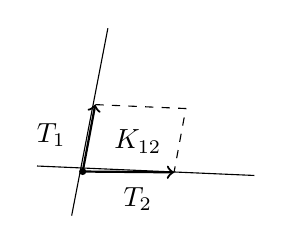
\begin{tikzpicture}
\draw (-0.58,0.07) -- (2.18,-0.05);
\draw (-0.14,-0.56) -- (0.32,1.82);
\draw[thick,->] (0,0) -- (0.16,0.85);
\draw[thick,->] (0,0) -- (1.16,-0.01);
\draw[dashed] (0.16,0.85) -- (1.31,0.80) -- (1.16,-0.01);
\fill (0,0) circle (0.045);
\node at (-0.40,0.46) {$T_1$};
\node at (0.70,-0.35) {$T_2$};
\node at (0.70,0.38) {$K_{12}$};
\end{tikzpicture}}\endgroup}
\end{GelfandAdjacentEvidence}
\begin{GelfandAdjacentEvidence}{GELFAND-P000944}{4}


(не только эл. поле, но и его потенциал; постоянное эл. поле --- неразумно)
\Unclear{GELFAND-P000944}{constant-electric-word}{Слово после тире предположительно читается «неразумно». Конец бледный.}
\end{GelfandAdjacentEvidence}
\begin{GelfandAdjacentEvidence}{GELFAND-P000944}{5}


--- потенциал тогда $\vec E\cdot\vec x$ [зачёркнуто: не разобрано] ---
\Incomplete{GELFAND-P000944}{electric-potential-cancellation}{После $\vec E\cdot\vec x$ зачёркнут один знак. Точное чтение не установлено.}
\end{GelfandAdjacentEvidence}
\begin{GelfandAdjacentEvidence}{GELFAND-P000944}{6}


\uwave{--- не изучена даже 1-мерн. задача.})

$A_\alpha$ не периодичен (вообще говоря).

$K_{\alpha\beta}$ --- ячейка (элем.), нат. на $\alpha$ и $\beta$ координату
\Unclear{GELFAND-P000944}{cell-preposition}{Предлог после «нат.» переписан и предположительно читается «на».}
\end{GelfandAdjacentEvidence}
\begin{GelfandAdjacentEvidence}{GELFAND-P000944}{7}

\Unclear{GELFAND-P000944}{cell-coordinate-ending}{Конец слова «координату» переписан. Последняя буква читается «у».}
\end{GelfandAdjacentEvidence}
\begin{GelfandAdjacentEvidence}{GELFAND-P000944}{8}


\begin{equation*}
 \iint_{K_{\alpha\beta}}H_{\alpha\beta}\,dx^\alpha\wedge dx^\beta
 =\Phi_{\alpha\beta}\qquad\text{--- магн. потоки (базисные)}
 \tag{5}
\end{equation*}
(суммир. нет!)

\begin{equation*}
 i\nabla_\alpha=i\frac{\partial}{\partial x^\alpha}-eA_\alpha
 \qquad\text{имеет смысл связности}
 \tag{6}
\end{equation*}

\underline{Замеч.} Спин здесь $0$, со спином $1/2$ будет
\begin{equation*}
 \hat H=(1)+e\sigma_jH^j,\qquad\text{где }
 H^1=H_{23},\quad H^2=-H_{13},\quad H^3=H_{12};
 \tag{7}
\end{equation*}
$\sigma_1,\sigma_2,\sigma_3$ --- матр. Паули

(8)\quad\uwave{Допустимый случай:} \(\dfrac e{2\pi}\Phi_{\alpha\beta}\in\mathbb Z\)

Оператор $\hat H$ рассм. в $L^2(\mathbb R^n)$.

(9)\quad $(8)\Rightarrow\hat H$ --- универс. накрыв. опер. на торе (в расслоении), причём
\Unclear{GELFAND-P000944}{covering-overwritten-word}{Начало слова «причём» обведено.}
\end{GelfandAdjacentEvidence}
\begin{GelfandAdjacentEvidence}{GELFAND-P000944}{9}


\begin{equation*}
 \left(c_1(\xi),\underset{\substack{\vert\\\text{баз. цикл}}}{Z_{\alpha\beta}}\right)
 =\frac e{2\pi}\Phi_{\alpha\beta}
 \tag{10}
\end{equation*}
\SourceFigure{GELFAND-P000944}{chern-cycle}{Под $Z_{\alpha\beta}$ короткий штрих к подписи «баз. цикл».}
\end{GelfandAdjacentEvidence}
\begin{GelfandAdjacentEvidence}{GELFAND-P000944}{10}


Однако опер. всегда имеет смысл (физич.), но теории нет.

(11)\quad Иррацион. интер. \uwave{Рац. свод. к нему укрупнением решётки}
\Unclear{GELFAND-P000944}{irrational-final-abbreviation}{Сокращение после «Иррацион.» предположительно читается «интер.».}
\end{GelfandAdjacentEvidence}


\Needspace{7\baselineskip}
\begin{GelfandAdjacentEvidence}{GELFAND-P000945}{1}
\SourcePage{GELFAND-P000945}{unlabelled}

\dashuline{Магнитные трансляции.}
\SourceFigure{GELFAND-P000945}{broken-underline}{Под заголовком прерывистая черта.}
\end{GelfandAdjacentEvidence}
\begin{GelfandAdjacentEvidence}{GELFAND-P000945}{2}


\underline{2 типа задач:} а) [зачёркнуто: \sout{магн.} (?)] реш. навязана (тв. тел!), а магн. поле извне
\Unclear{GELFAND-P000945}{top-cancelled-abbreviation}{Перед «реш.» зачёркнутое сокращение предположительно читается «магн.».}
\end{GelfandAdjacentEvidence}
\begin{GelfandAdjacentEvidence}{GELFAND-P000945}{3}


б)\enspace типа сверхпров.: магн. поле само возникает, они автоматич. целочисл.

а)\enspace $K_{\alpha\beta}\sim10^{-10}\text{ см}^2$
\qquad б)\enspace $\sim10^{-16}\text{ см}^2$
\SourceFigure{GELFAND-P000945}{cell-areas}{В строке записаны $10^{-10}$ и $10^{-16}$ в квадратных сантиметрах.}
\end{GelfandAdjacentEvidence}
\begin{GelfandAdjacentEvidence}{GELFAND-P000945}{4}


\underline{Магн. трансл.}\qquad Имеем:
\begin{equation*}
 A_\alpha(\ldots,x^i+T_i,\ldots)=A_\alpha(x)+\partial_\alpha f_i
 \tag{12}
\end{equation*}
(т.к. $dA$ периодичен)

\begin{equation*}
 \hat T_j^*\psi(x)=\psi(\mathinner{..}\,x^{j}+T_j,\,)\exp(-ie f_j)
 \tag{13}
\end{equation*}
(опер. магн. трансляции)
\Unclear{GELFAND-P000945}{translation-coordinate-superscript}{В (13) верхний индекс у $x$ обведён. Чтение $j$ предположительно и согласуется с $T_j$ в той же строке.}
\end{GelfandAdjacentEvidence}
\begin{GelfandAdjacentEvidence}{GELFAND-P000945}{5}


(14)\quad\underline{Лемма 1} (известная $\sim$60-е годы
[зачёркнуто: не разобрано], \uwave{Зак и Браун})
\begin{equation*}
 \hat T_j^*\hat T_k^*=\hat T_k^*T_j^*\exp(-ie\Phi_{kj}),
 \qquad j,k=1,\ldots,n.
\end{equation*}
\Unclear{GELFAND-P000945}{lemma-cancelled-character}{После «годы» густо переписан знак. Точное чтение не установлено.}
\end{GelfandAdjacentEvidence}
\begin{GelfandAdjacentEvidence}{GELFAND-P000945}{6}

\SourceFigure{GELFAND-P000945}{commutator-hats}{У последнего $T_j^*$ справа в равенстве шляпки не видно.}
\end{GelfandAdjacentEvidence}
\begin{GelfandAdjacentEvidence}{GELFAND-P000945}{7}


Получилось проективное предст. аб. группы, коциклы заранее заданы.

Иррац. потоки $\Rightarrow$ получ. группы не типа 1. (подгр. в гр. Гейзенберга).

\begin{equation*}
 \frac{e\Phi_{kj}}{2\pi}\in\mathbb Z\Rightarrow\text{коммут. группа}
 \tag{15}
\end{equation*}
$\underline{n=2}$

($n=3$ тоже интересно)

сверхпров. --- 2-мерн. задача

\underline{Задача:} описать спектр $\hat H$.

(16)\quad $[\hat H,\hat T_j^*]=0\Rightarrow$ соб. ф-и надо искать одновр. собств. для $\hat T_j^*$

[зачёркнуто под строкой: \sout{магн.} (?)]
\Unclear{GELFAND-P000945}{eigenfunction-cancelled-abbreviation}{Под строкой (16) зачёркнуто сокращение, похожее на «магн.».}
\end{GelfandAdjacentEvidence}
\begin{GelfandAdjacentEvidence}{GELFAND-P000945}{8}


Магнито-блоховские:
\begin{equation*}
 \hat T_j^*\psi_{p}=\exp(ip_jT_j)\psi_{p}
 \tag{17}
\end{equation*}
\Unclear{GELFAND-P000945}{bloch-subscript-left}{Индекс у левой $\psi$ густо переписан. $p$ восстановлено предположительно по соседней строке.}
\end{GelfandAdjacentEvidence}
\begin{GelfandAdjacentEvidence}{GELFAND-P000945}{9}

\Unclear{GELFAND-P000945}{bloch-subscript-right}{Индекс у правой $\psi$ тоже густо переписан. $p$ восстановлено предположительно.}
\end{GelfandAdjacentEvidence}
\begin{GelfandAdjacentEvidence}{GELFAND-P000945}{10}


Опер. в $L^2$ $=$ прямой инт. опер. на торе с такими гран. усл.

$p_j$ --- \uwave{квазиимпульсы}\qquad $(p_1,p_2)\in\mathbb T^2$
\qquad (тор обр. решётки)

Фиксируем $p_1,p_2\Rightarrow$ опер. в рассл. на торе с соб. знач.
\SourceFigure{GELFAND-P000945}{fixed-eigenvalues}{Последние два сокращения читаются «соб. знач.».}
\end{GelfandAdjacentEvidence}


\begin{equation*}
 \varepsilon_j(p_1,p_2)\qquad\text{--- закон дисперсии}
 \tag{18}
\end{equation*}
\[
 j=1,2,\ldots
\]

\Needspace{7\baselineskip}
\begin{GelfandAdjacentEvidence}{GELFAND-P000946}{1}
\SourcePage{GELFAND-P000946}{28}

(19) \underline{Теорема}. \underline{Пусть} $V=0$, \underline{спин} $s=\frac12$,
\[
 n=2,\qquad N\underset{\mathrm{def}}{=}\frac{e\Phi_{12}}{2\pi}.
\]

[На правом поле, за двойной чертой]\par
Дубровин, Новиков\par
ЖЭТФ, сент. 1980.\par
и ещё есть раб. в ДАН
\SourceFigure{GELFAND-P000946}{marginal-citation}{Ссылки на правом поле.}
\end{GelfandAdjacentEvidence}
\begin{GelfandAdjacentEvidence}{GELFAND-P000946}{2}


(магн. поле напр. по оси $Z$ --- 2-мерн. случай --- и период.)

\underline{Тогда} \underline{задав} $A=(a_1,\ldots,a_N)\in C^N$, \underline{мы} \underline{получим}, \underline{что} \underline{соб.} ф-я \underline{им. вид}
[над «соб.» вписано $(\forall\ \text{магн.-блох.})$]
\SourceFigure{GELFAND-P000946}{bloch-insertion}{Надстрочная вставка связана с основной строкой фигурной чертой.}
\end{GelfandAdjacentEvidence}
\begin{GelfandAdjacentEvidence}{GELFAND-P000946}{3}


\begin{equation*}
 \Psi_A=\exp(-e\varphi)\prod_{j=1}^N\sigma(z-a_j)\exp(-az).
 \tag{20}
\end{equation*}
\SourceFigure{GELFAND-P000946}{sigma-exp-sign}{В (20) перед $az$ стоит минус.}
\end{GelfandAdjacentEvidence}
\begin{GelfandAdjacentEvidence}{GELFAND-P000946}{4}

($\sigma$ --- элл. ф-я Вейерштрасса)\par
одна из $\theta$-ф-й
\SourceFigure{GELFAND-P000946}{sigma-note}{Помета справа к (20).}
\end{GelfandAdjacentEvidence}
\begin{GelfandAdjacentEvidence}{GELFAND-P000946}{5}


\begin{equation*}
 p=p_1+ip_2=\frac{2\pi i}{T_1T_2}\sum a_j+
 \underset{\substack{\vert\\\text{зав. от магн. поля}}}{\operatorname{const}(H)},
 \tag{21}
\end{equation*}
\SourceFigure{GELFAND-P000946}{quasimomentum-sign}{Слагаемое с суммой в (21) записано со знаком плюс.}
\end{GelfandAdjacentEvidence}
\begin{GelfandAdjacentEvidence}{GELFAND-P000946}{6}

\SourceFigure{GELFAND-P000946}{field-constant}{Помета под $\operatorname{const}(H)$ связана с ним чертой.}
\end{GelfandAdjacentEvidence}
\begin{GelfandAdjacentEvidence}{GELFAND-P000946}{7}

\[
 \mathcal D=\sum a_j.\qquad\text{(дивизор)}
\]

(22) [зачёркнуто: \sout{\(\varphi(x,y)\)} (?)]
\begin{equation*}
 \varphi(x,y)=\frac{1}{2\pi}\int_{K_{12}}\ln|\sigma(z-z')|H(z')\,d^2z'.
\end{equation*}
\Unclear{GELFAND-P000946}{eq22-cancel}{Перед формулой (22) предположительно зачёркнуто $\varphi(x,y)$.}
\end{GelfandAdjacentEvidence}
\begin{GelfandAdjacentEvidence}{GELFAND-P000946}{8}

\(z={}\)[зачёркнуто: запись не разобрана] \(x+iy\).
\Incomplete{GELFAND-P000946}{z-cancel}{После знака равенства зачёркнуто несколько знаков. Точное чтение не установлено.}
\end{GelfandAdjacentEvidence}
\begin{GelfandAdjacentEvidence}{GELFAND-P000946}{9}


Ф-и (20) --- полный базис решений ур-я $\hat H\psi=0$

(точная интегр. на нижнем нулевом ур. энергии)
\SourceFigure{GELFAND-P000946}{exact-abbr}{Сокращение после «точная» читается «интегр.».}
\end{GelfandAdjacentEvidence}
\begin{GelfandAdjacentEvidence}{GELFAND-P000946}{10}


[зачёркнуто: $L^2=(L^2)^0+\ldots$ (?)]
\Incomplete{GELFAND-P000946}{l2-cancel}{Начало зачёркнутой формулы читается предположительно. Окончание после плюса не разобрано.}
\end{GelfandAdjacentEvidence}
\begin{GelfandAdjacentEvidence}{GELFAND-P000946}{11}

\[
 L_2=L_2+L_2^\perp.
\]
\SourceFigure{GELFAND-P000946}{l2-split}{Петля над первым $L_2$ справа продолжается в выносной штрих строки выше.}
\end{GelfandAdjacentEvidence}
\begin{GelfandAdjacentEvidence}{GELFAND-P000946}{12}


\begin{equation*}
 a=a(a_1,\ldots,a_N)\quad\text{--- \underline{вычисляется}}.
 \tag{23}
\end{equation*}

Выделение завис. (23) --- это выдел. вещ. \underline{квазиимпульсов}

(ф-я $\Psi_A$ всегда собств. и блоховская).

$\lambda\Psi_A$ тоже соб. ф-я

$(\lambda,a_1,\ldots,a_N)$ --- полное мн-во параметров.

\underline{Замеч.}
\begin{equation*}
 (\lambda,a_1,\ldots,a_N)\overset{P}{\longrightarrow}\mathbb T^2.
 \tag{24}
\end{equation*}

(25) Получ. [зачёркнуто: запись не разобрана] \underline{голом. вект. рассл.}
($N$-мерное) на $\mathbb T^2$ с $\underline{c_1=N}$.
\Incomplete{GELFAND-P000946}{eq25-cancel}{Плотно зачёркнутая запись перед «голом.» не разобрана.}
\end{GelfandAdjacentEvidence}
\begin{GelfandAdjacentEvidence}{GELFAND-P000946}{13}


(= число квантов магн. потока)

(26) \underline{Слой} --- при фикс. $p$ --- Получ.
$\underline{\underline{\mathcal L(\mathcal D)}}$,
$\dim\mathcal L(\mathcal D)=N$

[зачёркнуто: \sout{Далее} (?)] (умнож. на двоякопер. ф-ю)
\Unclear{GELFAND-P000946}{eq26-cancel}{Зачёркнутая запись предположительно читается «Далее».}
\end{GelfandAdjacentEvidence}
\begin{GelfandAdjacentEvidence}{GELFAND-P000946}{14}


$\mathcal D$ --- дивизор нулей $\sigma$\par
$\mathcal D=\sum a_j$\par
(дивизор)
\SourceFigure{GELFAND-P000946}{divisor-margin}{Помета о дивизоре на правом поле.}
\end{GelfandAdjacentEvidence}


На самом деле (26) --- из теор. Атия-Зингера
\[
 (\operatorname{Coker}=0)
\]
бесконечномерный аппарат.

\underline{Магн. поле при этом:}
\begin{equation*}
 A_1=-\partial_2\varphi,\quad A_2=\partial_1\varphi,\quad\Delta\varphi=H.
 \tag{27}
\end{equation*}

$a_1,\ldots,a_N$ опред. mod решётки и симметризованы, т.е.
\[
 a\in S^N\Gamma.
\]

\Needspace{7\baselineskip}
\begin{GelfandAdjacentEvidence}{GELFAND-P000947}{1}
\SourcePage{GELFAND-P000947}{unlabelled}

Слой (25) --- лин. пр-во. (не очевидно сразу)

Все ф-и $\Psi_A$ в фиксир. слое получ. из одной умн. на эллипт. (?) 2-пер. ф-и.
\Unclear{GELFAND-P000947}{top-elliptic}{Точное сокращение предположительно «эллипт.»; возможно «эллип.».}
\end{GelfandAdjacentEvidence}
\begin{GelfandAdjacentEvidence}{GELFAND-P000947}{2}


\underline{Следствие:} блох. ф-и обр. образ. линейное расслоение.

\uwave{Соб. ф-и при фиксир.} $p$ \uwave{образуют} $N$-\uwave{мерное пр-во (!)}

(\dashuline{размерн. фиксирована})

В однор. магн. поле \dashuline{утв. верно} для всех ур. энергии.

[зачёркнуто: \underline{\sout{Вопрос 2.}} \sout{Откуда вырождение?}]
\SourceFigure{GELFAND-P000947}{crossed-question}{Вопрос целиком зачёркнут.}
\end{GelfandAdjacentEvidence}
\begin{GelfandAdjacentEvidence}{GELFAND-P000947}{3}


Теперь возмутим:
\begin{equation*}
 \hat H=\hat H_0+e\,v(x,y)\qquad\text{(с той же гр. периодов).}
 \tag{28}
\end{equation*}

(29) \underline{Теорема 2}. \dashuline{Возмущ. опр.} --- \dashuline{квадр. форма общего типа}.

(2-пар. сем-во квадр. форм общего пол. среди всех компл. эрмитовых форм).

Т.е. если исключить мн-во потенц., на коэфф. Фурье к-рых наложены 3 ур-я, то спектр (блох. соб. ф-и) облад. след. св-вами
\begin{equation*}
 \hat V_{(p_1,p_2)}(\Psi_A)=\iint_{K_{12}}\bar\Psi_A\,v\Psi_A\,dx\,dy.
 \tag{30}
\end{equation*}

(компл. эрмитова форма, $\Psi_A$ --- соб. ф-и $H_0$)

при фиксир. квазиимпульсах.

(30) Нах. в общем положении (как оператор)

Квадр. форма общего полож. --- ни одна пара соб. [зачёркнуто: \sout{ф-и} (?)] чисел не сливается
\Unclear{GELFAND-P000947}{eigen-cancel}{Зачёркнутая запись перед «чисел» предположительно читается «ф-и».}
\end{GelfandAdjacentEvidence}
\begin{GelfandAdjacentEvidence}{GELFAND-P000947}{4}


Отобр. тора в мн-ве квадр. форм --- \uwave{в общем положении}.

(В 1-мерн. случае --- никогда не бывает в общем положении)

из-за того, что опер. 2-го порядка.

([зачёркнуто: $\Rightarrow$ (?); ниже вписано: т.к.] коразм. 3,
[зачёркнуто: \sout{то} (?)] то не пересек. с кратн. соб. знач.,
\Unclear{GELFAND-P000947}{codim-firstmark}{Зачёркнутый знак предположительно читается как $\Rightarrow$.}
\end{GelfandAdjacentEvidence}
\begin{GelfandAdjacentEvidence}{GELFAND-P000947}{5}

\Unclear{GELFAND-P000947}{codim-cancel-top}{Густо зачёркнутая запись перед «то» предположительно читается «то».}
\end{GelfandAdjacentEvidence}
\begin{GelfandAdjacentEvidence}{GELFAND-P000947}{6}


$\underline{\underline{n=3}}$ [зачёркнуто: \sout{коразм. 2} (?)] $\Rightarrow$
[зачёркнуто: начальное «в» (?); далее не разобрано] пересек. в изолир. точках.)
\Unclear{GELFAND-P000947}{codim-cancel-left}{Под зачёркиванием предположительно «коразм. 2».}
\end{GelfandAdjacentEvidence}
\begin{GelfandAdjacentEvidence}{GELFAND-P000947}{7}

\Incomplete{GELFAND-P000947}{codim-cancel-right}{После стрелки виден начальный штрих, похожий на «в». Остальное закрыто зачёркиванием.}
\end{GelfandAdjacentEvidence}
\begin{GelfandAdjacentEvidence}{GELFAND-P000947}{8}

\SourceFigure{GELFAND-P000947}{codimension-lines}{Две строки о коразмерности с вставкой «т.к.» под первым зачёркиванием.}
\end{GelfandAdjacentEvidence}


\underline{\underline{Следствие:}}

$\underline{n=2}\quad\Rightarrow$ расслоение расп. на 1-мерные

\underline{\underline{И.М.Г.:}}

Интересен иррац. случай!

(там всё на самом деле некоммутативно)

Идея: войти в компл. область (внутри круга!) --- в несамосопр. ситуации

т.е. сделать \uwave{регуляризацию} (параболич.)

\Needspace{7\baselineskip}
\begin{GelfandAdjacentEvidence}{GELFAND-P000948}{1}
\SourcePage{GELFAND-P000948}{29}

\underline{Иррац. случай:}
\[
 H_{12}=\frac{\partial A_1}{\partial x_2}-\frac{\partial A_2}{\partial x_1},
 \qquad A_1\,dx_1+A_2\,dx_2.
\]
\SourceFigure{GELFAND-P000948}{curvature-order}{Порядок производных в записи $H_{12}$ сохранён.}
\end{GelfandAdjacentEvidence}
\begin{GelfandAdjacentEvidence}{GELFAND-P000948}{2}

\[
 \left[\left(i\frac{\partial}{\partial x_1}-A_1\right)^2+
 \left(i\frac{\partial}{\partial x_2}-A_2\right)^2\right]=\hat H.
\]
\[
 H_{12}(x_1+m_1T_1,x_2+m_2T_2)=H_{12}(x_1,x_2)
\]
\[
 \Phi_{12}=\iint H_{12}\,dx_1\wedge dx_2.
\]
\[
 \Phi_{12}\ne2\pi\frac{N}{M}
\]

\uwave{Группа:}
\[
 \hat T_1^*\hat T_2^*=\hat T_2^*\hat T_1^*\exp(-i\Phi_{12})
\]
действует в мн-ве всех ф-й (фиксир. соб. [зачёркнутая запись не разобрана] подпр-ве)
\Incomplete{GELFAND-P000948}{subspace-cancel}{Запись между «соб.» и «подпр-ве» закрыта плотной штриховкой.}
\end{GelfandAdjacentEvidence}
\begin{GelfandAdjacentEvidence}{GELFAND-P000948}{3}


$[H,\hat T_j^*]=0$ по-прежнему (подбор $f_j$ в (12)--(13)).

В основе теории [над строкой вписано: факторов] фон Неймана --- \uwave{неприводимость эргодичность}.
\SourceFigure{GELFAND-P000948}{factors-insertion}{«факторов» вписано над строкой и связано фигурной чертой с местом после «теории».}
\end{GelfandAdjacentEvidence}
\begin{GelfandAdjacentEvidence}{GELFAND-P000948}{4}

\SourceFigure{GELFAND-P000948}{ergodicity-line}{Оба слова подчёркнуты общей волнистой чертой.}
\end{GelfandAdjacentEvidence}
\begin{GelfandAdjacentEvidence}{GELFAND-P000948}{5}


\underline{И.М.Г.} К следующему семестру знать: $G$-структуры, $\mathcal D$-структуры и резольвенту Спенсера.
\SourceFigure{GELFAND-P000948}{structures-letter}{Две структуры обозначены через $G$ и каллиграфическое $\mathcal D$.}
\end{GelfandAdjacentEvidence}


\Needspace{7\baselineskip}
\begin{GelfandAdjacentEvidence}{GELFAND-P000949}{1}
\SourcePage{GELFAND-P000949}{51}

\underline{\underline{9/II-81}}.\qquad \underline{Сем. Гельфанда.}

\underline{MacPherson}.
\SourceFigure{GELFAND-P000949}{macpherson-name}{Фамилия в рукописи написана латиницей.}
\end{GelfandAdjacentEvidence}
\begin{GelfandAdjacentEvidence}{GELFAND-P000949}{2}


(\uwave{О совм. раб. с И. М. Гельфандом.})

Зад. --- найти интересные полиэдры в грассманианах.

В проект. пр-вах многогранники имеют \uwave{плоские} грани
(грань $\subset$ подпр-ве меньшей разм.)
\begin{equation*}
 P_1\subset P_2\subset P_3\subset\ldots
 \tag{0}
\end{equation*}
(проективные)

$G_n^m$ --- $n$-плоск. в $\mathbb R^{m+n}$ (подпр-ва)

Вложения:
\begin{equation*}
 \begin{array}{ccccccc}
 G_1^1 & \subset & G_1^2 & \subset & G_1^3 & \subset & \ldots\\
 \cap  &         & \cap  &         & \cap  &         & \\
 G_2^1 & \subset & G_2^2 & \subset & G_1^3 & \subset & \ldots
 \end{array}
 \tag{1}
\end{equation*}
\SourceFigure{GELFAND-P000949}{embeddings-lower-index}{В третьем столбце нижней строки записано $G_1^3$.}
\end{GelfandAdjacentEvidence}
\begin{GelfandAdjacentEvidence}{GELFAND-P000949}{3}

и т. д.

Хотим: грани --- многогр. в меньших

Картина (0) соотв. верхн. строке (1).

Наивный способ:
\SourceFigure{GELFAND-P000949}{geodesic-triangle}{Треугольник с волнистыми сторонами и веером штрихов. Прерывистые внутренние штрихи показаны приближённо.
\par\smallskip
\begingroup\color{black}\GelfandFitDiagram{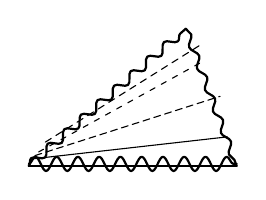
\begin{tikzpicture}[x=0.66cm,y=0.66cm,line cap=round,line join=round]
  \draw[thick] (0,0)--(4,0);
  \draw[thick,decorate,decoration={snake,amplitude=0.055cm,segment length=0.28cm}]
    (0,0)--(3.02,2.64);
  \draw[thick,decorate,decoration={snake,amplitude=0.041cm,segment length=0.29cm}]
    (3.02,2.64)--(4,0);
  \draw[thick,decorate,decoration={snake,amplitude=0.09cm,segment length=0.27cm}]
    (0,0.04)--(4,0.04);
  \draw (0.1,0.14)--(3.82,0.56);
  \draw[dash pattern=on 2.5pt off 1.6pt] (0.12,0.2)--(3.68,1.34);
  \draw[dash pattern=on 2pt off 2.6pt] (0.19,0.27)--(3.4,2.04);
  \draw[dash pattern=on 2.5pt off 2pt] (0.32,0.46)--(3.32,2.34);
\end{tikzpicture}}\endgroup
}
\end{GelfandAdjacentEvidence}
\begin{GelfandAdjacentEvidence}{GELFAND-P000949}{4}

есть 3-ник из 3-х геодезич.

Как его заполнить?

тоже геод. (отрезками)

Если в грассманиане сделать это, то не выходит.

Здесь получ.
\[
 \mathrm{Rank}\geqslant 2
\]
\SourceFigure{GELFAND-P000949}{rank-sign}{Знак между «Rank» и $2$ читается $\geqslant$.}
\end{GelfandAdjacentEvidence}
\begin{GelfandAdjacentEvidence}{GELFAND-P000949}{5}


(2) \underline{Опред.}\par
\underline{Гиперсимплекс $\Delta_n^m$}: мн-во точек
\[
 (x_1,\ldots,x_{n+m})\in\mathbb R^{n+m},
\]
удовл. соотн.
\begin{gather*}
 0\leq x_i\leq 1,\\
 \sum_i x_i=n
\end{gather*}
[после $n$ зачёркнуто: \sout{\mbox{\(+1\)}} (?)]
\Unclear{GELFAND-P000949}{hypersimplex-cancellation}{Штриховка закрывает запись после $n$. Чтение $+1$ предположительно; возможна буква $m$.}
\end{GelfandAdjacentEvidence}
\begin{GelfandAdjacentEvidence}{GELFAND-P000949}{6}


(3) \underline{Опр.}\qquad \uwave{Грассм. комплекс} в $P_{n+m-1}$:
выбир. $n+m$ точек $e_1,\ldots,e_{n+m}$, не леж. в гиперподпр-ве меньшей размер. (гиперплоскости).

$H^0$ = связная комп. $1$ подгруппы $PGL(n+m)$, к-рая ост. эти точки на месте.
\SourceFigure{GELFAND-P000949}{identity-component}{После «комп.» в рукописи стоит цифра $1$.}
\end{GelfandAdjacentEvidence}
\begin{GelfandAdjacentEvidence}{GELFAND-P000949}{7}


Грасм. комплекс --- замыкание орбиты \uwave{общ. полож.} группы $H^0$,
действующей на $G_n^m$.
[под «общ. полож.» написано \textit{generic}.]
\SourceFigure{GELFAND-P000949}{generic-gloss}{Английская помета стоит под волнистой чертой.}
\end{GelfandAdjacentEvidence}


(4) \underline{\textit{generic} --- ?}

это значит $H^0\xi$

$\xi$ --- подпр-во, трансверс. всем координ. подпр-вам:

если $e_1,\ldots,e_{n+m}$ принять за базис (какие-то точки на них)

это не то же самое, что $\dim=\max$ (!)

\Needspace{7\baselineskip}
\begin{GelfandAdjacentEvidence}{GELFAND-P000950}{1}
\SourcePage{GELFAND-P000950}{unlabelled}

(5) \underline{Теорема}. \uwave{Эти 2 объекта диффеоморфны.}

опр. (3) можно прив. для $\forall$ полупрост. группы.
\SourceFigure{GELFAND-P000950}{definition-verb}{Сокращение перед «для» читается «прив.».}
\end{GelfandAdjacentEvidence}
\begin{GelfandAdjacentEvidence}{GELFAND-P000950}{2}


$G_n^m$ --- $(n-1)$-подпр-ва в $P_{n+m-1}$ (?).
\Unclear{GELFAND-P000950}{projective-index}{Первый знак индекса густо переписан. Предположительно $P_{n+m-1}$; чтение $P_{m+n-1}$ не исключено.}
\end{GelfandAdjacentEvidence}
\begin{GelfandAdjacentEvidence}{GELFAND-P000950}{3}


(6) \underline{Пример}. \quad $\Delta_1^2\qquad G_1^2$

\SourceFigure{GELFAND-P000950}{cube-section}{Куб с заштрихованным сечением $H$. Внутренняя подпись, предположительно $x_3$, перекрыта линиями.
\par\smallskip
\begingroup\color{black}\GelfandFitDiagram{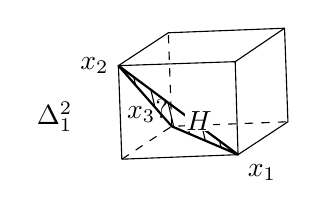
\begin{tikzpicture}[x=0.72cm,y=0.72cm,line join=round]
  \coordinate (o) at (0,0);
  \coordinate (x) at (2.05,0.08);
  \coordinate (y) at (-0.06,1.65);
  \coordinate (z) at (0.88,0.58);
  \coordinate (xy) at (2,1.72);
  \coordinate (xz) at (2.93,0.66);
  \coordinate (yz) at (0.82,2.23);
  \coordinate (xyz) at (2.87,2.31);
  \draw (o)--(x)--(xy)--(y)--cycle;
  \draw (y)--(yz)--(xyz)--(xy) (xyz)--(xz)--(x);
  \draw[dashed] (o)--(z)--(xz) (z)--(yz);
  \begin{scope}
    \clip (x)--(y)--(z)--cycle;
    \foreach \a in {0.3,0.55,...,1.8}{\draw[thin] (\a,0)--++(-0.4,1.7);}
  \end{scope}
  \draw[thick] (x)--(y)--(z)--cycle;
  \node[left] at (-0.7,0.75) {$\Delta_1^2$};
  \node[left] at (y) {$x_2$};
  \node[below right] at (x) {$x_1$};
  \node[above left,inner sep=1pt] at (z) {$x_3?$};
  \node[fill=white,inner sep=0.5pt] at (1.36,0.68) {$H$};
\end{tikzpicture}}\endgroup
}
\end{GelfandAdjacentEvidence}
\begin{GelfandAdjacentEvidence}{GELFAND-P000950}{4}


\SourceFigure{GELFAND-P000950}{projective-triangle}{Три прямые с отмеченными точками $e_1,e_2,e_3$. Римские номера и заштрихованная область показаны по рукописи.
\par\smallskip
\begingroup\color{black}\GelfandFitDiagram{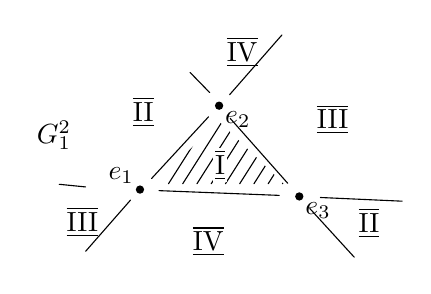
\begin{tikzpicture}[x=0.67cm,y=0.67cm,line cap=round]
  \coordinate (a) at (-1.42,-0.01);
  \coordinate (b) at (0.08,1.58);
  \coordinate (c) at (1.6,-0.14);
  \draw (-2.45,-1.18)--(-1.6,-0.21) (-1.2,0.2)--(-0.12,1.37) (0.28,1.79)--(1.27,2.92);
  \draw (-0.47,2.21)--(-0.1,1.83) (0.29,1.34)--(1.38,0.11) (1.8,-0.37)--(2.64,-1.29);
  \draw (-2.95,0.09)--(-2.45,0.04) (-1.06,-0.03)--(1.22,-0.12) (2,-0.16)--(3.55,-0.23);
  \begin{scope}
    \clip (-1.16,0.04)--(0.06,1.3)--(1.4,0.01)--cycle;
    \foreach \a in {-1.15,-0.88,...,1.3}{\draw[thin] (\a,0.1)--++(0.87,1.37);}
  \end{scope}
  \foreach \point in {a,b,c}{\fill (\point) circle[radius=1.5pt];}
  \node[above left,inner sep=2pt] at (a) {$e_1$};
  \node[below right,inner sep=2pt] at (b) {$e_2$};
  \node[below right,inner sep=2pt] at (c) {$e_3$};
  \node at (-3.05,1.02) {$G_1^2$};
  \node[fill=white,inner sep=0.7pt] at (0.1,0.46) {$\overline{\underline{\mathrm{I}}}$};
  \node at (-1.36,1.46) {$\overline{\underline{\mathrm{II}}}$};
  \node at (2.23,1.32) {$\overline{\underline{\mathrm{III}}}$};
  \node at (0.52,2.6) {$\overline{\underline{\mathrm{IV}}}$};
  \node at (-2.51,-0.62) {$\overline{\underline{\mathrm{III}}}$};
  \node at (2.92,-0.64) {$\overline{\underline{\mathrm{II}}}$};
  \node at (-0.12,-0.99) {$\overline{\underline{\mathrm{IV}}}$};
\end{tikzpicture}}\endgroup
}
\end{GelfandAdjacentEvidence}
\begin{GelfandAdjacentEvidence}{GELFAND-P000950}{5}


\uwave{преобр., сохр. и прямые}
\SourceFigure{GELFAND-P000950}{preserved-symbol}{После «сохр.» читается «и».}
\end{GelfandAdjacentEvidence}
\begin{GelfandAdjacentEvidence}{GELFAND-P000950}{6}


Внутр. $\Delta$-ка --- орбита (и связн. компонента соотв. подгр.)

(т.к. $PGL$ транзит. на 4-ках точек общего положения)

Всего --- 4 тр-ка

\SourceFigure{GELFAND-P000950}{hatched-simplex}{Малый заштрихованный треугольник с меткой I.
\par\smallskip
\begingroup\color{black}\GelfandFitDiagram{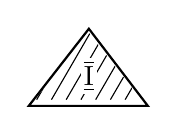
\begin{tikzpicture}[x=0.72cm,y=0.72cm]
  \draw[thick] (0,0)--(1.06,1.36)--(2.1,0)--cycle;
  \begin{scope}
    \clip (0.07,0.06)--(1.06,1.29)--(2.02,0.06)--cycle;
    \foreach \a in {0.14,0.4,...,1.95}{\draw[thin] (\a,0.11)--++(0.83,1.43);}
  \end{scope}
  \node[fill=white,inner sep=1pt] at (1.06,0.53) {$\overline{\underline{\mathrm{I}}}$};
\end{tikzpicture}}\endgroup
}
\end{GelfandAdjacentEvidence}
\begin{GelfandAdjacentEvidence}{GELFAND-P000950}{7}

--- пример грассм. симплекса

Есть гомеом., даже сохр. отметки (номера)
\SourceFigure{GELFAND-P000950}{preserved-segments}{Перед «(номера)» читается «отметки».}
\end{GelfandAdjacentEvidence}
\begin{GelfandAdjacentEvidence}{GELFAND-P000950}{8}


$\forall$ ребро --- симплекс в $G_1^1$

(7) \underline{Пример}. (другой !!).

$G_2^1$

\SourceFigure{GELFAND-P000950}{dual-orbit-diagram}{Пучки при трёх точках, наклонная секущая и штриховка. Слабые линии воссозданы приближённо.
\par\smallskip
\begingroup\color{black}\GelfandFitDiagram{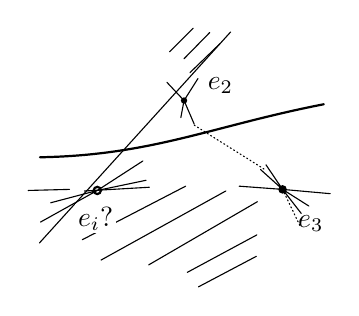
\begin{tikzpicture}[x=0.68cm,y=0.68cm,line cap=round]
  \coordinate (a) at (-1.45,0);
  \coordinate (b) at (0.17,1.68);
  \coordinate (c) at (2.01,0.02);
  \draw[thick] (-2.52,0.62) to[out=1,in=191] (2.78,1.61);
  \draw[thin] (-2.53,-0.98)--(1.04,2.96);
  \draw[thin] (-2.74,0)--(-1.97,0.02) (-1.69,-0.01)--(-0.48,0.06)
     (1.2,0.08)--(2.01,0.02)--(2.9,-0.06);
  \draw (-2.51,-0.59)--(a)--(-0.6,0.55) (-2.32,-0.23)--(a)--(-0.54,0.19);
  \draw (-0.15,2.02)--(b)--(0.36,1.24) (0.11,1.36)--(b)--(0.43,2.09);
  \draw (1.6,0.39)--(c)--(2.5,-0.29) (1.7,0.48)--(c)--(2.36,-0.43);
  \draw[thin,densely dotted] (0.36,1.22)--(1.68,0.39) (2.01,0.02)--(2.34,-0.67);
  \draw[thin] (-0.1,2.59)--(0.34,3.03) (0.17,2.46)--(0.65,2.95) (0.28,2.2)--(0.84,2.74);
  \draw[thin] (-1.73,-0.92)--(0.2,0.08) (-1.38,-1.3)--(0.95,-0.01)
     (-0.49,-1.39)--(1.54,-0.21) (0.23,-1.53)--(1.53,-0.83) (0.44,-1.8)--(1.52,-1.23);
  \draw[thick] (a) circle[radius=1.3pt];
  \fill (b) circle[radius=1.15pt] (c) circle[radius=1.55pt];
  \node[below,inner sep=1pt,fill=white] at (-1.48,-0.25) {$e_i?$};
  \node[right,inner sep=2pt] at (0.5,1.96) {$e_2$};
  \node[below right,inner sep=1pt] at (2.24,-0.4) {$e_3$};
\end{tikzpicture}}\endgroup
}
\end{GelfandAdjacentEvidence}
\begin{GelfandAdjacentEvidence}{GELFAND-P000950}{9}

\Unclear{GELFAND-P000950}{dual-left-index}{У левой нижней точки предположительно $e_i$; возможен индекс $1$.}
\end{GelfandAdjacentEvidence}
\begin{GelfandAdjacentEvidence}{GELFAND-P000950}{10}


орбита прямой --- $\forall$ прямых, не пересек. заштрих. область

Это $\Delta$-к --- со сторонами ---\par
--- прямые, прох. через вершины

\SourceFigure{GELFAND-P000950}{inverted-triangle}{Перевёрнутый треугольник с метками $13$, $23$ и обведённым $12$.
\par\smallskip
\begingroup\color{black}\GelfandFitDiagram{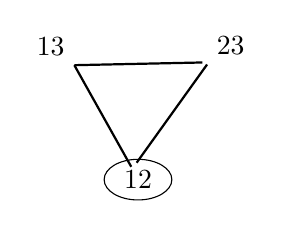
\begin{tikzpicture}[x=0.86cm,y=0.86cm]
  \draw[thick] (0,1.63)--(1.89,1.67) (1.96,1.64)--(0.92,0.19) (0.84,0.13)--(0,1.63);
  \node[above left] at (0,1.63) {$13$};
  \node[above right] at (1.96,1.64) {$23$};
  \draw (0.94,-0.06) ellipse (0.5 and 0.3);
  \node at (0.94,-0.06) {$12$};
\end{tikzpicture}}\endgroup
}
\end{GelfandAdjacentEvidence}
\begin{GelfandAdjacentEvidence}{GELFAND-P000950}{11}

--- соотв. стороне, прох. через $e_1$ и $e_2$.

\SourceFigure{GELFAND-P000950}{small-triangle-curves}{Треугольник с меткой $13$ и кривыми, пересекающими его стороны. Ход слабых кривых показан приближённо.
\par\smallskip
\begingroup\color{black}\GelfandFitDiagram{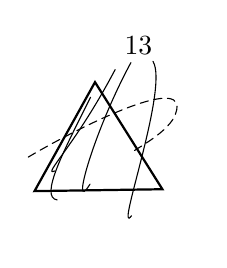
\begin{tikzpicture}[x=0.8cm,y=0.8cm,line cap=round]
  \draw[thick] (0,0)--(0.96,1.73)--(2.03,0.03)--cycle;
  \draw[thin] (0.36,-0.14) .. controls (0.07,-0.1) and (0.47,0.65) .. (0.89,1.49);
  \draw[thin] (0.32,0.32) .. controls (0.11,0.23) and (0.65,0.73) .. (1.28,1.93);
  \draw (0.88,0.11) .. controls (0.56,-0.41) and (0.93,0.93) .. (1.53,2.04);
  \draw (1.54,-0.39) .. controls (1.26,-0.77) and (2.14,1.65) .. (1.88,2.06);
  \draw[thin,densely dashed] (-0.1,0.54) .. controls (0.71,1.02) and (2.6,1.97) .. (2.21,1.16)
    .. controls (2.07,0.93) and (1.75,0.75) .. (1.58,0.64);
  \node[above] at (1.65,2.01) {$13$};
\end{tikzpicture}}\endgroup
}
\end{GelfandAdjacentEvidence}


\uwave{Стороны \mbox{\(\in G_1^1\)}} $\subset G_2^1$

$\Delta_2^1$ --- пересеч. куба с плоск. $\sum x_i=2$, причём вершины тоже обозначены парами.

\Needspace{7\baselineskip}
\begin{GelfandAdjacentEvidence}{GELFAND-P000951}{1}
\SourcePage{GELFAND-P000951}{52}

(8) \underline{Интересный} \underline{пример} $G_2^2$ \underline{или} $\Delta_2^2$

[на левом поле зачёркнуто: \sout{(9)} (?)]
\Unclear{GELFAND-P000951}{margin-top-cancellation}{Верхняя зачёркнутая помета похожа на «(9)»; возможно «(8)».}
\end{GelfandAdjacentEvidence}
\begin{GelfandAdjacentEvidence}{GELFAND-P000951}{2}

\[
 \sum_1^4 x_i=2\quad-\quad(\perp\ \text{гл. диаг. сечение 4-мерн. куба})
\]

[на левом поле зачёркнуто: знак не разобран]
\Unclear{GELFAND-P000951}{margin-diagram-cancellation}{Знак слева от рисунка закрыт несколькими штрихами.}
\end{GelfandAdjacentEvidence}
\begin{GelfandAdjacentEvidence}{GELFAND-P000951}{3}

\SourceFigure{GELFAND-P000951}{diagram-delta}{Размеченный рисунок $\Delta_2^2$. Слабые внутренние соединения показаны приближённо.
\par\smallskip
\begingroup\color{black}\GelfandFitDiagram{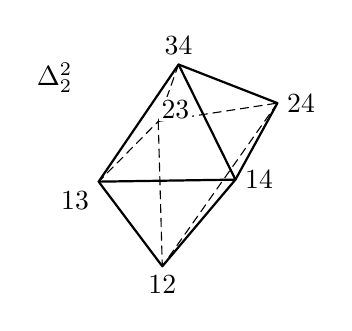
\begin{tikzpicture}[x=0.86cm,y=0.86cm,line join=round,line cap=round]
  \coordinate (t) at (0,3);
  \coordinate (u) at (1.46,2.43);
  \coordinate (v) at (0.84,1.3);
  \coordinate (w) at (-0.24,0.02);
  \coordinate (q) at (-1.18,1.27);
  \coordinate (h) at (-0.3,2.16);
  \draw[thick] (t)--(u)--(v)--(w)--(q)--cycle;
  \draw[thick] (q)--(v)--(t);
  \draw[densely dashed,thin] (t)--(h)--(q) (h)--(u) (h)--(w) (u)--(w);
  \node[above] at (t) {$34$};
  \node[right] at (u) {$24$};
  \node[right] at (v) {$14$};
  \node[below] at (w) {$12$};
  \node[below left] at (q) {$13$};
  \node[above right,fill=white,inner sep=1pt] at (h) {$23$};
  \node at (-1.83,2.8) {$\Delta_2^2$};
\end{tikzpicture}}\endgroup
}
\end{GelfandAdjacentEvidence}
\begin{GelfandAdjacentEvidence}{GELFAND-P000951}{4}


\begin{gather*}
 G_2^2\quad-\quad\text{4-мерно}\\
 H^0\quad-\quad\text{3-мерно}.
\end{gather*}

\SourceFigure{GELFAND-P000951}{diagram-four-planes}{Рисунок с точками $e_1,e_2,e_3,e_4$ и обозначением $\ell$. Слабые прерывистые штрихи показаны приближённо.
\par\smallskip
\begingroup\color{black}\GelfandFitDiagram{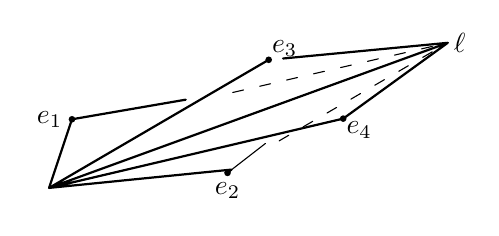
\begin{tikzpicture}[x=0.83cm,y=0.83cm,line join=round,line cap=round]
  \coordinate (o) at (0,0);
  \coordinate (e1) at (0.35,1.05);
  \coordinate (e2) at (2.73,0.23);
  \coordinate (e3) at (3.36,1.96);
  \coordinate (e4) at (4.5,1.06);
  \coordinate (l) at (6.1,2.22);
  \draw[thick] (o)--(e1)--(2.09,1.35);
  \draw[thick] (o)--(e3) (3.58,1.98)--(l) (o)--(l) (o)--(e4)--(l) (o)--(2.79,0.28)--(e2);
  \draw[thin] (e2)--(3.31,0.68);
  \draw[thin,dash pattern=on 4pt off 6pt] (2.81,1.46)--(l) (3.52,0.72)--(l);
  \foreach \point in {e1,e2,e3,e4}{\fill (\point) circle[radius=1.2pt];}
  \node[left] at (e1) {$e_1$};
  \node[below] at (e2) {$e_2$};
  \node[above right,inner sep=1pt] at (e3) {$e_3$};
  \node[below right,inner sep=1pt] at (e4) {$e_4$};
  \node[right,inner sep=2pt] at (l) {$\ell$};
\end{tikzpicture}}\endgroup
}
\end{GelfandAdjacentEvidence}
\begin{GelfandAdjacentEvidence}{GELFAND-P000951}{5}


$K(\ell)=\text{cross-ratio}$ 4-х плоскостей\par
\hspace{2em}(ангарм. отнош.) \quad прох. через $\ell$ и выбр. точки

(факторизуем всё по $\ell$ $\Rightarrow$ получ. в плоскости)
\[
 H^0\text{-орбита}\ \subset\ K(\ell)=\mathrm{const}
\]

\[
 \begin{array}{cc}
  \begin{gathered}
   G_2^2\\
   \cup\\
   G_2^2\supset
  \end{gathered}
  &
  \left\{\begin{array}{ccc|c}
   12&13&14&1\\
   21&23&24&2\\
   31&32&34&3\\
   41&42&43&4
  \end{array}\right.\\
  &\rule{11em}{0.3pt}\\
  \begin{gathered}
   G_2^1\supset\\
   \cap\\
   G_2^2
  \end{gathered}
  &
  \left\{\begin{array}{ccc|c}
   14&42&21&\phantom{1}\\
   13&32&21&\\
   14&43&31&\\
   24&43&32&
  \end{array}\right.
 \end{array}
\]
\SourceFigure{GELFAND-P000951}{table-upper-annotation}{Две верхние подписи читаются $G_2^2$, между ними U-образный знак.}
\end{GelfandAdjacentEvidence}
\begin{GelfandAdjacentEvidence}{GELFAND-P000951}{6}

\SourceFigure{GELFAND-P000951}{numerical-table}{Два блока рукописной таблицы с сохранённым порядком чисел.}
\end{GelfandAdjacentEvidence}
\begin{GelfandAdjacentEvidence}{GELFAND-P000951}{7}


Каждое --- в своём мн-зии (?) $K(\ell)=\mathrm{const}$
\Unclear{GELFAND-P000951}{below-table-abbreviation}{Сокращение после «своём» предположительно читается «мн-зии». Точное раскрытие не установлено.}
\end{GelfandAdjacentEvidence}
\begin{GelfandAdjacentEvidence}{GELFAND-P000951}{8}


(9) \underline{Теорема}. Объём мн-ва, закл., между 2-мя грассм. симплексами
\[
 K(\ell)=c_1,\quad K(\ell)=c_2
\]
равен
\[
 \Phi(c_1)-\Phi(c_2),
\]
\Unclear{GELFAND-P000951}{theorem-phi-difference}{Второй знак $\Phi$ переписан. Прежнее начертание неразборчиво.}
\end{GelfandAdjacentEvidence}

где
\[
 \Phi(x)=L_1(x)-L_1(1-x),\quad
 L_1(x)=\sum_{n=1}^{\infty}\frac{x^n}{n^2},\quad 0<c_1<c_2<1
\]
\hspace{6em}(интегр. логарифм)

\Needspace{7\baselineskip}
\begin{GelfandAdjacentEvidence}{GELFAND-P000952}{1}
\SourcePage{GELFAND-P000952}{unlabelled}

(10) \underline{Теорема}. Вообще говоря, [вписано над строкой: комбинаторный] гомеоморфизм
\SourceFigure{GELFAND-P000952}{combinatorial-insertion}{Надстрочное «комбинаторный» связано фигурной чертой с началом «гомеоморфизм».}
\end{GelfandAdjacentEvidence}
\begin{GelfandAdjacentEvidence}{GELFAND-P000952}{2}

\[
 \Delta_n^m\hookrightarrow \text{грассм. комплекс }G_n^m
\]
сохр. ещё ряд структур.

(11) [зачёркнуто: \underline{\sout{Теорема}}]
\SourceFigure{GELFAND-P000952}{theorem-cancellation}{Под штриховкой читается подчёркнутое «Теорема».}
\end{GelfandAdjacentEvidence}
\begin{GelfandAdjacentEvidence}{GELFAND-P000952}{3}

\SourceFigure{GELFAND-P000952}{faces-orbits-diagram}{Схема соответствия граней и $H^0$-орбит. Под «орбиты» штрих без видимого наконечника.
\par\smallskip
\begingroup\color{black}\GelfandFitDiagram{\begin{tikzpicture}[x=0.82cm,y=0.82cm]
  \node (faces) at (0,0) {Грани};
  \node[above left,inner sep=0.8pt] (interior) at (faces.north) {\scriptsize внутр.};
  \draw[thin] (interior.south west) to[out=-30,in=155] (faces.north west);
  \node (orbits) at (3.65,0) {$H^0$-[?] орбиты};
  \draw[->] (1.05,0.14) to[out=202,in=177] (2.34,0.02);
  \node[above] at (1.68,0.2) {\scriptsize соотв.};
  \draw (orbits.south)--++(0,-0.34);
  \node[below,inner sep=1pt] at (3.65,-0.63) {лежат в $G_i^j$};
\end{tikzpicture}}\endgroup
}
\end{GelfandAdjacentEvidence}
\begin{GelfandAdjacentEvidence}{GELFAND-P000952}{4}

\Unclear{GELFAND-P000952}{faces-orbits-cancellation}{Запись после $H^0$ и дефиса зачёркнута и не разобрана.}
\end{GelfandAdjacentEvidence}
\begin{GelfandAdjacentEvidence}{GELFAND-P000952}{5}


(12)
\begin{align*}
 \partial[\Delta_n^m]
 &=\sum_{i=1}^{n+m}(-1)^i\bigl\{[\Delta_n^{m-1}]\mid i\text{-я коорд.}=0\bigr\}-\\
 &-\sum_{-1}^{n+m}(-1)^i\bigl\{[\Delta_{n-1}^{m}]
\end{align*}
\Incomplete{GELFAND-P000952}{boundary-formula-second-line}{Во второй сумме нижний предел читается $-1$. Запись обрывается после $[\Delta_{n-1}^{m}]$.}
\end{GelfandAdjacentEvidence}
\begin{GelfandAdjacentEvidence}{GELFAND-P000952}{6}


(13) \underline{Теорема}. $\forall$ гарм. форма в $G_n^m$ обращ. в $0$ на любом грассм. симплексе.

Метрика предпол. нек-рым обр. соглас. с координатами.

\SourceFigure{GELFAND-P000952}{metric-diagram}{Фигурная скобка под списком ведёт к базису. Под «метрика» виден штрих без наконечника.
\par\smallskip
\begingroup\color{black}\GelfandFitDiagram{\begin{tikzpicture}[x=0.8cm,y=0.8cm]
  \node (coords) at (0,0) {$\underbrace{e_i,\ldots,e_{n+m}}$};
  \node (metric) at (3.55,0) {метрика};
  \draw[->] (1.27,0.17) to[out=202,in=174] (2.58,0.02);
  \draw[->] (0,-0.43)--(0,-0.8);
  \node[below,inner sep=1pt] at (0,-0.88) {ортог. базис (?)};
  \draw (metric.south)--++(0,-0.34);
  \node[below,inner sep=1pt] at (3.55,-0.68) {$O(n+m)$};
\end{tikzpicture}}\endgroup
}
\end{GelfandAdjacentEvidence}
\begin{GelfandAdjacentEvidence}{GELFAND-P000952}{7}

\SourceFigure{GELFAND-P000952}{metric-first-index}{Под первым $e$ виден индекс $i$ с точкой.}
\end{GelfandAdjacentEvidence}
\begin{GelfandAdjacentEvidence}{GELFAND-P000952}{8}

\Unclear{GELFAND-P000952}{metric-basis-abbreviation}{Сокращение предположительно «ортог.»; возможно «ортон.».}
\end{GelfandAdjacentEvidence}
\begin{GelfandAdjacentEvidence}{GELFAND-P000952}{9}


\underline{О работе Атьи.}
\SourceFigure{GELFAND-P000952}{atiyah-name}{Фамилия записана «Атьи».}
\end{GelfandAdjacentEvidence}
\begin{GelfandAdjacentEvidence}{GELFAND-P000952}{10}

\uwave{Отсюда функц. ур-е для дилогарифма}.

Пр-во 5-к точек на $P^1$ с точн. до проект. преобр.
\SourceFigure{GELFAND-P000952}{five-points-line}{Прямая с пятью подписями и неподписанным штрихом справа. Утолщённый конец показан приближённо.
\par\smallskip
\begingroup\color{black}\GelfandFitDiagram{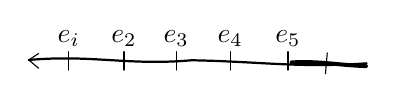
\begin{tikzpicture}[x=0.78cm,y=0.78cm,line cap=round]
  \draw[thick] (0,0.015) to[out=5,in=185] (2.65,0.01) to[out=-1,in=184] (5.5,-0.04);
  \draw (0.16,0.12)--(0,0.015)--(0.16,-0.12);
  \foreach \position/\pointindex in {0.65/i,1.55/2,2.4/3,3.28/4,4.22/5}{
    \draw (\position,-0.15)--(\position,0.15);
    \node[above,inner sep=1pt] at (\position,0.18) {$e_{\pointindex}$};
  }
  \draw[line width=1.45pt] (4.28,-0.025) to[out=3,in=178] (5.49,-0.085);
  \draw (4.83,-0.21)--(4.86,0.13);
\end{tikzpicture}}\endgroup
}
\end{GelfandAdjacentEvidence}
\begin{GelfandAdjacentEvidence}{GELFAND-P000952}{11}

\SourceFigure{GELFAND-P000952}{five-points-first-index}{У первого $e$ подписано $i$ с точкой.}
\end{GelfandAdjacentEvidence}
\begin{GelfandAdjacentEvidence}{GELFAND-P000952}{12}

Это пр-во 2-мерно.

\begin{align*}
 k_1&=\text{X ratio}\;(e_2\,e_3\,e_4\,e_5)\\
 k_2&=\text{--- '' ---}\;(e_1\,e_3\,e_4\,e_5)
\end{align*}
\Unclear{GELFAND-P000952}{cross-ratio-sign}{Знак перед «ratio» предположительно читается как $X$. Начертания $X$ и $\times$ близки.}
\end{GelfandAdjacentEvidence}

$\cdots$
\[
 \varphi(x)=\operatorname{Li}(x)-\operatorname{Li}(1-x),\qquad
 \operatorname{Li}(x)=\sum_1^\infty\frac{x^n}{n^2}.
\]

\begin{equation*}
 0=d\varphi(k_1)-d\varphi(k_2)+d\varphi(k_3)-d\varphi(k_4)+d\varphi(k_5)
 \tag{14}
\end{equation*}
(Функц. ур-е для дилогарифма)

Это следует из ранее сформ. теорем.

$G_3^2$ --- 3-мер. плоск. в $\mathbb R^5$.

Рассм. $P_1(\xi)$ (1-й класс Понтрягина тавтологич. 2 или 3-мерн. рассл. на Грассм. $G_3^2$).

Есть ровно 1 гармонич. 4-форма.

\Needspace{7\baselineskip}
\begin{GelfandAdjacentEvidence}{GELFAND-P000953}{1}
\SourcePage{GELFAND-P000953}{53}

\[
 \underset{\substack{\Vert\\0}}{d}\pi_*P_1(\xi)
 =\pi_*\underset{\substack{\Vert\\0}}{d}P_1(\xi)
 +\sum\pi_{i*}^{\partial}P_1(\xi)
\]
\SourceFigure{GELFAND-P000953}{zeros-under-formula}{Под каждым из двух $d$ записаны две черты и нуль.}
\end{GelfandAdjacentEvidence}
\begin{GelfandAdjacentEvidence}{GELFAND-P000953}{2}

$C$ --- пр-во 5-к точек

\SourceFigure{GELFAND-P000953}{top-projection}{Знак слева от $\subset$ похож на строчное $u$; возможна прописная $U$.
\par\smallskip
\begingroup\color{black}\GelfandFitDiagram{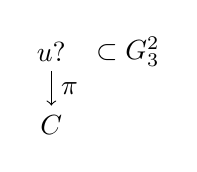
\begin{tikzpicture}[x=0.83cm,y=0.83cm]
  \node (u) at (0,0) {$u?$};
  \node at (1.17,0) {$\subset G_3^2$};
  \node (c) at (0,-1.12) {$C$};
  \draw[->] (u.south)--node[right] {$\pi$} (c.north);
\end{tikzpicture}}\endgroup
}
\end{GelfandAdjacentEvidence}
\begin{GelfandAdjacentEvidence}{GELFAND-P000953}{3}


Последн. член вычисл. с пом. комбинаторики
\SourceFigure{GELFAND-P000953}{combinatorics-wording}{Перед «комбинаторики» записано «с пом.».}
\end{GelfandAdjacentEvidence}
\begin{GelfandAdjacentEvidence}{GELFAND-P000953}{4}


\underline{Обобщение}.

Пусть $(\mathbb C^*)^n$ алгебраически действ. на однородном алгебр. [зачёркнуто: запись не разобрана] пр-ве с неподв. точкой
\Incomplete{GELFAND-P000953}{generalization-cancellation}{Запись между «алгебр.» и «пр-ве» густо зачёркнута.}
\end{GelfandAdjacentEvidence}
\begin{GelfandAdjacentEvidence}{GELFAND-P000953}{5}


Тогда

1) $\forall$ орбита $\bigl((\mathbb R^+)^*\bigr)^n$ гомеом. полиэдру.
(теорема о торических вложениях)

(Диффеом. на $\forall$ орбите, но в верш. может иметь $\infty$ кривизну; на всём --- лишь гомеом.)

2) $\forall$ гарм. форма [зачёркнуто: запись не разобрана]
инвар. отн. $T^n\subset(\mathbb C^*)^n$
\Incomplete{GELFAND-P000953}{harmonic-cancellation}{Запись после «форма» закрыта несколькими штрихами.}
\end{GelfandAdjacentEvidence}
\begin{GelfandAdjacentEvidence}{GELFAND-P000953}{6}

[под «гарм. форма» вписано: (по отн. к $\forall$ Кэлеровой метрике)]
\SourceFigure{GELFAND-P000953}{kahler-insertion}{Условие о метрике записано строкой ниже.}
\end{GelfandAdjacentEvidence}
\begin{GelfandAdjacentEvidence}{GELFAND-P000953}{7}

равна $0$ на $\forall$ $\bigl((\mathbb R^+)^*\bigr)^n$-орбите.

(15) \underline{Теорема}. (Атья).

$M$ --- симплектич. мн-зие, $f_1,\ldots,f_n\colon M\longrightarrow\mathbb R$ функции.
\SourceFigure{GELFAND-P000953}{symplectic-abbrev}{Сокращение после «симплектич.» читается «мн-зие».}
\end{GelfandAdjacentEvidence}
\begin{GelfandAdjacentEvidence}{GELFAND-P000953}{8}

\[
 \{f_i,f_j\}=0
\]

$df_i$ все обр. в $0$ в \underline{нек-рой точке}.

Получ. отобр.
\[
 M\underset{f_1,\ldots,f_n}{\longrightarrow}\mathbb R^n
\]
При этом

\SourceFigure{GELFAND-P000953}{orbit-image}{От $O$ идёт стрелка к выпуклому множеству. Ниже $O$ стоит черта к подписи об орбите.
\par\smallskip
\begingroup\color{black}\GelfandFitDiagram{\begin{tikzpicture}[x=0.79cm,y=0.79cm]
  \node (orb) at (0,0) {$O$};
  \draw[->] (0.52,0.05) to[out=-11,in=192] (1.78,0.04);
  \node[anchor=west,align=left,text width=4.7cm] (target) at (1.92,0)
    {выпуклое мн-во, имеющее конечное число вершин\\(т.е. многогранник).};
  \coordinate (flowtop) at (orb.center |- target.south);
  \node[anchor=north west,align=left,text width=5.25cm,inner sep=1pt] (flow) at ([xshift=-1.2mm,yshift=-3mm]flowtop) {орбита потока, заданного полями $H_{f_i}$};
  \draw (orb.south)--(orb.south |- flow.north);
\end{tikzpicture}}\endgroup
}
\end{GelfandAdjacentEvidence}
\begin{GelfandAdjacentEvidence}{GELFAND-P000953}{9}


\SourceFigure{GELFAND-P000953}{divider-strokes}{Две черты с точкой между ними.
\par\smallskip
\begingroup\color{black}\GelfandFitDiagram{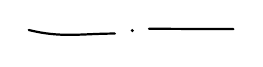
\begin{tikzpicture}[x=0.76cm,y=0.76cm,line cap=round]
  \draw[thick] (0,0.06) to[out=-14,in=180] (1.44,0);
  \fill (1.73,0.05) circle[radius=0.62pt];
  \draw[thick] (2.01,0.08)--(3.42,0.075);
\end{tikzpicture}}\endgroup
}
\end{GelfandAdjacentEvidence}


\underline{Задача}: связь с интегр. в квадратурах.

\clearpage
\pdfbookmark[0]{Глава 19}{gelfand-archive-chapter-19}
\section*{Глава 19}
\Needspace{7\baselineskip}
\begin{GelfandAdjacentEvidence}{GELFAND-P000954}{1}
\SourcePage{GELFAND-P000954}{unlabelled}

16/\(\overline{\underline{\mathrm{II}}}\)-81 г.\quad \underline{Сем. Гельфанда.}
\SourceFigure{GELFAND-P000954}{date-hatching}{Дата подчёркнута узкой заштрихованной полосой. У II черты сверху и снизу.
\par\smallskip
\begingroup\color{black}\GelfandFitDiagram{\begin{tikzpicture}[x=0.81cm,y=0.81cm,line join=round]
  \node[above,inner sep=2pt] at (1.65,0.11) {16/\(\overline{\underline{\mathrm{II}}}\)-81 г.};
  \draw[thick] (0,0)--(0.14,0.17)--(3.3,0.13)--(3.35,-0.035)--(1.82,-0.03)--(0.67,0.02)--cycle;
  \foreach \x in {0.16,0.37,...,3.2}{\draw[thin] (\x,0.008)--++(-0.075,0.127);}
\end{tikzpicture}}\endgroup
}
\end{GelfandAdjacentEvidence}
\begin{GelfandAdjacentEvidence}{GELFAND-P000954}{2}


\underline{\underline{Хованский}}. \quad \underline{О многогранниках Ньютона}.

[Справа: (оборотная сторона пред. докл. Mc Pherson’а.)]
\SourceFigure{GELFAND-P000954}{verso-note}{Помета о том, что запись сделана на обороте предыдущего доклада.}
\end{GelfandAdjacentEvidence}
\begin{GelfandAdjacentEvidence}{GELFAND-P000954}{3}


$\underline{\underline{n=2}}$ \uwave{для простоты}.

\underline{лит-ра}: 1) Mumford и др. Lect. Notes --- торические вложения.

2) Д. Бернштейн, ФА.

1) Kempf, Knudsen, Mumford, Saint-Donat, Toroidal Embeddings,

Lect. Notes Math., 1972, $N=339$.
\SourceFigure{GELFAND-P000954}{printed-year}{В рукописной ссылке указаны 1972 год и номер 339.}
\end{GelfandAdjacentEvidence}


\Needspace{7\baselineskip}
\begin{GelfandAdjacentEvidence}{GELFAND-P000955}{1}
\SourcePage{GELFAND-P000955}{unlabelled}

и ещё обзор \uwave{Данилова} в УМН.

Ст. \uwave{Хованского}: ФА, 1977, 11:4\par
\hspace{4em}1978, 12:1

\begin{equation*}
 \{(x,y):P(x,y)=0\}
 \tag{1}
\end{equation*}
как выглядит эта кривая? (ручки и т. д.)

Сколько решений имеет система
\begin{equation*}
 \begin{cases}
 P(x,y)=0\\
 Q(x,y)=0
 \end{cases}
 \tag{2}
\end{equation*}
[зачёркнуто: (строка не разобрана).]
\Incomplete{GELFAND-P000955}{cancelled-line}{Строка в скобках густо зачёркнута.}
\end{GelfandAdjacentEvidence}
\begin{GelfandAdjacentEvidence}{GELFAND-P000955}{2}


\begin{equation*}
 y^2=P_n(x)
 \tag{3}
\end{equation*}
имеет $\sim n/2$ ручек (точнее, $\left[\frac{n-1}{2}\right]$ ручек).
\begin{gather*}
 n=3,4\qquad 1\text{ ручка},\\
 n=5,6\qquad 2\text{ ручки}.
\end{gather*}
Условие: $P_n$ не имеет кратных корней.

Для общего ур-я (1) тоже есть рецепт вычисления числа ручек:
\begin{equation*}
 \frac{(n-1)(n-2)}{2}\qquad\text{\uwave{для ур-я общего положения.}}
 \tag{4}
\end{equation*}
(3) --- не ур-е степени $n$ на самом деле.
\SourceFigure{GELFAND-P000955}{degree-remark}{Фраза о степени (3) приведена в том виде, в каком записана в рукописи.}
\end{GelfandAdjacentEvidence}
\begin{GelfandAdjacentEvidence}{GELFAND-P000955}{3}


Всё дело --- в многогр. Ньютона.
\begin{equation*}
 P(x,y)=\sum a_{n,k}x^n y^k.
 \tag{5}
\end{equation*}
\SourceFigure{GELFAND-P000955}{newton-triangle}{Треугольник со штриховкой, оси $k,n$ и отметки. Подпись над $2$ зачёркнута.
\par\smallskip
\begingroup\color{black}\GelfandFitDiagram{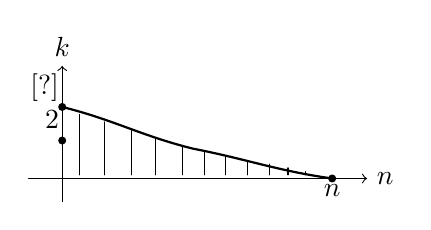
\begin{tikzpicture}[x=0.79cm,y=0.79cm,line cap=round]
  \draw[->] (-0.54,0)--(4.9,0) node[right] {$n$};
  \draw[->] (0,-0.37)--(0,1.81) node[above] {$k$};
  \draw[thick] (0,1.15) to[out=-14,in=166] (2.1,0.48) to[out=-11,in=172] (4.34,0);
  \foreach \x/\h in {0.28/1.03,0.68/0.91,1.12/0.77,1.5/0.65,1.94/0.53,2.29/0.44,2.63/0.36,2.98/0.29,3.33/0.23,3.63/0.17,3.91/0.11}{
    \draw[thin] (\x,0.06)--(\x,\h);
  }
  \fill (0,0.61) circle[radius=1.45pt] (0,1.15) circle[radius=1.45pt] (4.34,0) circle[radius=1.45pt];
  \node[below left,inner sep=1pt] at (0,1.15) {$2$};
  \node[left,inner sep=1pt] at (0,1.46) {$[\text{?}]$};
  \node[below,inner sep=2pt] at (4.34,0) {$n$};
\end{tikzpicture}}\endgroup
}
\end{GelfandAdjacentEvidence}
\begin{GelfandAdjacentEvidence}{GELFAND-P000955}{4}

\Incomplete{GELFAND-P000955}{triangle-cancelled-label}{Густо зачёркнутая подпись над $2$ не разобрана.}
\end{GelfandAdjacentEvidence}
\begin{GelfandAdjacentEvidence}{GELFAND-P000955}{5}


\uwave{Вып. оболочка} тех $(n,k)$, для к-рых $a_{nk}\ne0$.

\SourceFigure{GELFAND-P000955}{general-simplex}{Второй треугольник, с четырьмя внутренними штрихами.
\par\smallskip
\begingroup\color{black}\GelfandFitDiagram{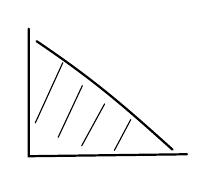
\begin{tikzpicture}[x=0.83cm,y=0.83cm,line cap=round]
  \draw[thick] (0,1.95)--(0,0)--(2.42,0.03);
  \draw[thick] (0.12,1.76) to[out=-34,in=138] (2.2,0.1);
  \draw (0.1,0.51)--(0.52,1.43) (0.45,0.29)--(0.82,1.08)
        (0.81,0.16)--(1.16,0.8) (1.31,0.09)--(1.56,0.56);
\end{tikzpicture}}\endgroup
}
\end{GelfandAdjacentEvidence}
\begin{GelfandAdjacentEvidence}{GELFAND-P000955}{6}

--- \uwave{общ. случай} --- симплекс.

Ответ для (1) --- [над строкой вписано: \uwave{число ручек} $=$]
\uwave{число целых внутр. точек в многогр. Ньют.}
\SourceFigure{GELFAND-P000955}{genus-insertion}{«число ручек» и знак равенства вписаны над ответом.}
\end{GelfandAdjacentEvidence}


(для коэфф. $a_{n,k}$ общего положения)

Это теор. \uwave{Бейкера} (того самого), переоткрыта Хованским в 1976 г.

(Бейкер --- учитель Ходжа, Ходж --- учитель Атьи)

В $\mathbb C^2$ не все точки кривой (1) видны. Хотим их проявить нек-рыми заменами.

Рассм. кривую $P(x,y)=0$ \uwave{вне коорд. креста}.

$x,y$ --- мероморфные ф-и на рим. пов.

Иногда они обр. в $0$ или $\infty$. Это даёт дивизор:

в $\forall$ его точке есть вектор $(n,m)$

(порядок нуля $x=n$, порядок нуля $y=m$ в данной точке)

\Needspace{7\baselineskip}
\begin{GelfandAdjacentEvidence}{GELFAND-P000956}{1}
\SourcePage{GELFAND-P000956}{6}

Точки порядка $(1,0)$ или $(k,0)$ видны на картинке: это точки пересеч. с осью \underline{$x=0$}.

Можем паралл. переносить многоуг. умножением на $x^k$ и $y^k$.

\SourceFigure{GELFAND-P000956}{axis-polygon}{Пятиугольник касается оси $y$ ребром, а оси $x$ вершиной.
\par\smallskip
\begingroup\color{black}\GelfandFitDiagram{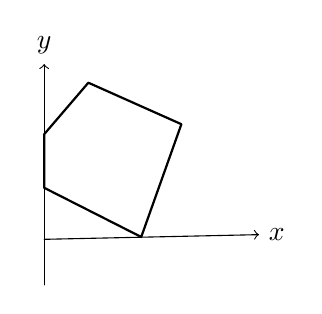
\begin{tikzpicture}[x=0.85cm,y=0.85cm,line cap=round,line join=round]
  \draw[->] (0,-0.68)--(0,2.62) node[above] {$y$};
  \draw[->] (0,0)--(3.21,0.07) node[right] {$x$};
  \draw[thick] (0,0.77)--(0,1.57)--(0.66,2.34)--(2.05,1.72)--(1.45,0.035)--cycle;
\end{tikzpicture}}\endgroup
}
\end{GelfandAdjacentEvidence}
\begin{GelfandAdjacentEvidence}{GELFAND-P000956}{2}


Перенесём, чтобы коснулся оси $x=0$.
\begin{equation*}
 P(0,y)=0
 \tag{6}
\end{equation*}
Число реш. $=$ \uwave{длина отрезка пересечения} МН с осью $\{x=0\}$.

(если нет кратных корней

\SourceFigure{GELFAND-P000956}{transverse-branches}{Три ветви пересекают вертикальную линию с подписью $x=0$.
\par\smallskip
\begingroup\color{black}\GelfandFitDiagram{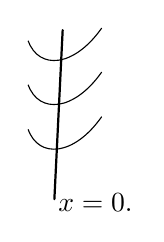
\begin{tikzpicture}[x=0.81cm,y=0.81cm,line cap=round]
  \draw[thick] (-0.07,0)--(0.06,2.65);
  \foreach \level in {0.95,1.65,2.34}{
    \draw (-0.48,\level+0.14) .. controls (-0.31,\level-0.32) and (0.24,\level-0.27) .. (0.67,\level+0.34);
  }
  \node[below right,inner sep=1pt] at (-0.06,0.14) {\uwave{\mbox{\(x=0\)}}.};
\end{tikzpicture}}\endgroup
}
\end{GelfandAdjacentEvidence}
\begin{GelfandAdjacentEvidence}{GELFAND-P000956}{3}

некратные $\Rightarrow$ теор. о неявной ф-и применима

$\Rightarrow$ нет точек вида $(k,0)$, $k\geqslant2$.

\uwave{Сделаем преобр.}
\begin{equation*}
 \begin{cases}
 x=u^{a_{11}}v^{a_{12}},\\
 y=u^{a_{21}}v^{a_{22}},
 \end{cases}
 \qquad a_{ij}\in\mathbb Z
 \tag{7}
\end{equation*}
\begin{equation*}
 \det\begin{Vmatrix}a_{11}&a_{12}\\a_{21}&a_{22}\end{Vmatrix}=1,
 \qquad A=\begin{pmatrix}a_{11}&a_{12}\\a_{21}&a_{22}\end{pmatrix}.
 \tag{8}
\end{equation*}
обратная --- целочисл. $\Rightarrow$ есть обратное преобр. (тоже рацион.)

Если $u\sim t^m$, $v\sim t^n$, то после преобразования
\begin{equation*}
 \operatorname{ord}\left(\text{[зач.]}\ \begin{matrix}x\\y\end{matrix}\right)
 =A\ \text{[зач.]}\begin{pmatrix}m\\n\end{pmatrix}.
 \tag{9}
\end{equation*}
\Unclear{GELFAND-P000956}{order-formula}{Знаки слева от столбца $x,y$ и после $A$ густо зачёркнуты. Оба похожи на $u$, но точное чтение не установлено.}
\end{GelfandAdjacentEvidence}
\begin{GelfandAdjacentEvidence}{GELFAND-P000956}{4}


Хотим сделать такое преобр., чтобы в т. $\binom{n}{m}$ попал $\binom{1}{0}$.

Пусть вектор $(n,m)$ несократим ($\sim$ на отрезке $[0,(m,n)]$ нет целых точек).
\Unclear{GELFAND-P000956}{primitive-vector}{Первый знак в паре густо переписан; предположительно $n$. В следующей записи порядок букв $(m,n)$.}
\end{GelfandAdjacentEvidence}
\begin{GelfandAdjacentEvidence}{GELFAND-P000956}{5}


\uwave{Мораль}: $\exists$ матрица $A$.

Если [зачёркнуто: \sout{он} (?); над строкой вписано: $(n,m)$] сократим, то это же преобр. показывает, что \underline{дивизоров таких нет}!!
\Unclear{GELFAND-P000956}{substituted-vector}{Над зачёркнутым словом, предположительно «он», вписано $(n,m)$.}
\end{GelfandAdjacentEvidence}
\begin{GelfandAdjacentEvidence}{GELFAND-P000956}{6}


\underline{ответ}.

\SourceFigure{GELFAND-P000956}{vertex-support}{Одна из параллельных прямых касается вершины пятиугольника. От отмеченной точки на другой прямой проведена стрелка $(n,m)$.
\par\smallskip
\begingroup\color{black}\GelfandFitDiagram{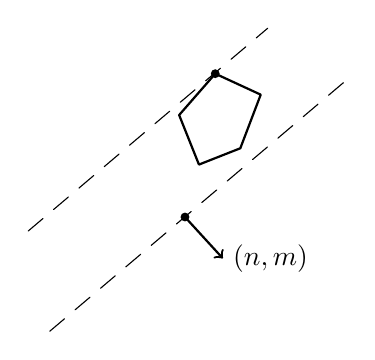
\begin{tikzpicture}[x=0.74cm,y=0.74cm,line cap=round,line join=round]
  \coordinate (v) at (1.55,2.67);
  \coordinate (o) at (1.03,0.21);
  \draw[thin,dash pattern=on 7pt off 5pt] (-1.66,-0.03)--(2.45,3.45);
  \draw[thick] (v)--(2.33,2.31)--(1.98,1.39)--(1.27,1.11)--(0.93,1.96)--cycle;
  \draw[thin,dash pattern=on 7pt off 5pt] (-1.29,-1.75)--(3.79,2.55);
  \fill (v) circle[radius=1.6pt] (o) circle[radius=1.6pt];
  \draw[thick,->] (o)--(1.68,-0.5) node[right] {$(n,m)$};
\end{tikzpicture}}\endgroup
}
\end{GelfandAdjacentEvidence}
\begin{GelfandAdjacentEvidence}{GELFAND-P000956}{7}


\uwave{двигаем, пока не коснётся}

[зачёркнуто: \sout{если} (?)] Наткнулись на точку ---\par
--- тогда таких нет.
\Unclear{GELFAND-P000956}{cancelled-word}{Зачёркнутое слово предположительно читается «если».}
\end{GelfandAdjacentEvidence}
\begin{GelfandAdjacentEvidence}{GELFAND-P000956}{8}


\SourceFigure{GELFAND-P000956}{edge-support}{У шестиугольника выделено левое ребро, лежащее на наклонной прямой. Справа параллельная прямая.
\par\smallskip
\begingroup\color{black}\GelfandFitDiagram{\begin{tikzpicture}[x=0.74cm,y=0.74cm,line cap=round,line join=round]
  \coordinate (a) at (0.18,0.81);
  \coordinate (b) at (0.82,1.92);
  \draw[thin] (-0.73,-0.78)--(b);
  \draw[thin,dash pattern=on 8pt off 6pt] (1.74,-1.06)--(3.82,2.54);
  \draw[thick] (a)--(b)--(1.85,2.04)--(2.58,1.46)--(1.94,0.36)--(1.17,0.28)--cycle;
  \draw[line width=1.2pt] (a)--(b);
\end{tikzpicture}}\endgroup
}
\end{GelfandAdjacentEvidence}
\begin{GelfandAdjacentEvidence}{GELFAND-P000956}{9}

$\leftarrow$ тогда получ. $=$ числу целых точек на этом отрезке.
\SourceFigure{GELFAND-P000956}{final-count}{В последней строке сказано «числу целых точек на этом отрезке».}
\end{GelfandAdjacentEvidence}


(берём $\min$ скал. произведения)

\Needspace{7\baselineskip}
\begin{GelfandAdjacentEvidence}{GELFAND-P000957}{1}
\SourcePage{GELFAND-P000957}{unlabelled}

\uwave{Общее число проколов} $=$ числу целочисл. точек на границе.

Рассмотрим теперь систему
\begin{equation*}
 \begin{cases}
 P(x,y)=0\\
 Q(x,y)=0
 \end{cases}
 \tag{10}
\end{equation*}
и ищем число реш. в $(\mathbb C\setminus0)^2$

([зачёркнуто: не разобрано] $x\ne0,\infty$; $y\ne0,\infty$).
\Unclear{GELFAND-P000957}{cancelled-before-conditions}{Короткая запись перед условием на $x$ закрыта зачёркиванием.}
\end{GelfandAdjacentEvidence}
\begin{GelfandAdjacentEvidence}{GELFAND-P000957}{2}


Рассм. ф-ю $Q$ на кривой $P(x,y)=0$.

Её дивизор $=0$,
\SourceFigure{GELFAND-P000957}{divisor-zero}{В рукописи записано «Её дивизор $=0$».}
\end{GelfandAdjacentEvidence}
\begin{GelfandAdjacentEvidence}{GELFAND-P000957}{3}

Смотрим порядок в выкин. точках!!

$(n,m)$\qquad $x\sim t^n$, $y\sim t^m$.

Тогда
\begin{equation*}
 \sum C_{a,b}x^a y^b=C_{a,b}t^{an+bm}
 \tag{11}
\end{equation*}
\SourceFigure{GELFAND-P000957}{expansion-eleven}{В (11) знак суммы стоит слева от равенства.}
\end{GelfandAdjacentEvidence}
\begin{GelfandAdjacentEvidence}{GELFAND-P000957}{4}


\underline{ответ}:
\begin{equation*}
 \underline{\underline{\min_{a,b}\bigl((n,m)\cdot(a,b)\bigr)}}
 \qquad\text{--- \uwave{чисто геом. ответ}.}
 \tag{12}
\end{equation*}
Выколотые точки --- на кресте или в $\infty$

$\Rightarrow$ \uwave{полюса только в выколотых точках}.
\begin{equation*}
 \left[\sum_{m,n}(12)\right]
 =\text{числу реш. (10) в [зачёркнуто: \sout{пространстве} (?)] }(\mathbb C\setminus0)^2.
 \tag{13}
\end{equation*}
\Unclear{GELFAND-P000957}{thirteen-cancellation}{Перед $(\mathbb C\setminus0)^2$ предположительно зачёркнуто «пространстве».}
\end{GelfandAdjacentEvidence}
\begin{GelfandAdjacentEvidence}{GELFAND-P000957}{5}

\SourceFigure{GELFAND-P000957}{thirteen-sign}{В (13) перед знаком суммы нет минуса.}
\end{GelfandAdjacentEvidence}
\begin{GelfandAdjacentEvidence}{GELFAND-P000957}{6}


(для общ. полож. --- иначе сократиться может).

Есть 2 многоугольника!! Что получается?

\underline{Ответ} --- смешанный объём!!

Складываем все вект. $(n,m)$ --- получим вектор длиной $=$ длине стороны.

\SourceFigure{GELFAND-P000957}{normal-arrows}{Три стрелки последовательно направлены вниз и вправо.
\par\smallskip
\begingroup\color{black}\GelfandFitDiagram{\begin{tikzpicture}[x=0.87cm,y=0.87cm,line cap=round]
  \draw[very thick,->] (0,1.53)--(0.24,1.02);
  \draw[very thick,->] (0.24,1.02)--(0.46,0.47);
  \draw[very thick,->] (0.46,0.47)--(0.59,-0.06);
\end{tikzpicture}}\endgroup
}
\end{GelfandAdjacentEvidence}
\begin{GelfandAdjacentEvidence}{GELFAND-P000957}{7}


Вектор $\perp$ стороне и равный ей по длине.

\uwave{Пусть 2 многоуг. совпали} (т. е. те же ненулевые коэффициенты! у $P$ и $Q$).
\SourceFigure{GELFAND-P000957}{same-coefficients}{В скобках написано «те же ненулевые коэффициенты!»}
\end{GelfandAdjacentEvidence}
\begin{GelfandAdjacentEvidence}{GELFAND-P000957}{8}


\SourceFigure{GELFAND-P000957}{area-triangle}{Треугольник со стороной $a$, высотой $h$, вершиной $O$ и внешней стрелкой.
\par\smallskip
\begingroup\color{black}\GelfandFitDiagram{\begin{tikzpicture}[x=0.92cm,y=0.92cm,line cap=round,line join=round]
  \coordinate (a) at (0,0.66);
  \coordinate (b) at (1.91,1.42);
  \coordinate (o) at (1.17,0);
  \draw[thick] (a)--(b)--(o)--cycle;
  \foreach \v in {a,b,o}{\draw[thick,fill=white] (\v) circle[radius=1.6pt];}
  \draw (o)--(0.81,0.98) node[pos=0.56,right,inner sep=1pt] {$h$};
  \draw[thick,->] (0.67,0.93)--(0.32,2.02);
  \node[above,inner sep=1pt] at (1.47,1.28) {$a$};
  \node[right] at (1.36,-0.01) {$O$};
\end{tikzpicture}}\endgroup
}
\end{GelfandAdjacentEvidence}
\begin{GelfandAdjacentEvidence}{GELFAND-P000957}{9}


$\max$ для тр-ка из всех скал. произвед. $=$
\SourceFigure{GELFAND-P000957}{triangle-word}{Начальный знак читается как латинское $\max$.}
\end{GelfandAdjacentEvidence}
\begin{GelfandAdjacentEvidence}{GELFAND-P000957}{10}


$=ah=2S$.

(фиксируется $O$)

\SourceFigure{GELFAND-P000957}{bezout-triangle}{Малый прямоугольный треугольник без подписей.
\par\smallskip
\begingroup\color{black}\GelfandFitDiagram{\begin{tikzpicture}[x=0.82cm,y=0.82cm,line cap=round]
  \draw[thick] (0,-0.04)--(0,1.53) (0.06,1.44)--(1.44,0.01)--(0,0.04);
\end{tikzpicture}}\endgroup
}
\end{GelfandAdjacentEvidence}
\begin{GelfandAdjacentEvidence}{GELFAND-P000957}{11}

$\triangle$-к $\Rightarrow$ получается $n^2$ (теор. Безу).

\underline{Смешанная площадь}.

\SourceFigure{GELFAND-P000957}{mixed-area-diagrams}{Шестиугольник и треугольник с отмеченными точками. Пунктир и короткие штрихи у правой прямой показаны приближённо.
\par\smallskip
\begingroup\color{black}\GelfandFitDiagram{\begin{tikzpicture}[x=0.78cm,y=0.78cm,line join=round,line cap=round]
  \coordinate (a) at (0.15,0.79);
  \coordinate (b) at (0.82,1.58);
  \draw[thin] (-0.68,-0.19)--(1.24,2.08);
  \draw[thick] (a)--(b)--(2.1,1.54)--(2.24,0.69)--(1.63,0.03)--(0.34,0.04)--cycle;
  \draw[thin] (3.43,-0.76)--(5.27,1.72);
  \draw[dashed,thin] (0.56,1.34)--(3.59,-0.54);
  \draw[thin] (3.43,-0.46)--(3.66,-0.54)--(3.74,-0.56);
  \draw[thick] (4.69,1.39)--(5.99,1.67)--(5.17,0.26)--cycle;
  \fill (1.18,0.87) circle[radius=1.8pt] (5.34,1.03) circle[radius=2.05pt];
\end{tikzpicture}}\endgroup
}
\end{GelfandAdjacentEvidence}
\begin{GelfandAdjacentEvidence}{GELFAND-P000957}{12}


стороны [зачёркнуто: \sout{умн.} (?)] одного умн. на высоты другого.
\Unclear{GELFAND-P000957}{mixed-area-word}{Слово между «стороны» и «одного» предположительно «умн.».}
\end{GelfandAdjacentEvidence}


Выделена общ. точка $O$.

$\forall$ стор. двигаем пока не станет опорной для 2-го --- это высота.

\Needspace{7\baselineskip}
\begin{GelfandAdjacentEvidence}{GELFAND-P000958}{1}
\SourcePage{GELFAND-P000958}{7}

\uwave{Общее опред.}

$M,N$ --- фигуры.
\[
 S(\alpha M+\beta N)=\alpha^2S(M)+\beta^2S(N)+
 \alpha\beta\underbrace{S(M,N)}_{\text{смеш. объём.}}
\]
\SourceFigure{GELFAND-P000958}{mixed-volume-normalization}{В первом равенстве при $\alpha\beta$ стоит $S(M,N)$. Далее в рукописи употребляется $V$.}
\end{GelfandAdjacentEvidence}
\begin{GelfandAdjacentEvidence}{GELFAND-P000958}{2}


\uwave{В} $n$-\uwave{мерном пр-ве} --- \uwave{смеш. объём} $n$ \uwave{фигуры}.

$V(\Delta_1,\ldots,\Delta_n)$ опр. св-вами:
\begin{align*}
 1)\quad &V(\Delta,\ldots,\Delta)=V(\Delta)\text{ --- объём.}\\
 2)\quad &V(\Delta_1+\Delta'_1,\Delta_2,\ldots)
  =V(\Delta_1,\Delta_2,\ldots)+V(\Delta'_1,\Delta_2,\ldots)
\end{align*}
Такая ф-я [зачёркнуто: запись не разобрана] сущ. и единственна.
\Unclear{GELFAND-P000958}{existence-cancellation}{После «ф-я» зачёркнута короткая запись.}
\end{GelfandAdjacentEvidence}
\begin{GelfandAdjacentEvidence}{GELFAND-P000958}{3}


(14) \underline{Теор.} (Д. Бернштейн)

\uwave{Число реш.} (в $(\mathbb C\setminus0)^2$) \uwave{сист. общего полож.} \dashuline{вида} (2) $=$

$=$ \uwave{смеш. объёму их многогр. Ньютона}.

(15) \underline{Теор.}

\uwave{Эйлерова хар-ка} [зачёркнуто: \sout{кривой} (?)] \uwave{гиперпов.},
$P(x)$ [зачёркнуто: \(,y)\) (?)] \( {}=0 \)
\Unclear{GELFAND-P000958}{euler-cancellation}{Перед «гиперпов.» предположительно зачёркнуто «кривой».}
\end{GelfandAdjacentEvidence}
\begin{GelfandAdjacentEvidence}{GELFAND-P000958}{4}

\Unclear{GELFAND-P000958}{euler-polynomial}{После $P(x)$ видна густо зачёркнутая запись, возможно \(,y)\).}
\end{GelfandAdjacentEvidence}
\begin{GelfandAdjacentEvidence}{GELFAND-P000958}{5}


(с выброшенным коорд. крестом)
\[
 =-n!\bigl(\underline{\text{объём многогр. Ньют.}}\bigr)
\]
\SourceFigure{GELFAND-P000958}{euler-sign}{Перед $n!$ написан минус.}
\end{GelfandAdjacentEvidence}
\begin{GelfandAdjacentEvidence}{GELFAND-P000958}{6}


\underline{Следствие (геометр.)}
\[
 2-2B-\Gamma=-2S.
\]
$B$ --- число внутр. цел. точек.

$\Gamma$ --- ---''--- гран. ---''---
\begin{equation*}
 \underline{B+\tfrac12\Gamma=S+1}.
 \tag{16}
\end{equation*}
\dashuline{Связь смеш. объёма с} \underline{изопериметрич. нер-вом}.

\SourceFigure{GELFAND-P000958}{circle-and-polygon}{Заштрихованный круг с радиусом $1$ и шестиугольник.
\par\smallskip
\begingroup\color{black}\GelfandFitDiagram{\begin{tikzpicture}[x=0.84cm,y=0.84cm,line cap=round,line join=round]
  \draw[thick] (0,0) ellipse (0.72 and 0.64);
  \begin{scope}
    \clip (0,0) ellipse (0.72 and 0.64);
    \foreach \a in {-0.67,-0.41,...,0.63}{\draw[thin] (\a,-0.52)--++(0.39,1.16);}
  \end{scope}
  \fill (0,-0.06) circle[radius=1.55pt];
  \draw[->,thick] (0,-0.06)--(0.57,0.19);
  \node[above,fill=white,inner sep=0.6pt] at (0.25,0.13) {$1$};
  \draw[thick] (2.15,0)--(2.53,0.78)--(3.78,1.25)--(4.21,0.44)--(3.98,-0.42)--(2.88,-0.91)--cycle;
\end{tikzpicture}}\endgroup
}
\end{GelfandAdjacentEvidence}
\begin{GelfandAdjacentEvidence}{GELFAND-P000958}{7}

\begin{equation*}
 S(\Delta_1,\Delta_2)=S(\Delta_1+\Delta_2)-S(\Delta_1)-S(\Delta_2).
 \tag{17}
\end{equation*}
$O$ --- центр круга.

Смеш. площадь многоуг. и круга = периметру многоуг.

\underline{Нер-во}:
\begin{equation*}
 V^2(\Delta_1,\Delta_2)\geqslant V(\Delta_1)V(\Delta_2).
 \tag{18}
\end{equation*}
На круге достигается.

\uwave{Теорема для любой алг. пов.}

$\Gamma_1,\Gamma_2$ --- две кривые на алгебр. поверхности.
\begin{equation*}
 (\Gamma_1,\Gamma_2)^2\geqslant(\Gamma_1,\Gamma_1)\cdot(\Gamma_2,\Gamma_2).
 \tag{19}
\end{equation*}
[к скобке $(\Gamma_1,\Gamma_2)$: инд. пересеч.]
\SourceFigure{GELFAND-P000958}{intersection-index-note}{К «инд. пересеч.» ведёт короткая черта от левой скобки.}
\end{GelfandAdjacentEvidence}
\begin{GelfandAdjacentEvidence}{GELFAND-P000958}{8}


(из структур Ходжа известно)
\SourceFigure{GELFAND-P000958}{intersection-hypotheses}{На кадре (19) сопровождают только условие о двух кривых на алгебраической поверхности и помета о структурах Ходжа.}
\end{GelfandAdjacentEvidence}


\Needspace{7\baselineskip}
\begin{GelfandAdjacentEvidence}{GELFAND-P000959}{1}
\SourcePage{GELFAND-P000959}{unlabelled}

Строим спец. компактифик. $(\mathbb C\setminus0)^2$.

Есть мн-зие $P(x,y)=0$.

Хотим описать его карты, чтобы переходы были лишь степенные и всё же всё можно было бы рассмотреть,

какие есть такие компактные комплексные мн-зия, к-рые покрываются сист. карт, переход даётся унимодул. матрицами.

\SourceFigure{GELFAND-P000959}{cone-schematic}{Заштрихованный конус с двумя подписанными лучами. После наконечников лучи продолжаются прерывистыми штрихами.
\par\smallskip
\begingroup\color{black}\GelfandFitDiagram{\begin{tikzpicture}[x=0.8cm,y=0.8cm,scale=0.88,line cap=round]
 \draw[->,thick] (0,0)--(1.05,1.85);
 \draw[dashed] (1.05,1.85)--(1.48,2.61);
 \draw[->,thick] (0,0)--(2.1,0.9);
 \draw[dashed] (2.1,0.9)--(4.22,1.81);
 \draw (0.34,0.15)--(0.23,0.4) (0.7,0.30)--(0.49,0.84)
       (1.0,0.43)--(0.77,1.32) (1.34,0.57)--(1.09,1.85)
       (1.68,0.72)--(1.46,2.22) (2.0,0.86)--(1.8,2.17)
       (2.35,1.01)--(2.18,2.15) (2.69,1.15)--(2.58,2.07)
       (3.04,1.30)--(2.97,1.99) (3.39,1.45)--(3.36,1.94);
 \node[left,inner sep=1pt] at (0.64,1.30) {$(a_{11},a_{12})$};
 \node[below,inner sep=2pt] at (2.21,0.82) {$(a_{21},a_{22})$};
\end{tikzpicture}}\endgroup
}
\end{GelfandAdjacentEvidence}
\begin{GelfandAdjacentEvidence}{GELFAND-P000959}{2}

\begin{gather*}
 \begin{pmatrix}x\\y\end{pmatrix}\in\underline{\underline{\text{тору}}}\\
 (x\ne0,y\ne0)\\
 (\mathbb C\setminus0)^2
\end{gather*}
\SourceFigure{GELFAND-P000959}{torus-notation}{Слово «тору» подчёркнуто двумя чертами.}
\end{GelfandAdjacentEvidence}
\begin{GelfandAdjacentEvidence}{GELFAND-P000959}{3}


[под рисунком слева: зачёркнуто \sout{он} (?)]
\Unclear{GELFAND-P000959}{cancelled-under-cone}{Зачёркнутая запись похожа на «он»; точное чтение не установлено.}
\end{GelfandAdjacentEvidence}
\begin{GelfandAdjacentEvidence}{GELFAND-P000959}{4}


Пока он некомпактен.

С каждым преобр. (7) приклеиваем $u=0$, $v=0$ [над записью скобкой: «2 прямых»] и рисуем конус.
\Unclear{GELFAND-P000959}{two-lines-notation}{Слева от «2 прямых», у начала скобки, есть тёмный штрих. Неясно, зачёркнута ли здесь отдельная запись.}
\end{GelfandAdjacentEvidence}


Если пересекутся --- конструкция неосуществима.

Осуществимо, если конуса покроют всё $\mathbb R^2$.

\Needspace{7\baselineskip}
\begin{GelfandAdjacentEvidence}{GELFAND-P000960}{1}
\SourcePage{GELFAND-P000960}{12}
\underline{\underline{23/\underline{II}--81.}}\quad \underline{Сем. Гельфанда.}

\underline{И.М.Г.} Диксмье нашёл пример 2-х опер. $A_1$ и $A_2$ порядков 4 и 6,
[зачёркнуто: \sout{не} (?)] не яв. ф-ями от одного опер. $A_0$ 2-го порядка; $A_1,A_2$ --- с полиномиальными коэфф. (и со старшим 1), что $[A_1,A_2]=0$.
\Unclear{GELFAND-P000960}{first-cancellation}{Зачёркнутая запись перед «не яв.» предположительно читается «не».}
\end{GelfandAdjacentEvidence}
\begin{GelfandAdjacentEvidence}{GELFAND-P000960}{2}

\[
 A_2=\sqrt{\underbrace{\left(\frac{d^4}{dx^4}
 +f_0(x)\frac{d^3}{dx^3}+\ldots\right)^3}_{A_1^3}+C}.
\]
\uwave{Гриневич} нашёл много таких через параметры Тюрина.

\underline{Чередник И.}

\underline{О событии, к-рое ставит точку в теории солитонов.}

\underline{I этап.}\quad Метод обр. задачи.
\begin{equation*}
 u_t=6uu_x+u_{xxx}.\tag{1}
\end{equation*}
\begin{equation*}
 L=\frac{d^2}{dx^2}-u,\qquad
 A=\frac{d^3}{dx^3}-u\frac{d}{dx}-\frac{d}{dx}u.\tag{2}
\end{equation*}
Тогда (1) равносильно
\begin{equation*}
 [L,A]=L_t.\tag{3}
\end{equation*}
\SourceFigure{GELFAND-P000960}{lax-operator}{В (2) перед обеими частями с $u$ записаны минусы; перед $\frac{d^3}{dx^3}$ числового коэффициента нет.}
\end{GelfandAdjacentEvidence}
\begin{GelfandAdjacentEvidence}{GELFAND-P000960}{3}

\begin{equation*}
 L\rightsquigarrow\text{матр. рассеяния }S(\lambda)\qquad(2\times2\text{ матрица}).\tag{4}
\end{equation*}
$S(\lambda)$ просто меняется с измен. $t$.

\underline{II этап.}\quad (Захаров и др.)
\begin{equation*}
 \left[\underbrace{\frac{d}{dx}-U}_{L},\frac{d}{dt}-V\right]=0
 \qquad\text{(представление 0-й кривизны)}.\tag{5}
\end{equation*}
$U,V$ --- рац. ф-и от $\lambda$.

Например,
\begin{equation*}
 \begin{cases}
 U=U_0+U_1\lambda+U_2\lambda^2,\\
 V=V_0+\lambda V_1
 \end{cases}\quad\text{---}\tag{6}
\end{equation*}
и получ. система ур-ий.

$L\rightsquigarrow S$ и т. д.

Была замечена гамильтоновость.

\underline{III этап}\quad (закат теории солитонов)
\Unclear{GELFAND-P000960}{stage-three-overwriting}{В слове «этап» один штрих сильно обведён; предыдущая запись не установлена.}
\end{GelfandAdjacentEvidence}
\begin{GelfandAdjacentEvidence}{GELFAND-P000960}{4}


\underline{Тождества Яна-Бакстера.}
\SourceFigure{GELFAND-P000960}{yang-spelling}{В рукописи «Яна-Бакстера», без «г».}
\end{GelfandAdjacentEvidence}
\begin{GelfandAdjacentEvidence}{GELFAND-P000960}{5}


Алгебр. объект $\rightsquigarrow$ всё с небольшими нюансами.

Из них получ. все (почти) интегр. системы.

\SourceFigure{GELFAND-P000960}{diagram-relationships}{Из средней рамки идут три стрелки. Верхняя дуга направлена влево, нижняя отмечена наконечниками с двух сторон.
\par\smallskip
\begingroup\color{black}\GelfandFitDiagram{\begin{tikzpicture}[x=1cm,y=1cm,font=\scriptsize,line cap=round]
 \tikzset{soliton oval/.style={ellipse,draw,align=center,inner sep=1.3pt}}
 \node[soliton oval] (particle) at (0,0) {механич.\\теория\\элем.\\частиц};
 \node[soliton oval] (identity) at (2.55,-.06) {Тождества\\Яна-Бакстера};
 \node[soliton oval] (system) at (5.38,.75) {Интегр. сист.};
 \node[soliton oval] (correlation) at (5.38,-1.45) {вычисл.\\коррел. ф-й\\2-мерной\\стат. физики};
 \draw[->] (identity.west)--(particle.east);
 \draw[->] (identity.north east)--(system.west);
 \draw[->] (identity.south east)--(correlation.north west);
 \draw[->] (system.north west) .. controls (3.55,1.82) and (1.65,1.78) .. (particle.north east);
 \node at (2.40,1.10) {Замолодчиков};
 \draw[<->] (particle.south east) .. controls (1.39,-1.55) and (2.94,-2.00) .. (correlation.west);
 \node[align=center,anchor=north] at (2.41,-1.75) {связь уст.\\Замолодчиковым};
\end{tikzpicture}}\endgroup
}
\end{GelfandAdjacentEvidence}
\begin{GelfandAdjacentEvidence}{GELFAND-P000960}{6}


Потом (?) основное --- школа Фаддеева.
\Unclear{GELFAND-P000960}{closing-word}{Первое слово последней строки ближе к «Потом»; запись не вполне отчётлива.}
\end{GelfandAdjacentEvidence}


\Needspace{7\baselineskip}
\begin{GelfandAdjacentEvidence}{GELFAND-P000961}{1}
\SourcePage{GELFAND-P000961}{unlabelled}
\underline{Ур-я Ландау-Лифшица и \ldots\ кир. поля}

\begin{equation*}
 \left[\frac{d}{dt}-U,\frac{d}{dx}-V\right]=0,
 \qquad \lambda\in\text{элл. кривой!!}\tag{7}
\end{equation*}
\begin{equation*}
 \left\{\begin{aligned}
 E_x&=(J(\lambda-\alpha)V)\times E,\\
 E_t&\quad (J(\lambda)U)\times E
 \end{aligned}\right.\tag{8}
\end{equation*}
\Unclear{GELFAND-P000961}{system-eight}{Во второй строке (8) между $E_t$ и скобкой знак не виден.}
\end{GelfandAdjacentEvidence}
\begin{GelfandAdjacentEvidence}{GELFAND-P000961}{2}


$E,V,U$ --- 3-векторы.

сдвиг на элл. кривой
\[
 J=\operatorname{diag}(\cdot,\cdot,\cdot).
\]
отсюда
\begin{equation*}
 \begin{cases}
 U_x=(JV)\times U,\\
 U_t=(JU)\times V
 \end{cases}
 \qquad\text{(асимметричное главное киральное поле).}\tag{9}
\end{equation*}
\SourceFigure{GELFAND-P000961}{system-nine}{В начале второй строки (9) написано $U_t$.}
\end{GelfandAdjacentEvidence}
\begin{GelfandAdjacentEvidence}{GELFAND-P000961}{3}


$J$ --- пост. диагон. 3-матрица.
\[
 J=J(\alpha).
\]
Матрица $J$ --- любая!!

(Достижима за счёт выбора $\alpha$ и элл. кривой).

Интегрируется с помощью элл. кривой.

\uwave{Ур-е Ландау-Лифшица:}
\begin{equation*}
 U_t=U\times U_{xx}+JU\times U.\tag{10}
\end{equation*}
Тожд. Я.-Б. сразу даёт весь гамильтонов формализм вместе со \underline{скобками} данных рассеяния.

\underline{\underline{Хованский А.}}

Хотим:
\[
 \overset{\swarrow\,\text{мн-зие}}{M^n}\supset(\mathbb{C}\setminus0)^n
 \qquad\text{будем строить спец. компактиф. тора.}
\]
\SourceFigure{GELFAND-P000961}{manifold-label}{Помета «мн-зие» над $M^n$ связана с ним наклонным штрихом.}
\end{GelfandAdjacentEvidence}
\begin{GelfandAdjacentEvidence}{GELFAND-P000961}{4}


и дополнение --- аналит. мн-во [зачёркнуто: знак не разобран] меньшей размерности.
\Unclear{GELFAND-P000961}{dimension-cancellation}{Перед «меньшей» виден короткий зачёркнутый знак; чтение не установлено.}
\end{GelfandAdjacentEvidence}
\begin{GelfandAdjacentEvidence}{GELFAND-P000961}{5}


\underline{Модулярные карты:}
\begin{equation*}
 \begin{cases}
 x_1=u_1^{a_{11}}\ldots u_n^{a_{1n}}\\
 \ldots\ldots\ldots\ldots\\
 x_n=u_1^{a_{n1}}\ldots u_n^{a_{nn}}
 \end{cases}\tag{1}
\end{equation*}
и продолжаются до аналит. [зачёркнуто: \sout{вложений} (?); вписано сверху: отображений] $\mathbb{C}^n$ в $M^n$.

[под исправленным словом:] (вложений?)
\Unclear{GELFAND-P000961}{extension-insertion}{Над зачёркнутым словом вписано «отображений». Ниже читается «(вложений?)»; зачёркнутое слово предположительно такое же.}
\end{GelfandAdjacentEvidence}


Однопар. подгруппа (тора):
\begin{equation*}
 \left\{\begin{aligned}
 x_1&=t^{\lambda_1}\\[-0.4ex]
 &\ \vdots\\
 x_n&=t^{\lambda_n}
 \end{aligned}\right.\tag{2}
\end{equation*}

\Needspace{7\baselineskip}
\begin{GelfandAdjacentEvidence}{GELFAND-P000962}{1}
\SourcePage{GELFAND-P000962}{13}
\begin{equation*}
 \underline{\text{Моном}}\quad x_1^{m_1}\ldots x_n^{m_n}\tag{3}
\end{equation*}
ведёт себя как $t^{\langle m,\lambda\rangle}$ на подгруппе (2).
\Unclear{GELFAND-P000962}{character-cocharacter-pairing}{Короткий штрих между $m$ и $\lambda$ передан запятой; он близок к точке.}
\end{GelfandAdjacentEvidence}
\begin{GelfandAdjacentEvidence}{GELFAND-P000962}{2}


По $\forall$ карте рисуем конус в пр-ве однопараметрических подгрупп.

Они располаг. опр. образом.
\[
 \begin{pmatrix}a_{11}\\ \vdots\\ a_{n1}\end{pmatrix},\ldots,
 \begin{pmatrix}a_{1n}\\ \vdots\\ a_{nn}\end{pmatrix}
 \qquad\text{порожд. вып. конус.}
\]
Пересек. по внутр. $\Rightarrow$ \uwave{совпадают}. (условие сущ. мн-зия)

\underline{Пример:}
\[
 \begin{cases}
 x_1=u_1u_2^{-1}\\
 x_2=u_2
 \end{cases}
 \qquad
 \begin{cases}
 x_1x_2=u_1\\
 x_2=u_2
 \end{cases}
\]
\uwave{Это \mbox{\(\sigma\)}-процесс.}

\Incomplete{GELFAND-P000962}{cancelled-two-lines}{Перед «Если грани» и в начале следующей строки зачёркнуты две записи. Под густой штриховкой слова не установлены.}
\end{GelfandAdjacentEvidence}
\begin{GelfandAdjacentEvidence}{GELFAND-P000962}{3}


Если грани пересек. внутренностями, то тоже совпадают.
\SourceFigure{GELFAND-P000962}{interior-insertion}{Окончание «енностями» дописано наклонно после «внутр.».}
\end{GelfandAdjacentEvidence}
\begin{GelfandAdjacentEvidence}{GELFAND-P000962}{4}


\uwave{Критерий компактности:} необх. и дост., чтобы конуса покрывали всё пр-во.

\SourceFigure{GELFAND-P000962}{projective-plane-fan}{Три направленных луча и три дуги без наконечников.
\par\smallskip
\begingroup\color{black}\GelfandFitDiagram{\begin{tikzpicture}[x=0.73cm,y=0.73cm,line cap=round]
 \draw[->,thick] (0,0)--(0.14,1.99);
 \draw[->,thick] (0,0)--(2.15,0.04);
 \draw[->,thick] (0,0)--(-1.47,-1.54);
 \draw (-0.66,-0.38) .. controls (-0.61,0.16) and (-0.29,0.37) .. (0.04,0.57);
 \draw (0.05,0.62) .. controls (0.19,0.63) and (0.40,0.40) .. (0.59,0.20);
 \draw (-0.39,-0.56) .. controls (-0.32,-0.78) and (0.26,-0.47) .. (0.57,-0.25);
 \node[anchor=west,align=left,font=\small] at (2.43,0.08) {\uwave{проект. плоскость}\\(3 карты)};
\end{tikzpicture}}\endgroup
}
\end{GelfandAdjacentEvidence}
\begin{GelfandAdjacentEvidence}{GELFAND-P000962}{5}


Компактиф. задаётся разбиением целочисл. пр-ва с точностью до целочисл. автоморфизма.

\underline{\underline{Казарновский.}}

\underline{Задача:} Обобщить теор. о нулях полиномов на ф-и более общего вида.
\begin{equation*}
 f=\sum_{\lambda\in\Lambda}C_\lambda\exp\langle z,\lambda\rangle\tag{1}
\end{equation*}
рассм. как ф-и в $\mathbb{C}^n$; $\lambda\in\Lambda\subset\mathbb{C}^n$, $z\in\mathbb{C}^n$
\[
 \Gamma=\operatorname{conv}(\Lambda)\qquad\text{--- многогр. Ньютона.}
\]
Рассм. систему
\[
 F:\{f_1=\ldots=f_n=0\}.
\]
Число нулей в шаре рад. $R$ обозн. $N_F(R)$
\begin{equation*}
 N_F(R)=cV(\Gamma_1,\ldots,\Gamma_n)R^n+O(R^{n-1}).\tag{2}
\end{equation*}
\SourceFigure{GELFAND-P000962}{asymptotic-exponent}{Показатель степени в остатке (2) записан как $n-1$.}
\end{GelfandAdjacentEvidence}


$V(\Gamma_1,\ldots,\Gamma_n)$ --- смеш. объём, если все многогр. лежат в вещ. частях $\mathbb{C}^n$

1 переменная $\Rightarrow$ возникает периметр многоугольника

$c$ --- $\mathrm{const}$, сост. из степеней 2 и $\pi$.

\Needspace{7\baselineskip}
\begin{GelfandAdjacentEvidence}{GELFAND-P000963}{1}
\SourcePage{GELFAND-P000963}{unlabelled}
Что такое $V$ в общем случае?
\[
 \Gamma\subset\mathbb{C}^n,
\]
\[
 V(\Gamma)=\sum_{\dim\Delta=n}
 \underset{\substack{\downarrow\\\text{объём грани}}}{V(\Delta)}\,
 \Omega(\Delta)S(\Delta).
\]
Грани средней разм. ($n$ [знак не разобран])
\Unclear{GELFAND-P000963}{face-dimension}{После $n$ в скобках стоит густой штрих. Восклицательный знак возможен, но отдельная точка не видна.}
\end{GelfandAdjacentEvidence}
\begin{GelfandAdjacentEvidence}{GELFAND-P000963}{2}


$\Omega(\Delta)$ --- [зачёркнуто: знак не разобран] внешн. угол (объём сферич. изображения)

[под «объём сферич. изображения»:] ($n$-мерный).
\Unclear{GELFAND-P000963}{exterior-cancellation}{Перед «внешн.» зачёркнута короткая запись. Штрихи не позволяют установить чтение.}
\end{GelfandAdjacentEvidence}
\begin{GelfandAdjacentEvidence}{GELFAND-P000963}{3}

\SourceFigure{GELFAND-P000963}{angle-dimension}{Под скобками об объёме сферического изображения написано «($n$-мерный)».}
\end{GelfandAdjacentEvidence}
\begin{GelfandAdjacentEvidence}{GELFAND-P000963}{4}


$S(\Delta)$ опред. след. образом

Рассм. вещ. грассман $G_{2n,n}$; точнее, вещ. $n$-мерн. подпр. в $\mathbb{C}^n$.

\SourceFigure{GELFAND-P000963}{orthogonal-projection}{Из $E\subset\mathbb C^n$ выходят две стрелки. Горизонтальная стрелка идёт от $E^\perp$ к $iE$.
\par\smallskip
\begingroup\color{black}\GelfandFitDiagram{\begin{tikzpicture}[x=1cm,y=0.85cm,font=\small,line cap=round]
 \node (E) at (0.15,1.58) {$E\subset\mathbb C^n$};
 \node (perp) at (-0.85,0) {$E^\perp$};
 \node (rotate) at (0.85,0) {$iE$};
 \draw[->,thick] (E.south west)--(perp.north east);
 \draw[->,thick] (E.south)--(rotate.north west);
 \draw[->] (perp.east)--(rotate.west)
     node[midway,below=4pt] {\uwave{проектируем}};
\end{tikzpicture}}\endgroup
}
\end{GelfandAdjacentEvidence}
\begin{GelfandAdjacentEvidence}{GELFAND-P000963}{5}


площадь умн. на число, обозначаемое $S(\Delta)$.

$V(\Gamma)$ продолжается с многогранников на любые тела $M\subset\mathbb{C}^n$.

\SourceFigure{GELFAND-P000963}{tangent-sketch}{Неподписанный четырёхугольник с внутренним наклонным штрихом. Правая сторона выходит за нижний край.
\par\smallskip
\begingroup\color{black}\GelfandFitDiagram{\begin{tikzpicture}[x=0.95cm,y=0.9cm,line cap=round]
 \draw[thin] (0,0)--(0.20,1.26) .. controls (0.80,1.14) and (1.50,1.26) .. (2.05,1.20);
 \draw[thick] (2.05,1.20)--(1.92,-0.13);
 \draw[thick] (0,0) .. controls (0.48,-0.03) and (1.32,-0.04) .. (1.93,0.11);
 \draw[thick] (0.36,0.15) .. controls (0.70,0.37) and (1.22,0.59) .. (1.58,0.89);
\end{tikzpicture}}\endgroup
}
\end{GelfandAdjacentEvidence}
\begin{GelfandAdjacentEvidence}{GELFAND-P000963}{6}


$T_cM$ --- компл. кас. плоскость к $\partial M$.

$B$ --- 2-я квадр. форма, оп. на $T_cM$

Квадр. форма $\dfrac{B(ix)+B(x)}{2}$ зад. \uwave{эрмитову} форму

(форма Леви)

$\kappa_1,\ldots,\kappa_{n-1}$ --- соб. числа.
\[
 S(\Delta)=\int\kappa_1\ldots\kappa_{n-1}\,dS
\]
\SourceFigure{GELFAND-P000963}{last-functional}{Левая часть последней формулы записана как $S(\Delta)$.}
\end{GelfandAdjacentEvidence}


\uwave{Ещё вариант:} \uwave{через опорную ф-ю.}

\Needspace{7\baselineskip}
\SourcePage{GELFAND-P000964}{unlabelled}
\underline{\underline{2.3.81.}}\quad\underline{Сем. Гельфанда.}

\underline{И.М.Г.} \underline{Задача}. $\displaystyle\int_x^\infty e^{-t^2}\,dt$ разл. в асимпт. ряд, к-рый не сходится, но суммируется по Борелю.

\underline{Задача}. Связать рез. Казарновского с индикатрисой роста.

\Needspace{7\baselineskip}
\begin{GelfandAdjacentEvidence}{GELFAND-P000965}{1}
\SourcePage{GELFAND-P000965}{19}
\underline{Чередник И.}

\SourceFigure{GELFAND-P000965}{relations-overview}{Шесть овалов. Двойная стрелка справа направлена к тождествам; двойная стрелка слева внизу направлена от них. В среднем овале написано «Яна-Бакстера».
\par\smallskip
\begingroup\color{black}\GelfandFitDiagram{\begin{tikzpicture}[x=.94cm,y=.96cm,font=\scriptsize,line cap=round]
 \tikzset{overview oval/.style={ellipse,draw,align=center,inner sep=1.35pt}}
 \node[overview oval] (particles) at (0,1.88) {«Факторизованные»\\теории частиц};
 \node[overview oval] (identity) at (2.15,.03) {Тождества\\Яна-Бакстера};
 \node[overview oval] (statistics) at (4.49,1.88) {Статистика\\на двумерной\\решётке};
 \node[overview oval] (integrable) at (0,-1.78) {Интегрируемые\\системы};
 \node[overview oval] (quantum) at (4.49,-1.78) {Квантовые\\модели на\\одномерной\\решётке};
 \node[overview oval] (unitarity) at (6.80,.03) {Условия\\унитарности};
 \draw[->,thick] (identity)--(particles);
 \draw[->] (identity)--(statistics);
 \draw[->,double] (identity)--(integrable);
 \draw[->,thick] (identity)--(quantum);
 \draw[->,double] (unitarity.west)--(identity.east);
 \draw (unitarity.south) -- ++(.14,-.25);
 \node[align=center,anchor=north] at ([xshift=3pt,yshift=-9pt]unitarity.south) {доб.\\Белавиным};
\end{tikzpicture}}\endgroup
}
\end{GelfandAdjacentEvidence}
\begin{GelfandAdjacentEvidence}{GELFAND-P000965}{2}


\underline{Белавин.}
\SourceFigure{GELFAND-P000965}{two-by-two-blocks}{Четыре блока, по две строки и по два столбца в каждом.
\par\smallskip
\[
 (1)\quad
 \begingroup\color{black}\GelfandFitDiagram{\begin{tikzpicture}[baseline=-.5ex,x=.44cm,y=.43cm,font=\small]
  \draw (0,0) rectangle (2,2);
  \draw (1,0)--(1,2) (0,1)--(2,1);
  \node at (.5,2.45) {$2$}; \node at (1.5,2.45) {$2$};
  \node at (-.46,1.5) {$2$}; \node at (-.46,.5) {$2$};
 \end{tikzpicture}}\endgroup
 =R_{i_1i_2}^{j_1j_2}\longrightarrow R^{1\,2}
\]
(сокр. обозначение)
}
\end{GelfandAdjacentEvidence}
\begin{GelfandAdjacentEvidence}{GELFAND-P000965}{3}

\begin{flushright}Общ. случай: $n^2\times n^2$.\end{flushright}

$i_1,j_1$ нумеруют блоки

$i_2$ [зачёркнуто: запись не разобрана], $j_2$ --- элементы в блоке.
\Unclear{GELFAND-P000965}{indices-cancelled}{Между $i_2$ и $j_2$ запись скрыта под штрихами.}
\end{GelfandAdjacentEvidence}
\begin{GelfandAdjacentEvidence}{GELFAND-P000965}{4}


Интерпрет. как тензорное произведение.
\begin{equation*}
 R^{12}\overset{\Omega}{\longrightarrow}(R^{12})^{-1}
 \qquad\underline{\text{преобр. унитарности}}\tag{2}
\end{equation*}
\begin{equation*}
 R^{12}\overset{C}{\longrightarrow}R^{\bar{1}2}
 \qquad\underline{\text{кроссинг}}\tag{3}
\end{equation*}
(Блочное трансп. --- кроссинг)

внутри блоков --- не изменяется
\begin{equation*}
 \Omega^2=C^2=1\tag{4}
\end{equation*}
\begin{equation*}
 (\Omega C)^n\ne1\tag{5}
\end{equation*}
(6) [зачёркнуто: запись не разобрана]\quad $R^{12}\longrightarrow(\Omega C)R^{12}$
\Unclear{GELFAND-P000965}{before-eq6-cancelled}{Начальная запись в (6) зачёркнута. Под штрихами нельзя надёжно различить её символы.}
\end{GelfandAdjacentEvidence}
\begin{GelfandAdjacentEvidence}{GELFAND-P000965}{5}


Инвар. мн-зия --- ? (для (6)).
\SourceFigure{GELFAND-P000965}{invariant-abbrev-1}{В сокращении после «Инвар.» различимо «мн-зия».}
\end{GelfandAdjacentEvidence}
\begin{GelfandAdjacentEvidence}{GELFAND-P000965}{6}


Рассм. матр. типа Бакстера
\SourceFigure{GELFAND-P000965}{baxter-block-matrix}{Четыре блока матрицы. В третьей строке на диагонали повторяется $b$.
\par\smallskip
\begingroup\color{black}\GelfandFitDiagram{\begin{tikzpicture}[x=.49cm,y=.49cm,baseline=-.5ex]
 \node[left] at (-.3,2.9) {(7)};
 \draw (0,0) rectangle (4,4);
 \draw (2,0)--(2,4) (0,2)--(4,2);
 \foreach \x/\y/\val in {
    .5/3.5/a,1.5/3.5/0,2.5/3.5/0,3.5/3.5/d,
    .5/2.5/0,1.5/2.5/b,2.5/2.5/c,3.5/2.5/0,
    .5/1.5/0,1.5/1.5/c,2.5/1.5/b,3.5/1.5/0,
    .5/.5/d,1.5/.5/0,2.5/.5/0,3.5/.5/a}
    \node at (\x,\y) {$\val$};
\end{tikzpicture}}\endgroup
}
\end{GelfandAdjacentEvidence}
\begin{GelfandAdjacentEvidence}{GELFAND-P000965}{7}


(инвар. отн. 2-х групп $Z_2\Downarrow$)
\begin{equation*}
 R^{12}\longrightarrow-g^{-1}\otimes g^{-1}\ R^{12}\ g\otimes g\tag{8}
\end{equation*}
\SourceFigure{GELFAND-P000965}{eq8-leading-minus}{В (8) перед первым $g^{-1}$ стоит отдельный минус.}
\end{GelfandAdjacentEvidence}
\begin{GelfandAdjacentEvidence}{GELFAND-P000965}{8}

\begin{equation*}
 g_1=\begin{pmatrix}0&1\\1&0\end{pmatrix},\qquad
 g_2=\begin{pmatrix}1&0\\0&-1\end{pmatrix}\tag{9}
\end{equation*}
Преобр. (8) совместно с $\Omega C$ $\Rightarrow$ можно ог. матр. вида (7).
\Unclear{GELFAND-P000965}{restriction-abbrev}{Сокращение перед «матр.» похоже на «ог.»; раскрытие предположительно «ограничиться».}
\end{GelfandAdjacentEvidence}
\begin{GelfandAdjacentEvidence}{GELFAND-P000965}{9}


Инвар. мн-зия таковы:
\SourceFigure{GELFAND-P000965}{invariant-abbrev-2}{Сокращение «мн-зия» повторяется перед «таковы».}
\end{GelfandAdjacentEvidence}


(отн. $\Omega$ и $C$ одновременно)

\Needspace{7\baselineskip}
\begin{GelfandAdjacentEvidence}{GELFAND-P000966}{1}
\SourcePage{GELFAND-P000966}{unlabelled}
\begin{equation*}
 \frac{a^2+b^2-c^2-d^2}{ab}=I_1\tag{10а}
\end{equation*}
\begin{equation*}
 \frac{cd}{ab}=I_2\tag{10б}
\end{equation*}
Это интегралы.
\SourceFigure{GELFAND-P000966}{integrals-word}{Под (10б) написано «Это интегралы».}
\end{GelfandAdjacentEvidence}
\begin{GelfandAdjacentEvidence}{GELFAND-P000966}{2}


Это эллипт. кривая.

\begin{center}---\quad$\cdot$\quad---\end{center}

\underline{Чередник И.}

\SourceFigure{GELFAND-P000966}{model-chain}{Четыре овала с двойными стрелками вправо. Под овалом с моделью Бакстера написано «будет опущено».
\par\smallskip
\begingroup\color{black}\GelfandFitDiagram{\begin{tikzpicture}[x=1cm,y=1cm,font=\scriptsize,line cap=round]
 \tikzset{chain oval/.style={ellipse,draw,align=center,inner sep=1.3pt}}
 \node[chain oval] (factorized) at (0,0) {Факториз.\\теор. частиц};
 \node[chain oval,anchor=west] (baxter) at ([xshift=10pt]factorized.east) {8-вершинная\\модель Бакстера};
 \node[chain oval,anchor=west] (xyz) at ([xshift=10pt]baxter.east) {$XYZ$-\\-модель};
 \node[chain oval,anchor=west] (landau) at ([xshift=10pt]xyz.east) {Ур-я\\Ландау-\\-Лифшица};
 \draw[double,->] (factorized.east)--(baxter.west);
 \draw[double,->] (baxter.east)--(xyz.west);
 \draw[double,->] (xyz.east)--(landau.west);
 \draw (baxter.south)-- ++(-.09,-.25);
 \node[anchor=north] at ([xshift=2pt,yshift=-7pt]baxter.south) {будет опущено.};
\end{tikzpicture}}\endgroup
}
\end{GelfandAdjacentEvidence}
\begin{GelfandAdjacentEvidence}{GELFAND-P000966}{3}


В 2-мерном пр-ве/врем. строится теор. частиц одинак. масс.

$d$ типов частиц \qquad \uwave{Плоскость счит. ориентированной}
\SourceFigure{GELFAND-P000966}{oriented-plane}{Последнее слово волнистой подчёркнутой строки читается «ориентированной».}
\end{GelfandAdjacentEvidence}
\begin{GelfandAdjacentEvidence}{GELFAND-P000966}{4}


Импульсы сохраняются.

Единств. соб. --- пересеч. линий и их перекраска

(элементарное событие)

\SourceFigure{GELFAND-P000966}{elementary-crossing}{Две пересекающиеся линии; дуга угла $\theta_{12}$ слева направлена вверх.
\par\smallskip
\begingroup\color{black}\GelfandFitDiagram{\begin{tikzpicture}[x=.84cm,y=.84cm,line cap=round]
 \node[left] at (-1.86,0) {(1)};
 \draw (-1.20,-.91)--(1.19,.91);
 \draw (-1.18,.86)--(1.25,-.79);
 \fill (0,0) circle[radius=1.3pt];
 \draw[->] (-.47,-.36) .. controls (-.66,-.14) and (-.69,.23) .. (-.45,.36);
 \node[left] at (-.61,0) {$\theta_{12}$};
 \node[above] at (-.97,.95) {$i_2$};
 \node[below] at (-.97,-.87) {$i_1$};
 \node[right] at (1.28,.76) {$j_1$};
 \node[right] at (1.30,-.86) {$j_2$};
\end{tikzpicture}}\endgroup
}
\end{GelfandAdjacentEvidence}
\begin{GelfandAdjacentEvidence}{GELFAND-P000966}{5}


(2) Припишем амплитуду $S_{i_1i_2}^{j_1j_2}$ \qquad (число [вписано снизу: комплексное])
\SourceFigure{GELFAND-P000966}{complex-insertion}{Под «число» вписано «комплексное».}
\end{GelfandAdjacentEvidence}
\begin{GelfandAdjacentEvidence}{GELFAND-P000966}{6}


(3) $|S|^2$ --- вероятность того, что произошло

Предп. ($\Leftrightarrow$ релятивизм)
\begin{equation*}
 \begin{gathered}
 S_{i_1i_2}^{j_1j_2}(\theta_{12}),\\
 \theta_{12}\text{ --- обычный эвклидов ориент. угол}
 \end{gathered}\tag{4}
\end{equation*}
Нерелятив. $\Leftrightarrow$ разн. скоростей.

(5) \underline{Постулат}. А).

\SourceFigure{GELFAND-P000966}{three-line-event}{Три попарных пересечения. Жирный штрих у левого конца линии $i_3j_3$ может быть началом линии или неполным наконечником.
\par\smallskip
\begingroup\color{black}\GelfandFitDiagram{\begin{tikzpicture}[x=.95cm,y=.76cm,line cap=round]
 \node[left] at (-1.96,-.42) {(6)};
 \draw[thick] (-1.13,-3.71)--(2.12,1.797);
 \draw (-1.45,-.66)--(2.92,1.329);
 \draw[thick] (-1.72,.2085)--(3.02,-.366);
 \draw[thick] (-1.72,.2085)--(-1.59,.227);
 \fill (0,0) circle[radius=1.8pt];
 \fill (1.45,.66) circle[radius=1.5pt];
 \fill (.99,-.12) circle[radius=1.5pt];
 \node[left] at (-1.76,.30) {$i_3$};
 \node[left] at (-1.47,-.72) {$i_2$};
 \node[below right] at (-1.13,-3.68) {$i_1$};
 \node[above] at (2.12,1.797) {$j_1$};
 \node[above right] at (2.92,1.33) {$j_2$};
 \node[right] at (3.03,-.39) {$j_3$};
 \node[above left] at (0,.01) {$S_1$};
 \node[above left] at (1.45,.74) {$S_2$};
 \node[below right] at (1.18,-.15) {$S_3$};
 \node[above] at (.72,.39) {$k_2$};
 \node[right] at (1.45,.21) {$k_1$};
 \node[below] at (.52,-.07) {$k_3$};
\end{tikzpicture}}\endgroup
}
\end{GelfandAdjacentEvidence}
\begin{GelfandAdjacentEvidence}{GELFAND-P000966}{7}


Более сложн. событие

Ему припис. амплитуда $S$

$S_j$ --- амплит. перех. в точках, указ. на рисунке
\begin{equation*}
 \uwave{\mbox{\(S=S_1S_2S_3\)}}\tag{7}
\end{equation*}
Б) Амплитуда не зависит от локализации событий в точке пр-ва,

т.е. не меняется при параллельном переносе прямых.

(Грубо: $\theta$ --- гиперб. косинус от импульса)\qquad (не меняем окраски внешних концов)
\SourceFigure{GELFAND-P000966}{theta-cosine}{Нижняя запись читается «гиперб. косинус от импульса».}
\end{GelfandAdjacentEvidence}


\Needspace{7\baselineskip}
\begin{GelfandAdjacentEvidence}{GELFAND-P000967}{1}
\SourcePage{GELFAND-P000967}{20}

\SourceFigure{GELFAND-P000967}{outgoing-incoming-event}{В (8) показаны восемь раздельных штрихов. В центре соединений нет.
\par\smallskip
\begingroup\color{black}\GelfandFitDiagram{\begin{tikzpicture}[x=.82cm,y=.79cm,font=\scriptsize,line cap=round]
 \node[left] at (-.76,.64) {(8)};
 \draw (.72,1.34)--(.54,2.02); \node[left] at (.49,1.99) {$j_4$};
 \draw (1.44,1.44)--(1.59,2.10); \node[left] at (1.43,2.01) {$j_3$};
 \draw (1.79,1.36)--(2.22,1.99); \node[right] at (2.20,1.91) {$j_2$};
 \draw (2.12,.95)--(2.87,1.36); \node[right] at (2.87,1.38) {$j_1$};
 \draw (-.27,-.30)--(1.22,.55); \node[left] at (-.30,-.37) {$i_1$};
 \draw (.83,-.91)--(1.62,.08); \node[left] at (.79,-.96) {$i_2$};
 \draw (1.69,-1.31)--(2.12,-.48); \node[left] at (1.64,-1.38) {$i_3$};
 \draw (2.76,-1.57)--(2.73,-.79); \node[below] at (2.92,-1.56) {$i_4$};
 \node[anchor=west,align=left] at (3.42,1.77) {--- выходящие частицы\\\uwave{сложное событие}.};
 \node[anchor=west,align=left] at (3.42,-1.52) {--- входящие частицы\\(порядок фиксирован)};
\end{tikzpicture}}\endgroup
}
\end{GelfandAdjacentEvidence}
\begin{GelfandAdjacentEvidence}{GELFAND-P000967}{2}

\begin{equation*}
 S_{i_1\ldots i_4}^{j_1\ldots j_4}
 =\sum_{\substack{\text{по всем}\\\text{возможным}\\\text{раскраскам}\\\text{внутр. рёбер}}}
 \prod_{\substack{\text{по}\\\text{всем}\\\text{вершинам}}}S_{\cdot\,\cdot}^{\cdot\,\cdot}
 \tag{9}
\end{equation*}
(10) \underline{Лемма.}

\uwave{Постулат Б)} \uwave{будет вып. всегда, если он выполнен для тр-ка.}

\underline{Условие \(\triangle\)-ка.}

\SourceFigure{GELFAND-P000967}{triangle-move}{Два расположения трёх прямых. На левом подписаны $k_1,k_2,k_3$ и направленные дуги $\alpha,\beta,\alpha+\beta$. На правом подписаны только концы.
\par\smallskip
\begingroup\color{black}\GelfandFitDiagram{\begin{tikzpicture}[x=.67cm,y=.75cm,font=\scriptsize,line cap=round]
 \node[left] at (-2.08,.43) {(11)};
 \draw (-2,-.87)--(1.90,1.54);
 \draw (-2,.02) .. controls (-.80,-.08) and (.85,-.10) .. (1.91,-.02);
 \draw (-.96,-1.38)--(1.06,1.90);
 \node[below] at (-1.86,-.88) {$i_1$};
 \node[above] at (-1.82,.06) {$i_2$};
 \node[left] at (.89,1.80) {$i_3$};
 \node[right] at (1.92,1.50) {$j_1$};
 \node[right] at (1.95,-.02) {$j_2$};
 \node[below right] at (-.93,-1.40) {$j_3$};
 \node[above] at (-.60,.31) {$k_1$};
 \node[below] at (-.41,-.09) {$k_2$};
 \node[right] at (.42,.49) {$k_3$};
 \draw[->] (-1.25,-.405) .. controls (-1.47,-.20) and (-1.44,-.08) .. (-1.36,-.029);
 \node[left] at (-1.41,-.25) {$\alpha$};
 \draw[->] (.89,-.069) .. controls (.75,-.58) and (.22,-.66) .. (-.46,-.567);
 \node[below] at (.61,-.57) {$\beta$};
 \draw[->] (-.18,.25) .. controls (-.10,.79) and (.19,1.08) .. (.65,1.234);
 \node[above] at (.11,.86) {$\alpha+\beta$};
 \draw (4.27,-1.64) .. controls (5.14,-.50) and (6.29,.46) .. (7.76,1.70);
 \draw (3.87,-1.20)--(9.00,1.02);
 \draw (3.60,.08) .. controls (4.60,-.04) and (6.22,.20) .. (8.60,.12);
 \node[below right] at (4.32,-1.58) {$i_1$};
 \node[left] at (3.81,-1.16) {$i_2$};
 \node[above] at (3.84,.11) {$i_3$};
 \node[above left] at (7.76,1.68) {$j_1$};
 \node[above] at (8.87,1.07) {$j_2$};
 \node[right] at (8.59,.06) {$j_3$};
\end{tikzpicture}}\endgroup
}
\end{GelfandAdjacentEvidence}
\begin{GelfandAdjacentEvidence}{GELFAND-P000967}{3}

\begin{equation*}
\begin{aligned}
&S_{i_1i_2}^{k_1k_2}(\alpha)
 S_{k_1i_3}^{j_1k_3}(\alpha+\beta\,\text{[?]})
 S_{k_2k_3}^{j_2j_3}(\beta)\\
&\qquad=S_{i_2i_3}^{k_2k_3}(\beta)
 S_{j_1k_3}^{k_1j_3}(\alpha+\beta)
 S_{k_1k_2}^{j_1j_2}(\alpha).
\end{aligned}\tag{12}
\end{equation*}
\Unclear{GELFAND-P000967}{eq12-left-argument}{После $\alpha+$ различима часть знака, вероятно $\beta$; правая часть аргумента закрыта густым зачёркиванием.}
\end{GelfandAdjacentEvidence}
\begin{GelfandAdjacentEvidence}{GELFAND-P000967}{4}


[у второго множителя справа прежние индексы зачёркнуты. сверху вписано $k_1j_3$, снизу $j_1k_3$.]
\Unclear{GELFAND-P000967}{eq12-old-indices}{Верхние и нижние прежние индексы зачёркнуты. Отдельные штрихи видны, но полная запись не установлена.}
\end{GelfandAdjacentEvidence}
\begin{GelfandAdjacentEvidence}{GELFAND-P000967}{5}

\SourceFigure{GELFAND-P000967}{eq12-inserted-index}{Новые индексы читаются $k_1j_3$ сверху и $j_1k_3$ снизу.}
\end{GelfandAdjacentEvidence}
\begin{GelfandAdjacentEvidence}{GELFAND-P000967}{6}


\underline{Задача:} найти $S$, при к-рых вып. эти соотношения

\underline{Задача сильно переопр.:} ур-й $d^6$, неизвестных $d^4$.

Простая инв. форма записи:
\begin{equation*}
 A=(a_i^j),\quad B=(b_i^j)\tag{13}
\end{equation*}
$i$ --- строка, $j$ --- столбец
\begin{equation*}
 (A\otimes B)_{ik}^{j\ell}=a_i^j b_k^\ell\tag{14}
\end{equation*}
\begin{equation*}
 \overset{12}{S}=\sum_{m,n=1}^{d^2}w_{m,n}^{(\alpha)}
   \overset{1}{I}_m\otimes\overset{2}{I}_n\tag{15}
\end{equation*}
[у $S$ прежние индексы зачёркнуты. $12$ вписано над $S$.]
\Unclear{GELFAND-P000967}{eq15-cancelled-indices}{Прежние пары индексов затёрты. Справа различимы две цифры $2$; чтение пар $j_1j_2$ и $i_1i_2$ предположительно.}
\end{GelfandAdjacentEvidence}
\begin{GelfandAdjacentEvidence}{GELFAND-P000967}{7}

\Unclear{GELFAND-P000967}{eq15-alpha-placement}{Скобки с $\alpha$ стоят выше уровня $m,n$; передано как верхняя помета у $w_{m,n}$.}
\end{GelfandAdjacentEvidence}


(16) $\{I_n\}$ --- базис в пр-ве $d\times d$-матриц $M_d$.

Индексы 1 и 2 указывают, в каком пр-ве берётся.

\Needspace{7\baselineskip}
\begin{GelfandAdjacentEvidence}{GELFAND-P000968}{1}
\SourcePage{GELFAND-P000968}{unlabelled}
\begin{equation*}
 \overset{12}{S}(\alpha)\overset{13}{S}(\alpha+\beta)\overset{23}{S}(\beta)
 =\overset{23}{S}(\beta)\overset{13}{S}(\alpha+\beta)\overset{12}{S}(\alpha)
 \tag{17}
\end{equation*}
\begin{flushright}соотн. факторизации или тр-ка\end{flushright}
(в тенз. произв. 3-х пр-в)

(част. случай тожд. Яна-Бакстера)

\underline{Тожд. Яна-Бакстера:} соотн. факторизации (т.е. (17)), испорченное след. способами:
\SourceFigure{GELFAND-P000968}{yang-spelling}{В подчёркнутом заголовке написано «Яна-Бакстера».}
\end{GelfandAdjacentEvidence}
\begin{GelfandAdjacentEvidence}{GELFAND-P000968}{2}

\begin{equation*}
 \overset{12}{R}\overset{13}{S}\overset{23}{S}'
 =\overset{23}{S}'\overset{13}{S}\overset{12}{R}\tag{18}
\end{equation*}
\begin{equation*}
 \overset{12}{R}\in\overset{1}{M}_d\otimes\overset{2}{M}_d(\mathbb C),\qquad
 R\in M_d\otimes M_d(\mathbb C),\tag{19}
\end{equation*}
[справа вверху у первого $R$ зачёркнуто: запись не разобрана; $12$ написано над $R$.]
\Unclear{GELFAND-P000968}{eq19-cancelled}{Запись справа от $R$ затёрта; $12$ ясно написано над $R$.}
\end{GelfandAdjacentEvidence}
\begin{GelfandAdjacentEvidence}{GELFAND-P000968}{3}

\begin{equation*}
 S,S'\in M_d\otimes M_d(D),\tag{20}
\end{equation*}
($D$ --- [зачёркнуто: запись не разобрана] ассоциат., не обяз. коммут. алг. над $\mathbb C$)
\Unclear{GELFAND-P000968}{d-description-cancelled}{Перед «ассоциат.» зачёркнуто несколько слов. Отдельные буквы видны, но точная фраза не установлена.}
\end{GelfandAdjacentEvidence}
\begin{GelfandAdjacentEvidence}{GELFAND-P000968}{4}


(21) \underline{Теорема.} Из (18) следует, что

(22) [зачёркнуто: запись не разобрана]
\begin{equation*}
 [\operatorname{Sp}_3\overset{13}{S},\ \operatorname{Sp}_3\overset{13}{S}']=0
\end{equation*}
\Unclear{GELFAND-P000968}{eq22-cancelled}{Начальная запись перед квадратной скобкой зачёркнута диагональными штрихами.}
\end{GelfandAdjacentEvidence}
\begin{GelfandAdjacentEvidence}{GELFAND-P000968}{5}


(коммутатор в пр-ве матриц над 1-м)

\underline{Нетрив. пример соотн. факторизации:}
\begin{equation*}
 \overset{12}{S}(\alpha)=\sum_{i=0}^{3}
 w_i(\alpha)\overset{1}{\sigma}{}^{i}\otimes\overset{2}{\sigma}{}^{i}\tag{23}
\end{equation*}
\begin{equation*}
\begin{aligned}
 w_1&=\frac{\operatorname{sn}(x)}{\operatorname{sn}(\alpha+x)},\qquad
 w_2=\frac{\operatorname{dn}}{\operatorname{sn}}(\alpha+x)
     \frac{\operatorname{sn}}{\operatorname{dn}}(x),\\
 w_3&=\frac{\operatorname{cn}}{\operatorname{sn}}(\alpha+x)
     \frac{\operatorname{sn}}{\operatorname{cn}\text{[?]}}(x),\qquad
 w_0=1
\end{aligned}\tag{24}
\end{equation*}
\Unclear{GELFAND-P000968}{w3-denominator}{Первая буква знаменателя в последней дроби для $w_3$ сильно переписана. Предположительное чтение $\operatorname{cn}$; возможен след прежнего $\operatorname{dn}$.}
\end{GelfandAdjacentEvidence}
\begin{GelfandAdjacentEvidence}{GELFAND-P000968}{6}

\[
 \sigma^1=\begin{pmatrix}0&1\\1&0\end{pmatrix},\quad
 \sigma^2=\begin{pmatrix}0&-i\\i&0\end{pmatrix},\quad
 \sigma^3=\begin{pmatrix}1&0\\0&-1\end{pmatrix}
 \qquad\text{--- матр. Паули.}
\]
$\alpha,x\in\mathbb C$.

\underline{Вместо (18):}
\begin{equation*}
\begin{aligned}
 &\overset{12}{R}(\alpha,\alpha')\overset{13}{S}(\alpha)\overset{23}{S}(\alpha')\\
 &\qquad=\overset{23}{S}(\alpha')\overset{13}{S}(\alpha)\overset{12}{R}(\alpha,\alpha')
\end{aligned}\tag{25}
\end{equation*}
\Unclear{GELFAND-P000968}{eq25-cancelled}{У второго $S$ справа, после надстрочного $13$, затёрта короткая запись.}
\end{GelfandAdjacentEvidence}


\Needspace{7\baselineskip}
\begin{GelfandAdjacentEvidence}{GELFAND-P000969}{1}
\SourcePage{GELFAND-P000969}{unlabelled}
\underline{23/\underline{\(\overline{\mathrm{III}}\)}--81.}\quad\underline{Сем. Гельфанда.}

\underline{И.М. Гельфанд о ст. Мозера.}

(сб. посв. юбилею Черна)

Эллипсоид
\begin{equation*}
 \langle A^{-1}x,x\rangle=1,\qquad\text{полуоси }\sqrt{\lambda_n}\tag{1}
\end{equation*}
\SourceFigure{GELFAND-P000969}{semiaxis-index}{У знака корня написано $\lambda_n$.}
\end{GelfandAdjacentEvidence}
\begin{GelfandAdjacentEvidence}{GELFAND-P000969}{2}


Геодезические:
\begin{equation*}
 \frac{d^2x}{dt^2}=-\nu A^{-1}x,\qquad x\in\mathbb R^n,\tag{2}
\end{equation*}
но для эллипсоида точка ост. на нём.

где
\begin{equation*}
 \nu=\frac{\langle A^{-1}y,y\rangle}{|A^{-1}x|^2},\qquad
 y=\frac{dx}{dt}.\tag{3}
\end{equation*}
Изоспектральная матрица
\begin{equation*}
 L(x,y)=P_y(A-x\otimes x)\cdot P_y\tag{4}
\end{equation*}
$P_y$ --- матрица ортог. проекц. на ортог. доп. к $y$:
\begin{equation*}
 P_y\xi=\xi-\frac{\langle\xi,y\rangle}{|y|^2}y\tag{5}
\end{equation*}
\underline{Теор.} Матрица

(6) $\underbrace{L\left(x,\dfrac{dx}{dt}\right)}$
[зачёркнуто: запись не разобрана] не меняет соб. значений при дв-нии вдоль геодезической.

\Unclear{GELFAND-P000969}{isospectral-cancelled}{В зачёркнутой записи различимо начало «не». Далее возможно «меняется» или «зависит», но штрихи не позволяют установить слово.}
\end{GelfandAdjacentEvidence}
\begin{GelfandAdjacentEvidence}{GELFAND-P000969}{3}


(\underline{Якоби доказал})

декабрь 1838 г.
\SourceFigure{GELFAND-P000969}{jacobi-date}{Конец слова «доказал» обведён, ниже отдельно написана дата.}
\end{GelfandAdjacentEvidence}
\begin{GelfandAdjacentEvidence}{GELFAND-P000969}{4}


\underline{П. Гриневич.}
\begin{equation*}
 L_6^2=L_4^3+g_1L+g_0\tag{1}
\end{equation*}
\SourceFigure{GELFAND-P000969}{elliptic-linear-l}{После $g_1$ у $L$ нет нижнего индекса.}
\end{GelfandAdjacentEvidence}
\begin{GelfandAdjacentEvidence}{GELFAND-P000969}{5}

\begin{equation*}
\begin{aligned}
 L_4={}&\left(\frac{d^2}{dx^2}-u\right)^2
 +2c'_x\bigl(\wp(\gamma_2)-\wp(\gamma_1)\bigr)\frac{d}{dx}\\
 &+\bigl[c'_x(\wp(\gamma_2)-\wp(\gamma_1)\bigr]'_x-\\
 &-\wp(\gamma_1)-\wp(\gamma_2)
\end{aligned}\tag{2}
\end{equation*}
\SourceFigure{GELFAND-P000969}{l4-linebreak-minus}{Минус стоит в конце строки и повторяется в начале продолжения.}
\end{GelfandAdjacentEvidence}
\begin{GelfandAdjacentEvidence}{GELFAND-P000969}{6}

\Unclear{GELFAND-P000969}{l4-parenthesis}{Перед закрывающей квадратной скобкой видна одна круглая скобка. Отдельное закрытие для скобки после $c'_x$ не различимо.}
\end{GelfandAdjacentEvidence}

\begin{equation*}
 \begin{cases}
 \gamma'_1=\dfrac{1}{\alpha_1-\alpha_2},\\[.4em]
 \gamma'_2=\dfrac{1}{\alpha_2-\alpha_1}
 \end{cases}
 \qquad
 \begin{cases}
 \alpha'_1=\alpha_1^2-u-\varphi(\gamma_1,\gamma_2,0),\\
 \alpha'_2=\alpha_2^2-u+\varphi(\gamma_1,\gamma_2,0)
 \end{cases}\tag{3}
\end{equation*}
\[
 \begin{cases}
 \gamma_1(x)=\gamma_0+c(x)\\
 \gamma_2(x)=\gamma_0-c(x)
 \end{cases}
\]
\[
 u(x)=\frac{1}{4{c'_x}^{\,2}}
 -\frac14\frac{{c''_{xx}}^{\,2}}{{c'_x}^{\,2}}
 -2\varphi c''_{xx}
 -{c'_x}^{\,2}(\varphi'_c-\varphi^2)
 +\frac12\frac{c'''_{xxx}}{c'_x}
\]

\Needspace{7\baselineskip}
\begin{GelfandAdjacentEvidence}{GELFAND-P000970}{1}
\SourcePage{GELFAND-P000970}{43}
$g_1,g_0,c(x)$ задаём произвольно
\begin{equation*}
 c(x)=\int_{q(x)}^{\infty}\frac{dt}{\sqrt{t^3+g_1t+g_0}}\tag{4}
\end{equation*}
$q(x)$ --- рац. ф-я [зачёркнуто: запись не разобрана]
$\Rightarrow L_4,L_6$ --- опер. с рацион. коэфф.
\Unclear{GELFAND-P000970}{q-cancelled}{После «рац. ф-я» короткая запись зачёркнута; точное чтение не установлено.}
\end{GelfandAdjacentEvidence}
\begin{GelfandAdjacentEvidence}{GELFAND-P000970}{2}


$\gamma_0=0\Rightarrow q(x)=x$. (случай \underline{Диксмье})
\[
 \varphi(\gamma_1,\gamma_2,0)=\zeta(\gamma_2-\gamma_1)+\zeta(\gamma_1)-\zeta(\gamma_2)
\]
\[
 \zeta'(z)=-\wp(z),\qquad \zeta(-z)=-\zeta(z).
\]
\underline{Пример Диксмье} по Кириллову
\[
 L_4=\{A^2\},\qquad L_6=\{A^3\},\qquad A=L+xL^{-1},\qquad
 L=\frac{d^2}{dx^2}+x^3
\]
$\{\cdot\}$ --- дифференц. часть.

[зачёркнуто: \sout{Отсюда} (?)] Или:
\Unclear{GELFAND-P000970}{before-ili-cancelled}{Зачёркнутое перед «Или» предположительно читается «Отсюда».}
\end{GelfandAdjacentEvidence}
\begin{GelfandAdjacentEvidence}{GELFAND-P000970}{3}

\[
 L_4=L^2+2x
\]
\[
 L_6=L^3+3x^2L+3Lx^2.
\]
\SourceFigure{GELFAND-P000970}{l6-powers}{В обоих слагаемых после $L^3$ написано $x^2$.}
\end{GelfandAdjacentEvidence}
\begin{GelfandAdjacentEvidence}{GELFAND-P000970}{4}


Для кривой рода $2$ $P(x,y)=0$ неясно $\exists$(?) опер.
$L_1,L_2$ с рац. коэфф., для к-рых $P(L_1,L_2)=0$.

Взаимно простых пор. не бывает.

[над зачёркнутым словом вписано: Гипотеза] [зачёркнуто: \sout{Теор.} (?)]
\underline{И.М.Г.}: \uwave{любую кривую можно вложить в тело отношений для алг. Вейля.}
\Unclear{GELFAND-P000970}{theorem-cancelled}{«Гипотеза» вписано над строкой со скобкой. Зачёркнутая запись перед «И.М.Г.» предположительно «Теор.».}
\end{GelfandAdjacentEvidence}
\begin{GelfandAdjacentEvidence}{GELFAND-P000970}{5}


[выносная приписка со стрелкой] \dashuline{т.е. поле рац. ф-й на любой алг. кривой}
\SourceFigure{GELFAND-P000970}{weyl-marginal-note}{Стрелка от пояснения направлена к словам о вложении кривой.}
\end{GelfandAdjacentEvidence}
\begin{GelfandAdjacentEvidence}{GELFAND-P000970}{6}

\[
 q,p,\qquad qp-pq=1.
\]
порожд. [зачёркнуто: запись не разобрана] алгебра вклад. \underline{\underline{в тело}} (упражнение)
\Unclear{GELFAND-P000970}{algebra-cancelled}{Перед «алгебра» короткая запись зачёркнута.}
\end{GelfandAdjacentEvidence}
\begin{GelfandAdjacentEvidence}{GELFAND-P000970}{7}


\underline{Берлинский} (Berlinski (?)) или \uwave{Брелинский}
\SourceFigure{GELFAND-P000970}{speaker-spellings}{В рукописи даны две кириллические формы фамилии и «Berlinski (?)» латиницей.}
\end{GelfandAdjacentEvidence}
\begin{GelfandAdjacentEvidence}{GELFAND-P000970}{8}


(соавтор Кашивары по раб. о гип. [зачёркнуто: запись не разобрана] Каждана-Люстига)
\Unclear{GELFAND-P000970}{before-kazhdan-cancelled}{Перед «Каждана» виден зачёркнутый знак; чтение не установлено.}
\end{GelfandAdjacentEvidence}
\begin{GelfandAdjacentEvidence}{GELFAND-P000970}{9}

\[
\begin{aligned}
 \mathfrak g&\text{ --- полупр. алг. Ли над }\mathbb C\\
 \cup\ &\\
 \mathfrak b&\text{ --- Борель алг.,}\qquad
 \lambda\colon\mathfrak b\to\mathbb C\quad\text{характер алг. Ли}
\end{aligned}
\]
\uwave{Модуль Верма \mbox{\(M_\lambda\)}}\quad (см. кн. Диксмье об обёрт. алгебрах).

[подчёркивание заголовка соединено с пояснением] геом. объекты на пр-ве флагов

[зачёркнуто: \(M_\lambda\), \(\mathfrak g=\mathfrak b\oplus\ldots\) (?)]
\Unclear{GELFAND-P000970}{verma-cancelled}{Под штрихами наверху видно $M_\lambda$, ниже предположительно $\mathfrak g=\mathfrak b\oplus\ldots$. Остальное не разобрано.}
\end{GelfandAdjacentEvidence}
\begin{GelfandAdjacentEvidence}{GELFAND-P000970}{10}


$G=SL(2)$
\SourceFigure{GELFAND-P000970}{verma-sphere}{Окружность с меткой $\infty$ и двумя стрелками к подписям справа.
\par\smallskip
\begingroup\color{black}\GelfandFitDiagram{\begin{tikzpicture}[x=.83cm,y=.82cm,font=\scriptsize,line cap=round]
 \draw (0,0) circle (.58);
 \node[above right] at (.40,.54) {$\infty$};
 \node[anchor=west] at (.47,-.51) {$S=\mathbb{CP}^{1}$};
 \draw[->,thick] (.54,.16)--(1.28,.16);
 \node[anchor=west,align=left] at (1.33,.16) {--- гол. ф-и на $S-\{\infty\}$,\\мером. в окр. $\infty$.};
 \draw[->,thick] (.06,-.47) .. controls (.28,-1.21) and (.79,-1.23) .. (1.40,-1.23);
 \node[anchor=west,align=left] at (1.48,-1.23) {ростки в окр. $\infty$\\мером. ф-й};
\end{tikzpicture}}\endgroup
}
\end{GelfandAdjacentEvidence}


\Needspace{7\baselineskip}
\begin{GelfandAdjacentEvidence}{GELFAND-P000971}{1}
\SourcePage{GELFAND-P000971}{unlabelled}
\uwave{Eckart Viehweg.}

(по \uwave{Hélène Esnault} --- \uwave{Exp. Sem. Bourbaki})

(по раб. Fujita, Kawamata, Iitaka, Ueno, Viehweg)
\Unclear{GELFAND-P000971}{iitaka-initial}{Первая буква в Iitaka похожа на I или T. Предпочтено I.}
\end{GelfandAdjacentEvidence}
\begin{GelfandAdjacentEvidence}{GELFAND-P000971}{2}


\uwave{О классиф. 3-мерных алгебраич. многообразий.}

$V$ --- проект. алг. мн-ие над $\mathbb C$, $\omega_V=\bigwedge^{\max}\Omega_V^1$
\[
 K(V)=\begin{cases}
 L_v\,\deg\left(\displaystyle\bigoplus_{n\geq 0}H^0(V,\omega_V^n)\right)-1
 &\text{при }R(V)\ne\mathbb C\\
 -\infty
 \end{cases}
\]
(число Кодаиры
\Unclear{GELFAND-P000971}{kodaira-degree-prefix}{Два знака перед $\deg$ похожи на $L$ и пониженное $v$. Возможное чтение по смыслу формулы — $\operatorname{tr\,deg}$.}
\end{GelfandAdjacentEvidence}
\begin{GelfandAdjacentEvidence}{GELFAND-P000971}{3}


\[
 q(V)=\dim H^0(\Omega^1).
\]

\[
 1)\quad
 \left.\begin{gathered} V\\ K(V)=0\\ q(V)=\dim V \end{gathered}\right\}
 \quad(\Leftarrow)\quad
 V\overset{\swarrow\,\text{бирац.}}{\sim}\underset{\text{аб. мн-ие}}{A}
\]

\[
 2)\quad
 \left.\begin{gathered}
 \dim V=3,\\K(V)=0\\q(V)=\begin{cases}2\\1\end{cases}
 \end{gathered}\right\}
 \quad\Rightarrow\quad
 \alpha\colon V\underset{\substack{\searrow\\\text{(Альбанезе мн-ие)}}}{\longrightarrow}A(V)
\]

этальное расслоение
\[
 K(F)=0.
\]

\[
 3)\quad K(V)=0,\quad q(V)=0,
 \qquad\text{\vphantom{$K(V)$}}
\]
\[
 ?
\]

4) Что-то есть о случае $K(V)=-\infty$.

\underline{Christian} \underline{Kassel}. (\uwave{Strassburg})

Что-то об изуч. гомотопич. типа группы $\operatorname{Diff}(M)$

(идея Вальдхаузена)

Можно распр. $K$-теорию на объекты $A$, к-рые явл. кольцами
\[
 A\times A\overset{+}{\underset{\times}{\longrightarrow}}A
\]
с точн. до гомотопии (напр., пр-во петель)

(дистрибут. настоящая)
\[
 \mathbb Z[\Omega X]
\]
$K$-функтор стр. с пом. констр. \uwave{Квиллена}.

\underline{Ссылка:} AMS Proc. Symp. Pure Math, v. 32 (1976)

\uwave{Waldhausen, Hatcher.}

\underline{Christophe Soulé} (paris \(\underline{\overline{\mathrm{VII}}}\))
\Unclear{GELFAND-P000971}{soule-name}{В рукописи первую гласную фамилии можно прочесть как o или a. Предпочтено Soulé.}
\end{GelfandAdjacentEvidence}

\[
 K_*(\mathbb Z)\leftrightarrow\zeta(1-n)
 \qquad\text{связь с топосами}
\]

\Needspace{7\baselineskip}
\begin{GelfandAdjacentEvidence}{GELFAND-P000972}{1}
\SourcePage{GELFAND-P000972}{44}
\[
\begin{aligned}
 \#K_{2i-2}(\mathbb Z)&\geqslant\operatorname{numerator}\zeta(1-i)\\
 \#K_{2i-1}(\mathbb Z)&\geqslant\operatorname{denominator}\zeta(1-i)
\end{aligned}
\]
\[
 i\equiv0\;(\mathrm{mod}\ 2)
\]

[зачёркнуто: \sout{Бурб…} (?)] \uwave{Inventiones}, 1980, \uwave{February}.
\Unclear{GELFAND-P000972}{reference-cancelled}{Зачёркнутая запись, возможно, начинается с «Бурб…». Дальнейшие буквы не установлены.}
\end{GelfandAdjacentEvidence}


\Needspace{7\baselineskip}
\begin{GelfandAdjacentEvidence}{GELFAND-P000973}{1}
\SourcePage{GELFAND-P000973}{unlabelled}
\underline{30/\(\underline{\overline{\mathrm{III}}}\)-81.}\quad
\underline{Сем. Гельфанда.}

\underline{И.М. Гельфанд}

\uwave{Ур-е Власова.}

Дана мех. система --- частицы в потенц. поле.
\Unclear{GELFAND-P000973}{dana-word}{Первая буква усилена. По начертанию и согласованию с «система» предпочтено «Дана».}
\end{GelfandAdjacentEvidence}
\begin{GelfandAdjacentEvidence}{GELFAND-P000973}{2}


Пусть много частиц и они сильно взаимодействуют.

Частицы редки, так что они не сталкив., но создают поле --- все они заряжены. Потенциал --- ф-я от плотности частиц.

\underline{\underline{Арнольд.}}\quad\uwave{О раб. A. Weinstein’а.}

\uwave{Гидродинамика:}

Рассм. область, \uwave{заполн. жидкостью}, в рим. мн-зии $G$.

Дв-ние жидк. --- кривая в \uwave{группе диффеом.}, сохр. объём.
\[
 G=\operatorname{SDiff}(\underline{G})
\]
\SourceFigure{GELFAND-P000973}{manifold-group-g}{В записи обе буквы имеют вид $G$. Под буквой в скобках есть короткая черта.}
\end{GelfandAdjacentEvidence}
\begin{GelfandAdjacentEvidence}{GELFAND-P000973}{3}


$\mathfrak g$ --- алг. Ли $G$, т.е. алгебра вект. полей с дивергенцией $=0$.

\uwave{Энергия:} $E=\dfrac12\displaystyle\int|v(x)|^2\,dx$,\quad
$v(x)$ --- это векторное поле.

Это квадр. форма на $\mathfrak g$.

Разнесём её левыми сдвигами на всё $G$. Получ. рим. метрика

\underline{Опр.} Геодезические --- течения идеальной жидкости

(Арнольд, 1966)

\uwave{Ann. Inst. Fourier} и обзор в кн. по механике.

Есть кривизна, гам. формализм и т.д.

Weinstein --- перенос на другие [зачёркнуто: запись не разобрана] группы ($\infty$-мерные)
\Unclear{GELFAND-P000973}{before-groups-cancelled}{Под густой зачёркивающей чертой перед «группы» точное чтение не установлено.}
\end{GelfandAdjacentEvidence}


\dashuline{Симплектич. группа:}\quad\uwave{получ. ур-е Власова.}

(холодная плазма)

Расширяем, доб. лок. степ. свободы --- получ. разные ур-я

(в том числе Янга-Миллса).

если взять калибр. группу.

\underline{Гамильтониан:}

1) На $T^*G$ есть станд. симп. структура;

$E$ задаёт гамильтониан.

$\Rightarrow$ ур-е Эйлера

\Needspace{7\baselineskip}
\begin{GelfandAdjacentEvidence}{GELFAND-P000974}{1}
\SourcePage{GELFAND-P000974}{59}
2) (2-й вариант)

Рассм. отображение
\[
 T^*G\longrightarrow\mathfrak g^*
\]
(одни из сдвигов, левые или правые)
\SourceFigure{GELFAND-P000974}{top-shifts}{Первое слово читается «одни».}
\end{GelfandAdjacentEvidence}
\begin{GelfandAdjacentEvidence}{GELFAND-P000974}{2}


Кривые из 1) проектир. в ур-е Эйлера в $\mathfrak g^*$.

Симплектич. структ. --- на орбитах коприсоед. представления

(стр. Кириллова).

Гамильтониан переносится ввиду инвариантности.

Форма Кириллова сносится.

\dashuline{Для сжим. жидкости:}\quad\uwave{Ebin и Marsden}\quad (позже)

$\operatorname{rot}$. задан $\Rightarrow$ только тогда получ. гамильт. формализм

над $G$ надо брать расслоения [зачёркнуто: запись не разобрана] (где плотность)
\Incomplete{GELFAND-P000974}{bundle-cancellation}{После слова «расслоения» запись густо зачёркнута.}
\end{GelfandAdjacentEvidence}
\begin{GelfandAdjacentEvidence}{GELFAND-P000974}{3}


\underline{\underline{Некто}} \underline{Бобылев} (?)
\SourceFigure{GELFAND-P000974}{bobylev-question}{Знак вопроса в скобках написан рядом с фамилией.}
\end{GelfandAdjacentEvidence}
\begin{GelfandAdjacentEvidence}{GELFAND-P000974}{4}


\underline{Об ур-и Больцмана.}

Газ в сосуде.
\SourceFigure{GELFAND-P000974}{gas-vessel}{Сосуд с пятью отметками частиц.
\par\smallskip
\begingroup\color{black}\GelfandFitDiagram{\begin{tikzpicture}[x=.82cm,y=.75cm,line cap=round]
\draw (0,0) -- (.17,1.8) -- (2.78,1.81) -- (2.62,.12) -- (0,0);
\draw (-.18,-.05) -- (.17,.06);
\draw (2.62,.12) -- (2.83,.12);
\fill (1.05,1.24) circle (.032);
\fill (1.75,1.28) ellipse (.05 and .028);
\draw (1.43,1.00) ellipse (.035 and .055);
\draw (.95,.55) -- (.98,.50) -- (1.04,.54);
\draw (2.20,.74) ellipse (.04 and .025);
\end{tikzpicture}}\endgroup
}
\end{GelfandAdjacentEvidence}
\begin{GelfandAdjacentEvidence}{GELFAND-P000974}{5}


Шарики (твёрдые) и есть потенциал взаимод. $V(r)$.
\Unclear{GELFAND-P000974}{interaction-overmark}{Над концом «взаимод.» стоит короткий вертикальный штрих. Его значение не установлено.}
\end{GelfandAdjacentEvidence}
\begin{GelfandAdjacentEvidence}{GELFAND-P000974}{6}


$f(\vec v,t)$ --- число частиц, имеющих скор. $\vec v$ в ед. объёма в данный момент.

\begin{equation*}
 \frac{\partial f}{\partial t}
 =\int d\vec w\,d\vec n\,
 g\left(\frac{\vec u\vec n}{u},u\right)
 \{f(\vec v')f(\vec w')-f(\vec v)f(\vec w)\}
 \tag{1}
\end{equation*}

\begin{equation*}
\begin{gathered}
 |\vec n|=1,\qquad \vec u=\vec v-\vec w,\\
 \vec v'=\tfrac12(\vec v+\vec w+u\vec n),\qquad
 \vec w'=\tfrac12(\vec v+\vec w-u\vec n)
\end{gathered}
\tag{2}
\end{equation*}

\begin{equation*}
 g(\mu,u)=\widetilde g(\mu)u^{1-\frac4s},\quad
 \text{для}\quad V(r)=\frac{\alpha}{r^s}
 \tag{3}
\end{equation*}
\Unclear{GELFAND-P000974}{kernel-first-argument}{Первый аргумент $g$ сильно обведён. По соседнему $\widetilde g(\mu)$ предпочтено $\mu$.}
\end{GelfandAdjacentEvidence}
\begin{GelfandAdjacentEvidence}{GELFAND-P000974}{7}

\Unclear{GELFAND-P000974}{kernel-word-cancellation}{Над зачёркнутым словом вписано «для». Зачёркнутое слово может читаться «где».}
\end{GelfandAdjacentEvidence}
\begin{GelfandAdjacentEvidence}{GELFAND-P000974}{8}


(это для пространственно-однор. случая)

На самом деле
\begin{equation*}
 g=u\frac{d\sigma}{d\Omega},\qquad
 \sigma\text{ --- сечение}
 \tag{4}
\end{equation*}

$(\vec v',\vec w')$ --- скорости после столкновения

$(\vec v,\vec w)$ --- \textemdash\(\Vert\)\textemdash\ до \textemdash\(\Vert\)\textemdash

$\vec u$ --- относит. скорость, она поворачивается и получает новое напр. $u\vec n$ (велич. сохр. из сохр. энергии)

Квадр. форма --- т.к. \dashuline{вероятность} столкновения пропорциональна

[зачёркнуто: запись не разобрана] В посл. годы произошёл большой прогресс: \uwave{если $g$ зав. лишь от угла}
\Incomplete{GELFAND-P000974}{bottom-cancellation}{Перед «В посл. годы» короткая запись густо зачёркнута.}
\end{GelfandAdjacentEvidence}


(т.е. $V(r)=\frac{1}{r^4}$) $\Rightarrow$ сильно упрощ. с пом. преобр. Фурье. Тогда

\Needspace{7\baselineskip}
\begin{GelfandAdjacentEvidence}{GELFAND-P000975}{1}
\SourcePage{GELFAND-P000975}{unlabelled}
получ. точные решения, беск. число законов сохранения и т.д.

Свёртка с гауссовской плотн. не меняет ур-я.

Соб. ф-и линеариз. ур-я были получены (новые).

Рассмотрим
\begin{equation*}
 f_M=A\exp[-\alpha(\vec v-\vec v_0)^2]
 \tag{5}
\end{equation*}
[зачёркнуто: запись не разобрана] --- \uwave{стационарное}
\Incomplete{GELFAND-P000975}{maxwellian-cancellation}{Короткая запись между (5) и тире густо зачёркнута.}
\end{GelfandAdjacentEvidence}
\begin{GelfandAdjacentEvidence}{GELFAND-P000975}{2}


--- 3-парам. сем-во ф-й, для парам. $A,\alpha,\vec v_0$ [зачёркнуто: запись не разобрана]
\SourceFigure{GELFAND-P000975}{maxwellian-parameter-count}{Перед «сем-во» написано «3-парам.».}
\end{GelfandAdjacentEvidence}
\begin{GelfandAdjacentEvidence}{GELFAND-P000975}{3}

\Incomplete{GELFAND-P000975}{parameter-cancellation}{Запись после перечня параметров густо зачёркнута. Буквы под чертой не установлены.}
\end{GelfandAdjacentEvidence}
\begin{GelfandAdjacentEvidence}{GELFAND-P000975}{4}


\begin{equation*}
 f=f_M[1+F],\qquad F=F(\vec v,t),\qquad \|F\|\ll1.
 \tag{6}
\end{equation*}

Отсюда для $F$ получ. линеариз. ур-е:
\begin{equation*}
 \frac{\partial F}{\partial t}=\widehat L F,
 \tag{7}
\end{equation*}
где
\begin{equation*}
 \widehat L F
 =\int d\vec w\,e^{-w^2/2}\,d\vec n\,
 g\left(\frac{\vec u\vec n}{u},u\right)
 [F(\vec v')+F(\vec w')-F(\vec v)-F(\vec w)]
 \tag{8}
\end{equation*}

В классе быстро убыв. ф-й строится общее решение. [зачёркнуто: \sout{Бесконечную} (?) запись не разобрана]
\Incomplete{GELFAND-P000975}{solution-cancellation}{В зачёркнутой записи после «общее решение» возможно чтение «Бесконечную». Запись целиком не разобрана.}
\end{GelfandAdjacentEvidence}
\begin{GelfandAdjacentEvidence}{GELFAND-P000975}{5}


[зачёркнуто: \sout{сист. ур-й} (?) запись не разобрана]
\Unclear{GELFAND-P000975}{cancelled-equations}{В начале зачёркнутой строки предположительно «сист. ур-й». Окончание второго сокращения неясно.}
\end{GelfandAdjacentEvidence}
\begin{GelfandAdjacentEvidence}{GELFAND-P000975}{6}

\Incomplete{GELFAND-P000975}{cancelled-equations-tail}{Продолжение зачёркнутой строки не разобрано.}
\end{GelfandAdjacentEvidence}
\begin{GelfandAdjacentEvidence}{GELFAND-P000975}{7}


(9) $s=4$; [зачёркнуто: запись не разобрана] $f(v^2)$ --- изотропный случай $\Rightarrow$
свод. к $\infty$ сист. обыкн. ур-й; есть преобр., перевод. её в лин. систему.
\Unclear{GELFAND-P000975}{isotropic-cancelled-symbol}{Отдельная запись между $s=4$ и $f(v^2)$ густо зачёркнута.}
\end{GelfandAdjacentEvidence}
\begin{GelfandAdjacentEvidence}{GELFAND-P000975}{8}


\uwave{В ост. случаях неизвестно.}

Это аналог ур-й с пост. коэфф. --- здесь $g$ не зависит от $u$.
\begin{equation*}
 \widehat L=CI+T,\qquad T\text{ --- вполне непр. оператор}.
 \tag{10}
\end{equation*}

В этом случае $C=-1$.

Важен простр. неоднор. случай.

Пред. случай (по длине своб. пробега) --- ур-е Навье-Стокса.
\Unclear{GELFAND-P000975}{limit-abbreviation}{В рукописи сокращение «Пред.». В английском издании оно передано как «предельный».}
\end{GelfandAdjacentEvidence}
\begin{GelfandAdjacentEvidence}{GELFAND-P000975}{9}


\underline{Б. Лидский.} [зачёркнуто: запись не разобрана]
\Unclear{GELFAND-P000975}{lidskii-header-cancel}{Справа от заголовка зачёркнут короткий знак. Точное чтение не установлено.}
\end{GelfandAdjacentEvidence}
\begin{GelfandAdjacentEvidence}{GELFAND-P000975}{10}


Рассм. [зачёркнуто: \sout{\(\mathbb R^{3n}\)} (?)]
$(x_1,\ldots,x_n,y_1,\ldots,y_n,z_1,\ldots,z_n)$,
\Unclear{GELFAND-P000975}{cancelled-coordinate-space}{Перед набором координат зачёркнуто обозначение, предположительно $\mathbb R^{3n}$.}
\end{GelfandAdjacentEvidence}

\begin{equation*}
 \sum_{i=1}^n(x_i+y_i-z_i)=0
 \tag{1}
\end{equation*}

Там рассм. подмн-во, выд. нер-вами
\begin{equation*}
 x_1\geqslant\ldots\geqslant x_n,\quad
 y_1\geqslant\ldots\geqslant y_n,\quad
 z_1\geqslant\ldots\geqslant z_n
 \tag{2}
\end{equation*}
причём $\exists$ 3 эрмитовы матрицы $X,Y,Z$, для к-рых
\begin{equation*}
 X+Y-Z=0
 \tag{3}
\end{equation*}
и их спектры --- подмн-ва (2).

\Needspace{7\baselineskip}
\begin{GelfandAdjacentEvidence}{GELFAND-P000976}{1}
\SourcePage{GELFAND-P000976}{60}
(4) \underline{Определение:}\quad Пусть дано мн-во

(по индукции)
\[
 I_n=\{1,2,\ldots,n\}\qquad I_\ell=\{1,2,\ldots,\ell\}
\]
и 3 возр. посл. его элем.
\[
\begin{gathered}
 a_1<a_2<\ldots<a_\ell\\
 b_1<b_2<\ldots<b_\ell\\
 c_1<c_2<\ldots<c_\ell\\
 (a_i,b_i,c_i\in I_n)
\end{gathered}
\]

Они согласованы, если
\[
 1)\qquad \sum_{i=1}^{\ell}(a_i+b_i-c_i)=\frac{\ell(\ell+1)}2
\]

2) Пусть зад. 3 согласов. послед.
\[
\begin{gathered}
 f_1<f_2<\ldots<f_k\\
 g_1<g_2<\ldots<g_k\\
 h_1<h_2<\ldots<h_k
\end{gathered}
\qquad
\begin{gathered}
 (\text{элементов }I_\ell).\\
 \ell<n
\end{gathered}
\]
\SourceFigure{GELFAND-P000976}{recursive-size}{Под «элементов $I_\ell$» записано $\ell<n$.}
\end{GelfandAdjacentEvidence}
\begin{GelfandAdjacentEvidence}{GELFAND-P000976}{2}


и они согласованы. Тогда должно быть:
\[
 \sum_{j=1}^{k}a_{f_j}+\sum_{j=1}^{k}b_{g_j}
 \leqslant \sum_{j=1}^{k}c_{h_j}+\frac{k(k+1)}2
\]

\begin{center}--- \(\cdot\) ---\end{center}

\underline{Окончат. ответ:}

должны быть вып. нер-ва (2) и
\begin{equation*}
 \sum z_{c_j}\leqslant\sum x_{a_j}+\sum y_{b_j}
 \tag{5}
\end{equation*}

\begin{center}--- \(\cdot\) ---\end{center}

$a_i\mapsto(a_i-i)\ \Rightarrow$ тогда всё пишется проще.

Вероятность пишется в виде свёртки тоже.

\begin{center}--- \(\cdot\) ---\end{center}

Есть двойств. теорема $\Rightarrow$ алгоритм опред. того, какие предст. встрет. в тенз. произвед.
\Unclear{GELFAND-P000976}{bottom-abbreviation}{Сокращение перед «в тенз.» читается «встрет.» или «встреч.».}
\end{GelfandAdjacentEvidence}


\Needspace{7\baselineskip}
\begin{GelfandAdjacentEvidence}{GELFAND-P000977}{1}
\SourcePage{GELFAND-P000977}{unlabelled}
\underline{6/\(\underline{\overline{\mathrm{IV}}}\)-81г.}\qquad
\underline{Сем. Гельфанда.}

\underline{\underline{С. Г. Крейн.}}\qquad \underline{Об ур-ях сжимаемой жидкости.}

(чья-то работа) --- \uwave{Ebin, Marsden}

\SourceFigure{GELFAND-P000977}{domain-omega}{Замкнутый контур с меткой $\Omega$.
\par\smallskip
\begingroup\color{black}\GelfandFitDiagram{\begin{tikzpicture}[x=.77cm,y=.77cm]
\draw (0,0) .. controls (-.26,.48) and (.09,1.14) .. (.69,1.25)
 .. controls (1.40,1.38) and (1.78,1.02) .. (1.62,.48)
 .. controls (1.48,-.07) and (.55,-.37) .. (0,0);
\node at (.94,.64) {$\Omega$};
\end{tikzpicture}}\endgroup
}
\end{GelfandAdjacentEvidence}
\begin{GelfandAdjacentEvidence}{GELFAND-P000977}{2}

возник. диффеом. обл. на себя: $G$.

Несжим. --- сохр. объём --- группа $G_0$.

$G_0$ --- рим. мн-зие, дв-ние --- по геодезическим.

\uwave{Баротропная жидкость:} $p=p(\rho)$, напр. $p=A\rho^\gamma$.

$T$ считается $=\mathrm{const}$.
\SourceFigure{GELFAND-P000977}{barotropic-temperature}{Отдельной строкой записано «$T$ считается $=\mathrm{const}$».}
\end{GelfandAdjacentEvidence}
\begin{GelfandAdjacentEvidence}{GELFAND-P000977}{3}


Ур-я:
\begin{equation*}
\begin{cases}
 \dfrac{\partial\vec u}{\partial t}+(\vec u,\nabla)\vec u
 =-\dfrac1{\rho}\operatorname{grad}p\\[4pt]
 \dfrac{\partial\rho}{\partial t}+\operatorname{div}(\rho\vec u)=0\\
 p=p(\rho)
\end{cases}
\tag{1}
\end{equation*}
\Incomplete{GELFAND-P000977}{pressure-cancellation}{Над $p$ в первой строке есть густо зачёркнутые знаки. Точное чтение не установлено.}
\end{GelfandAdjacentEvidence}
\begin{GelfandAdjacentEvidence}{GELFAND-P000977}{4}


\uwave{И.М.Г.} считает, что баротропность --- плохое ограничение.

(нагрев, насоса при накачивании)

\dashuline{Далее:} обязательно возник. ударные волны, нужно их учитывать.

\[
 u_t+cu_x=0\quad\Rightarrow\quad u=f(x-ct)
\]
\SourceFigure{GELFAND-P000977}{linear-pulse}{Почти плоская вершина импульса. Справа стрелка с меткой $c$.
\par\smallskip
\begingroup\color{black}\GelfandFitDiagram{\begin{tikzpicture}[x=.72cm,y=.75cm,>=latex]
\draw (0,.07) .. controls (.28,.12) and (.55,-.02) .. (.81,.18)
 .. controls (.99,.31) and (.89,.68) .. (.99,.78)
 .. controls (1.10,.91) and (1.58,.89) .. (1.67,.72)
 .. controls (1.75,.53) and (1.65,.16) .. (1.78,.08)
 .. controls (1.93,.01) and (2.11,.01) .. (2.24,.02);
\draw (.85,.08) .. controls (1.09,.07) and (1.51,.01) .. (1.78,.08);
\draw[->] (1.91,.58)--(2.60,.55);
\node[above] at (2.77,.57) {$c$};
\end{tikzpicture}}\endgroup
}
\end{GelfandAdjacentEvidence}
\begin{GelfandAdjacentEvidence}{GELFAND-P000977}{5}


\[
 u_t+uu_x=0\quad\Rightarrow\quad u=f(x-ut)
\]
\SourceFigure{GELFAND-P000977}{wave-diagrams}{Слева на спаде три стрелки вправо. Справа кривая перегибается вокруг вертикального штриха. Верхняя отметка справа имеет наконечник вправо. Нижняя утолщена справа, её наконечник неясен.
\par\smallskip
\begingroup\color{black}\GelfandFitDiagram{\begin{tikzpicture}[x=.72cm,y=.74cm,>=latex,font=\scriptsize,line cap=round]
\draw (0,.20) .. controls (.48,.24) and (.72,.31) .. (1.00,.69)
 .. controls (1.23,1.02) and (1.54,1.08) .. (1.77,.87)
 .. controls (1.95,.71) and (1.91,.25) .. (2.10,.14)
 .. controls (2.27,.02) and (2.52,.05) .. (2.71,.03);
\draw[->] (1.78,.85)--(2.35,.85);
\draw[->] (1.93,.57)--(2.34,.58);
\draw[->] (2.00,.34)--(2.29,.34);
\begin{scope}[xshift=2.24cm]
\draw (0,.18) .. controls (.40,.13) and (.63,.19) .. (.70,.51)
 .. controls (.76,.90) and (1.26,1.07) .. (1.70,1.04)
 .. controls (2.04,1.02) and (2.18,.80) .. (2.01,.70)
 .. controls (1.83,.61) and (1.65,.55) .. (1.70,.42)
 .. controls (1.78,.24) and (2.02,.21) .. (2.24,.05);
\draw (1.94,1.26)--(1.85,.10);
\draw[->] (2.14,.76)--(2.45,.77);
\draw (2.00,.47)--(2.33,.47);
\fill (2.33,.47) circle (.047);
\node[below] at (1.49,-.04) {неоднозн.};
\end{scope}
\end{tikzpicture}}\endgroup
}
\end{GelfandAdjacentEvidence}


Риман: в этот момент реш. стан. разрывным; надо записать
\[
 \frac{\partial u}{\partial t}+\frac12\frac{\partial(u^2)}{\partial x}=0
\]
и понять, что такое разрывное решение

\Needspace{7\baselineskip}
\begin{GelfandAdjacentEvidence}{GELFAND-P000978}{1}
\SourcePage{GELFAND-P000978}{68}
\dashuline{Захаров:} ур-е
\[
 \underbrace{\frac{\partial U}{\partial t}+U\frac{\partial U}{\partial x}=0}
\]
где $U$ --- матрица,

тоже можно интегрировать до конца.

[зачёркнуто слева: \sout{Пр} (?)] Всегда в нелин. гиперб. ур-ях нужны разрывные решения.
\Unclear{GELFAND-P000978}{margin-cancel}{Зачёркнутая помета слева предположительно «Пр».}
\end{GelfandAdjacentEvidence}
\begin{GelfandAdjacentEvidence}{GELFAND-P000978}{2}


\SourceFigure{GELFAND-P000978}{gas-partition}{Сосуд разделён перегородкой. Заштрихованная левая часть отмечена «газ», правая — «пустота».
\par\smallskip
\begingroup\color{black}\GelfandFitDiagram{\begin{tikzpicture}[x=.92cm,y=.78cm,font=\scriptsize,>=latex]
\draw (0,0)--(.02,.85)--(1.79,.94)--(1.70,.08)--cycle;
\draw (.81,0)--(.85,.89);
\draw (.05,.42)--(.50,.83);
\draw (.15,.24)--(.72,.81);
\draw (.25,.14)--(.75,.62);
\draw (.38,.08)--(.79,.43);
\draw[->] (.15,-.61)--(.37,-.02);
\draw[->] (1.41,-.30)--(1.36,.44);
\node[anchor=north] at (.39,-.69) {газ};
\node[anchor=west] at (1.61,-.38) {пустота};
\end{tikzpicture}}\endgroup
}
\end{GelfandAdjacentEvidence}
\begin{GelfandAdjacentEvidence}{GELFAND-P000978}{3}


Снимаем перегородку. Как выравнивается?

На самом деле система ударных волн, идущих туда и обратно.

По этой причине плоскость Лобач. не вкладывается в $\mathbb R^3$.
\SourceFigure{GELFAND-P000978}{embedding-statement}{В рукописи записано «не вкладывается».}
\end{GelfandAdjacentEvidence}
\begin{GelfandAdjacentEvidence}{GELFAND-P000978}{4}


И особ. в гравитации.

\underline{С.Г.К.} слабо сжим. жидкость (есть параметр.)

В пределе решения свод. к реш. ур-й несжим. жидкости.

Гамильт. система. Плотность близка к $1$.

$g(x)$ --- якобиан отобр.
\[
 \int_\Omega\int_1^{g^{-1}(x)}\frac{p(\rho)}{\rho^2}\,d\rho\,dx
 \qquad\text{--- потенц. энергия}
\]

То же есть для вязкой жидкости (вслед за Арнольдом).

\underline{Задача (И.М.Г.)}.
\[
 \underline{u_t+uu_x+p\left(\frac{\partial}{\partial x}\right)u=0}
\]
$u|_{t=0}={}$ [график]
\SourceFigure{GELFAND-P000978}{initial-profile}{Кривая идёт от верхнего горизонтального участка к нижнему, над отдельной горизонтальной линией.
\par\smallskip
\begingroup\color{black}\GelfandFitDiagram{\begin{tikzpicture}[x=.95cm,y=.86cm]
\draw (0,0)--(3,0);
\draw (.03,.81)--(.79,.81)
 .. controls (1.10,.81) and (1.02,.27) .. (1.31,.14)
 .. controls (1.48,.045) and (2.20,.05) .. (2.74,.05);
\end{tikzpicture}}\endgroup
}
\end{GelfandAdjacentEvidence}
\begin{GelfandAdjacentEvidence}{GELFAND-P000978}{5}


Что будет происходить?

$KdV$ --- отщепляются солитоны всё время.

\underline{\underline{Г. Ольшанский.}}\quad\underline{Полугруппы Ли.}

[зачёркнуто: \sout{Всюду} (?)] Это полезно для
[зачёркнуто: запись не разобрана] теории предст. $\infty$-мерн. групп.
\Incomplete{GELFAND-P000978}{cancel-before-eto}{Перед «Это» зачёркнуто слово. Возможно чтение «Всюду».}
\end{GelfandAdjacentEvidence}
\begin{GelfandAdjacentEvidence}{GELFAND-P000978}{6}

\Incomplete{GELFAND-P000978}{cancel-before-theory}{Запись между «для» и «теории» густо зачёркнута.}
\end{GelfandAdjacentEvidence}
\begin{GelfandAdjacentEvidence}{GELFAND-P000978}{7}


$\mathfrak g$ --- полупростая алгебра Ли.

\uwave{Пример полугруппы Ли.}

$\mathbb C^n$, $n=p+q$, рассм. индефинитное скал. произведение
\[
 \langle x,x\rangle=-|x_1|^2-\cdots-|x_p|^2+|x_{p+1}|^2+\cdots+|x_n|^2
\]
$A\colon\mathbb C^n\to\mathbb C^n$ наз. $J$-сжатием, если
\[
 \langle Ax,Ax\rangle\leqslant\langle x,x\rangle,\quad x\in\mathbb C^n.
\]
Это \uwave{полугруппа} (раб. пример).

Веществ. пример.

\SourceFigure{GELFAND-P000978}{first-half-plane}{Наклонная граница с семью штрихами справа.
\par\smallskip
\begingroup\color{black}\GelfandFitDiagram{\begin{tikzpicture}[x=.78cm,y=.78cm,line cap=round]
\draw[thick] (0,1.76)--(.47,0);
\draw (.05,1.58)--(.26,1.86);
\draw (.10,1.36)--(.40,1.79);
\draw (.17,1.14)--(.46,1.60);
\draw (.28,.95)--(.54,1.36);
\draw (.35,.73)--(.61,1.13);
\draw (.44,.55)--(.69,.91);
\draw (.50,.36)--(.79,.72);
\end{tikzpicture}}\endgroup
}
\end{GelfandAdjacentEvidence}
\begin{GelfandAdjacentEvidence}{GELFAND-P000978}{8}


рассм. движ. плоск. Лобач., к-рые перев. внутрь себя нек-рую \uwave{полуплоскость}
\SourceFigure{GELFAND-P000978}{real-example-abbrev}{В рукописи сокращение «движ.».}
\end{GelfandAdjacentEvidence}
\begin{GelfandAdjacentEvidence}{GELFAND-P000978}{9}


\SourceFigure{GELFAND-P000978}{second-half-plane}{Наклонная линия слева и кривая сверху. Между ними и под кривой нанесены наклонные штрихи.
\par\smallskip
\begingroup\color{black}\GelfandFitDiagram{\begin{tikzpicture}[x=.88cm,y=.8cm,line cap=round]
\draw[thick] (.05,1.20)--(.78,.09);
\draw[thick] (.56,1.46) .. controls (.87,1.13) and (1.47,.94) .. (2.48,.93);
\draw (.21,1.03)--(.50,1.28);
\draw (.53,.93)--(.86,1.22);
\draw (.75,.55)--(1.19,1.08);
\draw (.94,.30)--(1.56,.99);
\draw (1.32,.24)--(1.84,.87);
\draw (1.75,.16)--(2.22,.82);
\draw (2.05,.14)--(2.43,.80);
\draw (2.31,.13)--(2.59,.72);
\end{tikzpicture}}\endgroup
}
\end{GelfandAdjacentEvidence}


Теоремы:

1) описание полугрупп Ли.

2) описание всех предст. компл. $\mathfrak g$.

3) \textemdash\(\Vert\)\textemdash\ вещ. форм.

\Needspace{7\baselineskip}
\begin{GelfandAdjacentEvidence}{GELFAND-P000979}{1}
\SourcePage{GELFAND-P000979}{unlabelled}
4) $D$ --- огранич. симм. обл., напр., шар $|z|<1$.

$D\subset\widehat D$. (двойств. мн-зие)
\SourceFigure{GELFAND-P000979}{dual-abbrev}{В скобках написано «двойств. мн-зие».}
\end{GelfandAdjacentEvidence}
\begin{GelfandAdjacentEvidence}{GELFAND-P000979}{2}


$G$ --- полугр. преобр. $\widehat D$, перев. $D$ в обл

$z\in\mathrm{Mat}_{p,q}$ $\Rightarrow$ возник. полугр. $J$-сжатий

\begin{center}--- \(\cdot\) ---\end{center}

$\Gamma$ --- полугр. матриц $A$ с $\|A\|\leqslant1$.

$x\mapsto x^\#$ инволюция
\[
 (ab)^\#=b^\#a^\#,\qquad a^{\#\#}=a.
\]
(здесь это $*$).

Предст. полугруппы --- гомоморфизм
\[
 T\colon x\mapsto T(x)\quad\text{в мн-во сжатий компл. гильб. пр-ва},
\]
\[
 T(x^\#)=T(x)^*\quad\text{--- аналог унитарности}
\]
\[
 \|T(x)\|\leqslant1.
\]
\[
 T(xy)=T(x)T(y)
\]

\uwave{Полугр. сжатий \mbox{\(\mathbb C^n\mathrel{\underset{\cdot}{=}}V\)}}.
\SourceFigure{GELFAND-P000979}{v-identification}{Под знаком равенства есть отчётливая точка.}
\end{GelfandAdjacentEvidence}
\begin{GelfandAdjacentEvidence}{GELFAND-P000979}{3}


Предст. в $V^{\otimes m}$ нумеруются послед. --- это аналитические.

Есть ещё антианалит..

Интереснее $J$-сжатий.

Здесь возникают аналит. предст..

\begin{center}--- \(\cdot\) ---\end{center}

$\mathfrak g$ --- полупростая алгебра Ли;

\[
 \underset{\substack{|\\\text{конус в }\mathfrak g\\\text{(выпуклый)}\\\text{с непустой внутр.}}}{C}\subset\mathfrak g
\]

Инвар. --- инвар. отн. присоед. представления.

$\exists$ ли такие? независ. Винберг и Костант.

Пусть $\mathfrak g$ проста. $C$ сущ. $\Leftrightarrow$ $\mathfrak g$ эрмитова типа
\SourceFigure{GELFAND-P000979}{cone-criterion}{Условия соединены знаком равносильности.}
\end{GelfandAdjacentEvidence}
\begin{GelfandAdjacentEvidence}{GELFAND-P000979}{4}


(соотв. рим. симм. пр-во имеет компл. структуру)

Винберг нашёл $\max$ и $\min$.

[выносная черта к замечанию] Оказыв., их можно описать!!
\SourceFigure{GELFAND-P000979}{remark-abbrev}{В начале пометы сокращение «Оказыв.».}
\end{GelfandAdjacentEvidence}
\begin{GelfandAdjacentEvidence}{GELFAND-P000979}{5}


\[
 \mathfrak g=\underset{\substack{|\\\text{компактная;}}}{k}+p
\]
[зачёркнуто справа: запись не разобрана]
\Incomplete{GELFAND-P000979}{cancel-after-compact}{Справа от «компактная» запись густо зачёркнута.}
\end{GelfandAdjacentEvidence}


Усл. $k$ имеет $1$-мерный центр.

их список:

1) $\mathrm{su}(p,q)$

2) $\mathrm{sp}(2n,\mathbb R)$

3) $\mathrm{so}^*(2n)$

4) $\mathrm{so}(2,n)$

и $2$ особых.

\Needspace{7\baselineskip}
\begin{GelfandAdjacentEvidence}{GELFAND-P000980}{1}
\SourcePage{GELFAND-P000980}{69}
Рассм. комплексификацию $G_{\mathbb C}$ и подмн-во:
\[
 G\cdot\exp iC\subset G_{\mathbb C}.
\]
\Unclear{GELFAND-P000980}{top-deleted-subscript}{У первого $G$ зачёркнут нижний знак. Точное чтение не установлено.}
\end{GelfandAdjacentEvidence}
\begin{GelfandAdjacentEvidence}{GELFAND-P000980}{2}


\begin{center}--- \(\cdot\) ---\end{center}

1) \underline{Теорема Костанта-Винберга.}

[зачёркнуто слева: запись не разобрана] конус $C$
\(\underset{\text{с непустой внутр.}}{\text{(вып. инвар.)}}\)
в простой вещ. ал. Ли $\mathfrak g$ сущ. $\Leftrightarrow$
\Unclear{GELFAND-P000980}{theorem-one-margin}{Слева от строки о конусе зачёркнут знак.}
\end{GelfandAdjacentEvidence}
\begin{GelfandAdjacentEvidence}{GELFAND-P000980}{3}


$\mathfrak g$ имеет эрмитов тип (т.е. макс. компактная подалгебра имеет
[зачёркнуто: запись не разобрана] 1-мерный центр)
\Incomplete{GELFAND-P000980}{center-cancelled-words}{Перед «1-мерный центр» несколько штрихов видны под зачёркиванием. Точное чтение не установлено.}
\end{GelfandAdjacentEvidence}
\begin{GelfandAdjacentEvidence}{GELFAND-P000980}{4}


[зачёркнуто слева: запись не разобрана] \underline{И.М.Г.} Неправильно ограничив. простыми и полупростыми
(в $\infty$-мерной теории)
\Unclear{GELFAND-P000980}{gelfand-remark-margin}{Слева от «И.М.Г.» зачёркнута помета. Точное чтение не установлено.}
\end{GelfandAdjacentEvidence}
\begin{GelfandAdjacentEvidence}{GELFAND-P000980}{5}


2) Среди всех конусов есть $C_{\max}$ и $C_{\min}$,\quad
$C_{\max}\supset C_{\min}$

(единственные)
\Unclear{GELFAND-P000980}{cones-item-number}{Цифра $2$ обведена поверх других штрихов.}
\end{GelfandAdjacentEvidence}
\begin{GelfandAdjacentEvidence}{GELFAND-P000980}{6}


(Г. Ольшанский и одноврем. S. M. Paneitz --- ученик I. Sigal’а.)

Описание есть $\nearrow$ [стрелка к предыдущей строке] в терм., связ. с карт. подалгеброй.

3) Рассм. мн-во
\[
 G\exp iC\subset G_{\mathbb C}.
\]

[зачёркнуто слева: запись не разобрана] \underline{Теор.} $\forall$ конуса $C$ мн-во $G\exp iC$ --- полугруппа!
\Unclear{GELFAND-P000980}{semigroup-theorem-margin}{Слева от «Теор.» короткая запись густо зачёркнута.}
\end{GelfandAdjacentEvidence}
\begin{GelfandAdjacentEvidence}{GELFAND-P000980}{7}


Ослабл. версия верна $\forall$ алг. Ли: получ. локальная полугр. Ли

\[
\begin{array}{cl}
 G\exp iC & \text{--- рассм. класс компл. полугрупп}\\
 \Vert &\\
 \Gamma(C) &
\end{array}
\]
\[
 \Gamma(C)\supset \underset{\text{(внутренность)}}{\Gamma^\circ(C)}
\]

Голом. предст. --- если матр. элем. голом. внутри.

Нприв. $=$ тенз. произв. голом. и антиголом..

[приписано под сокращением: неприв. пр.]

\underline{Голом.}: выдел. (?) предст. со старшим весом.
\Unclear{GELFAND-P000980}{holomorphic-abbreviation}{После «выде» последняя буква сильно обведена. Возможно «выдел.» или «выдер.».}
\end{GelfandAdjacentEvidence}
\begin{GelfandAdjacentEvidence}{GELFAND-P000980}{8}


$G$ --- группа; $T$ --- унит. представление, $t(x)$, $x\in\mathfrak g$.
\[
 C(T)=\{Y\mid T(Y)\leqslant 0\}\qquad t(y),\quad y\in i\mathfrak g.
\]
\SourceFigure{GELFAND-P000980}{cone-operator-letter}{В формуле конуса видна прописная $T$. В соседних записях буквы с более короткими перекладинами переданы как $t$.}
\end{GelfandAdjacentEvidence}
\begin{GelfandAdjacentEvidence}{GELFAND-P000980}{9}


предст. со старшим весом $\Leftrightarrow$ $C(T)$ нетривиален.

\underline{Теор.} $T$ --- предст. со старшим весом, $C=C(T)$ --- соотв. конус.

Тогда $T$ \textsuperscript{\(\prime\)}продолжается до голом. предст. соотв. полугруппы $\Gamma(C)$
\Unclear{GELFAND-P000980}{extension-raised-mark}{Перед «продолжается» виден приподнятый штрих. Его значение не установлено.}
\end{GelfandAdjacentEvidence}
\begin{GelfandAdjacentEvidence}{GELFAND-P000980}{10}


Это точная обл. продолжаемости.

катег. голом. предст. [зачёркнуто: запись не разобрана] полугруппы
$\overset{\text{изом.}}{\Leftrightarrow}$ категория предст. группы со старшим весом.
\Incomplete{GELFAND-P000980}{final-cancelled-word}{Перед «полугруппы» запись закрыта зачёркиванием.}
\end{GelfandAdjacentEvidence}


\begin{center}--- \(\cdot\) ---\end{center}

\clearpage
\pdfbookmark[0]{Глава 20}{gelfand-archive-chapter-20}
\section*{Глава 20}
\Needspace{7\baselineskip}
\begin{GelfandAdjacentEvidence}{GELFAND-P000981}{1}
